\section{The bridge to a constructed continuum theory}\label{sec:bridge}

Theorem~\ref{thm:B} takes the lattice states first to infinite time extent
and only then to the continuum. A construction of a continuum theory may
proceed in a different order: on a symmetric torus of physical side $L_p$
the lattice spacing is sent to zero, and the side is sent to infinity
afterwards. The state at finite side is a thermal state at
temperature $1/L_p$, and its two-point functions carry contributions of
pairs of excited states that no single estimate on one scale controls
(Remark~\ref{rem:thermal}). This section proves that the cube condition on
cylinders, together with the hypothesis that the order of the two volume
limits does not matter, gives every theory constructed in this way, whose
outcome satisfies the Wightman axioms phase by phase, the mass gap of
Theorem~\ref{thm:B}, and that it forces the phase decomposition to be
trivial. No property of any particular construction is used: the three
hypotheses below are the whole input. Throughout, $G\subset\U(N)$ is a compact
simple group and the Wilson weight is $\exp(N\beta\sum_p\ReTr Q_p)$.

\subsection{Continuum families}\label{ssec:families}

For integers $L,M\ge2$ let $\Lambda_{L,M}=(\Z/L\Z)^3\times(\Z/M\Z)$ be the
cylinder with spatial side $L$ and time period $M$, with Wilson measure
$\mu_{L,M}$ at coupling $\beta$; $\Lambda_{L,L}=\Lambda_L$ is the symmetric
torus. A site is $(\vec x,t)$, a link is spatial or temporal, the time slice
$E_t$ is the set of spatial links with base time $t$, and the slab $[t,t']$
is the set of links with both ends at times in $[t,t']$.

\begin{definition}[continuum family]\label{def:family}
A continuum family consists of lattice spacings $a_N=1/N$, physical sides
$L_p\in\N$ with $L_p\to\infty$, couplings $\beta_{N,p}\ge0$, a countable set
$V$ of \emph{tokens}, and for every $N,p$ and $v\in V$ a complex function
$\Phi^{N,p}_v(x,Q)$ of a site $x$ of $\Lambda_{NL_p,M}$ and a configuration
$Q$, defined for every $M$ by the same formula, such that
\begin{enumerate}[label=\textup{(F\arabic*)},leftmargin=*]
\item $\Phi^{N,p}_v(x,\cdot)$ is continuous, gauge invariant, and depends only on
the links in $x+R_v$ for a finite set $R_v\subset\Z^4$ independent of $N,p$;
\item $\Phi^{N,p}_v(x+y,Q)=\Phi^{N,p}_v(x,\tau_{-y}Q)$ for every site $y$;
\item there is an involution $v\mapsto v^\vartheta$ of $V$ with
$\Phi^{N,p}_{v^\vartheta}(x,Q)=\overline{\Phi^{N,p}_v(\vartheta x,\vartheta Q)}$,
where $\vartheta$ is the reflection $t\mapsto-t$ of the time coordinate,
acting on configurations by $(\vartheta Q)_{(x,i)}=Q_{(\vartheta x,i)}$ for
spatial links and $(\vartheta Q)_{(x,0)}=Q_{(\vartheta x-e_0,0)}^{-1}$.\footnote{The
temporal link $(x,0)$ runs from $x$ to $x+e_0$; its image under $\vartheta$
runs from $\vartheta x$ to $\vartheta x-e_0$, which is the link
$(\vartheta x-e_0,0)$ traversed backwards, whence the inverse. With this
convention $\vartheta$ maps plaquette variables to plaquette variables of
the reflected plaquette, up to conjugation and inversion, so the Wilson
action and the Haar measure are invariant and $\vartheta$ is a measure
preserving involution of every $\Lambda_{L,M}$ with $M$ even, and of the
infinite cylinder.}
\end{enumerate}
\end{definition}

The insertions may carry renormalisation constants depending on $N$; no
bound on $\sup|\Phi^{N,p}_v|$ uniform in $N$ is assumed. For $m\ge1$ let
$D_m\subset(\R^4)^m$ be the open set of configurations of $m$ pairwise
distinct points, and let $\mathcal T_m$ be the complex-valued
$C^\infty$ functions with compact support in $D_m$; a \emph{cluster} is a
pair $(\mathbf v,t)$ with $\mathbf v\in V^m$ and $t\in\mathcal T_m$. For a
cluster supported in the box $(-L_p/2,L_p/2)^3\times(-M/(2N),M/(2N))$ the
lattice smear on $\Lambda_{NL_p,M}$ is
\begin{equation}\label{eq:smear}
S_{N,p,M}(\mathbf v,t)=a_N^{4m}\sum_{x_1,\dots,x_m}t(a_Nx_1,\dots,a_Nx_m)\,
\mu_{NL_p,M}\Bigl(\prod_{i=1}^m\Phi^{N,p}_{v_i}(x_i,\cdot)\Bigr),
\end{equation}
the sum over sites, with $a_Nx$ read in the box. Two clusters
$(\mathbf v,t)$, $(\mathbf v',t')$ with $t\in\mathcal T_m$, $t'\in\mathcal
T_{m'}$ have the product cluster $(\mathbf v\mathbf v',t\otimes t')$ when
$t\otimes t'$ is supported in $D_{m+m'}$. The reflected cluster is
$(\mathbf v^\vartheta,\Theta\bar t)$ with $(\Theta\bar t)(x_1,\dots,x_m)=
\overline{t(\vartheta x_1,\dots,\vartheta x_m)}$, and $\tau_\sigma t(x)=
t(x-\sigma e_0)$ is the translate by the Euclidean time $\sigma$. By (F3)
the smear of the reflected cluster is the lattice expectation of
$\vartheta\bar F$ when that of $(\mathbf v,t)$ is the expectation of $F$.

\begin{definition}[hypotheses on the family]\label{def:WUD}
Let $\ell>0$, $\varpi>0$ and $n_N\ge2$ with $n_Na_N\le\ell$.
\begin{enumerate}[label=\textup{(\Alph*)},leftmargin=*]
\item[\textup{(W)}] \emph{Wightman limit on symmetric tori.} There are a compact
metric space $X$ of \emph{phases} with a Borel probability measure $\nu$ of
full support, and for every $\chi\in X$ and every cluster a number
$S^\chi(\mathbf v,t)=\int t\,S^\chi_{\mathbf v}$ with $S^\chi_{\mathbf v}$ a
smooth function on $D_m$, continuous in $\chi$ at every point of $D_m$, such
that for every cluster
\[
\lim_{p\to\infty}\lim_{N\to\infty}S_{N,p,NL_p}(\mathbf v,t)=\int_X S^\chi(\mathbf v,t)
\,d\nu(\chi),
\]
with $\chi\mapsto S^\chi(\mathbf v,t)$ $\nu$-integrable, the inner limit along
$N$ in an arithmetic progression and the outer along a sequence of $p$, and
for $\nu$-almost every $\chi$ the functions
$S^\chi_{\mathbf v}$ are the Schwinger functions of a Wightman theory with
a unique vacuum, in the sense of Lemma~\ref{lem:wightman} below, in which
the field of $v^\vartheta$ is the adjoint of the field of $v$.
\item[\textup{(U)}] \emph{Order of the volume limits.} For every $N,p$ and
every cluster, $S^0_{N,p}(\mathbf v,t)=\lim_{M\to\infty}S_{N,p,M}(\mathbf v,t)$
satisfies
\[
\lim_{p\to\infty}\lim_{N\to\infty}S^0_{N,p}(\mathbf v,t)=\int_XS^\chi(\mathbf v,t)
\,d\nu(\chi)
\]
along the same progression and sequence.
\item[\textup{(D$_\ell$)}] \emph{The cube condition on cylinders.} For all large
$N$ and $p$ and every $M\ge2n_N+4$, $\BP(n_N,\varpi)$ holds for $\mu_{NL_p,M}$
at coupling $\beta_{N,p}$.
\end{enumerate}
\end{definition}

The limit in (U) exists by Lemma~\ref{lem:transfer}(v) below; (U) asserts
that the volume limit does not depend on whether the time extent is sent to
infinity before or after the lattice spacing. Hypothesis (W) lists what a
construction by scaling limits on symmetric tori delivers when it succeeds:
a fixed finite stencil for every insertion, gauge invariance, convergence of
the separated smears first in the mesh and then in the volume, a phase
measure of full support, continuity of the separated correlations in the
phase, and a Wightman theory with a unique vacuum for every phase, whose
Schwinger functions at Euclidean points are the phase correlations. The
reflection property (F3) and the identification of $v^\vartheta$ with the
adjoint field hold when the insertions are real and reflection symmetric, as
for Hermitian fields built from plaquettes. Hypothesis (U) is one instance
of the uniqueness of the volume limit, which such a construction need not
provide. A construction of this kind, for every compact simple group, is
claimed in the Lean~4 development~\cite{OAI26}, assessed in~\cite{YMG26};
neither is a refereed publication, the theorem below does not depend on
them, and they are cited only as the source of the shape of (W).

\begin{figure}[t]
\centering
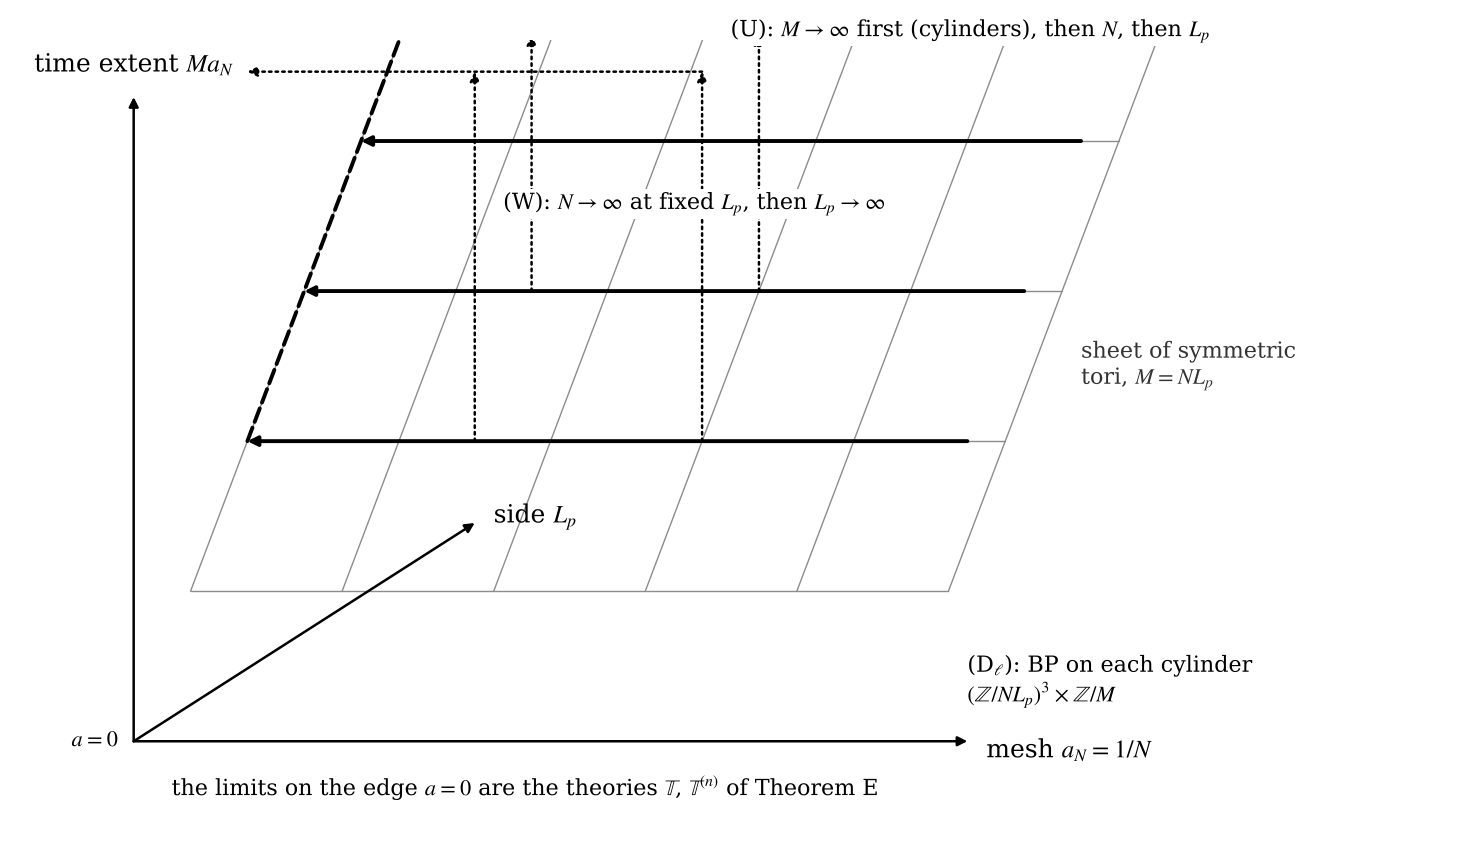
\includegraphics[width=\textwidth]{figures/fig_limits.png}
\caption{The two orders of the volume limits, in the space of mesh $a_N$, physical side $L_p$ and physical time extent $Ma_N$. The symmetric tori of (W) lie on the sheet where the time extent equals the side: the mesh is sent to zero at fixed $L_p$ along the sheet, then $L_p\to\infty$ along $a=0$ (solid and dashed arrows). The zero-temperature order sends the time extent to infinity first, on the cylinders where (D$_\ell$) is assumed, then the mesh, then the side (dotted arrows). Hypothesis (U), or its consequence of (Z) in Corollary~\ref{cor:Z}, is the statement that the two routes have the same end point.}
\label{fig:limits}
\end{figure}

\setcounter{mainthm}{4}
\begin{mainthm}[the bridge]\label{thm:E}
Let a continuum family satisfy \textup{(W)}, \textup{(U)} and
\textup{(D$_\ell$)}. Then $S^\chi$ does not depend on $\chi$, and the
Wightman theory of \textup{(W)} has Hamiltonian $H$ with
\[
\sigma(H)\subset\{0\}\cup[\Delta,\infty),\qquad\Delta=\frac{16\varpi}{625e^2\ell},
\]
with $0$ a simple eigenvalue.
\end{mainthm}
\setcounter{mainthm}{3}

The proof uses (W) only through the phase structure, the continuity in
$\chi$, the integrability of the phase correlations and the Wightman
property of the phases; the limit on symmetric tori enters through (U), or
through the weaker hypothesis (Z) of Section~\ref{ssec:thermalvacuum},
which implies the form of (U) that the proof needs. None of (W), (U), (Z)
or (D$_\ell$) is established in this paper for any four-dimensional family:
Theorem~\ref{thm:C} gives the cube condition at fixed strong coupling,
whereas (D$_\ell$) asks for it with $\varpi$ fixed and $n_N\le\ell N$ along
the couplings $\beta_{N,p}$ of a construction.

The proof occupies the rest of the section: the transfer matrix of a
cylinder (Sec.~\ref{ssec:transfermatrix}), its gap from the cube condition
(Sec.~\ref{ssec:cylindergap}), decay of the renormalised two-point functions
at zero temperature with a constant that survives the limit
(Sec.~\ref{ssec:zerotemp}), the Euclidean vectors of a Wightman theory
(Sec.~\ref{ssec:euclid}), and the assembly (Sec.~\ref{ssec:assembly}).

\subsection{The transfer matrix of a cylinder}\label{ssec:transfermatrix}

Fix $L$ and $\beta$. Let $\mathcal K=L^2(G^{E_0},\prod dQ_e)$ be the square
integrable functions of the spatial links of one time slice. For
configurations $Q,Q'$ of a slice and a family $U=(U_{\vec x})$ of temporal
link variables put
\[
S_s(Q)=\sum_{p\subset E_0}\ReTr Q_p,\qquad
S_0(Q,U,Q')=\sum_{\vec x,\,i}\ReTr\bigl(Q_{(\vec x,i)}U_{\vec x+e_i}
Q'^{\,*}_{(\vec x,i)}U^*_{\vec x}\bigr),
\]
the sums over the spatial plaquettes of the slice and over the timelike
plaquettes between two consecutive slices, and define the kernel
\begin{equation}\label{eq:transferkernel}
\mathbb T(Q,Q')=\int_{G^{(\Z/L\Z)^3}}\exp\Bigl(N\beta\bigl[\tfrac12S_s(Q)+\tfrac12S_s(Q')
+S_0(Q,U,Q')\bigr]\Bigr)\prod_{\vec x}dU_{\vec x}.
\end{equation}
For a function $F$ of the links of the slab $[0,w]$, $w\ge1$, let $\hat F$
be the operator on $\mathcal K$ with kernel
\begin{equation}\label{eq:slabkernel}
\begin{aligned}
\hat F(Q_0,Q_w)=\int&F(Q_0,U^{(0)},Q_1,\dots,U^{(w-1)},Q_w)\\
&\times\prod_{t=0}^{w-1}e^{N\beta[\frac12S_s(Q_t)+\frac12S_s(Q_{t+1})+S_0(Q_t,U^{(t)},Q_{t+1})]}
\prod_{t=1}^{w-1}dQ_t\prod_{t=0}^{w-1}dU^{(t)},
\end{aligned}
\end{equation}
and for $w=0$ let $\hat F$ be multiplication by $F$. Gauge transformations
$g=(g_{\vec x})$ of the slice act unitarily on $\mathcal K$ by $(R_gf)(Q)=
f(g\cdot Q)$.

\begin{lemma}[transfer matrix]\label{lem:transfer}
\begin{enumerate}[label=\textup{(\roman*)},leftmargin=*]
\item $\mathbb T$ is a self-adjoint Hilbert--Schmidt operator with a
continuous strictly positive kernel; its largest eigenvalue $\lambda_0>0$ is
simple, with a continuous eigenfunction $\Omega_0>0$, and every eigenfunction
with nonzero eigenvalue is gauge invariant. Every other eigenvalue has
modulus less than $\lambda_0$.
\item For $M\ge2$ the partition function of $\Lambda_{L,M}$ is $\Tr\mathbb T^M$.\footnote{The
spatial plaquettes of the slice $t$ carry weight $\frac12$ in each of the two
kernels $\mathbb T(Q_{t-1},Q_t)$ and $\mathbb T(Q_t,Q_{t+1})$, so they carry the
full Wilson weight exactly once around the cycle of $M$ slices, and the
temporal plaquettes between the slices $t$ and $t+1$ appear in $S_0(Q_t,
U^{(t)},Q_{t+1})$ only; the trace integrates over the $M$ slices and the
$M$ families of temporal links, which are all the links of $\Lambda_{L,M}$.}
\item Let $F$ be a bounded measurable function of the slab $[0,w]$ and $H$ one
of the slab $[0,w']$, and let $s\ge w$ and $M\ge s+w'$. Then
\[
\mu_{L,M}(F\,\tau_sH)=\frac{\Tr(\hat F\,\mathbb T^{s-w}\hat H\,\mathbb T^{M-s-w'})}
{\Tr\mathbb T^M}.
\]
\item The function $\vartheta\bar F$ is a function of the slab $[-w,0]$, and
for $s\ge0$ and $M\ge s+w+w'$
\[
\mu_{L,M}\bigl(\vartheta\bar F\,\tau_sH\bigr)=\frac{\Tr(\hat F^*\,\mathbb T^{s}
\hat H\,\mathbb T^{M-s-w-w'})}{\Tr\mathbb T^M}.
\]
\item For every bounded measurable function $F$ of a slab the limit
$\mu^0_{L}(F)=\lim_{M\to\infty}\mu_{L,M}(F)$ exists, and with $\Psi_F=
\lambda_0^{-w}\hat F\Omega_0$ and $\mathbb R=\mathbb T/\lambda_0$,
\[
\mu^0_L(\vartheta\bar F\,\tau_sH)=\ip{\Psi_F}{\mathbb R^s\Psi_H},\qquad
\mu^0_L(H)=\ip{\Omega_0}{\Psi_H}\qquad(s\ge0).
\]
\item If $F$ is gauge invariant then $R_g\hat F=\hat FR_g$ for every $g$.
\item If $\beta\ge0$ then $\mathbb T\ge0$ as an operator on $\mathcal K$.
\end{enumerate}
\end{lemma}

\begin{proof}
(i) The integrand of~\eqref{eq:transferkernel} is continuous and positive on
a compact space, so the kernel is continuous and strictly positive, and
$\mathbb T$ is Hilbert--Schmidt. Replacing $U_{\vec x}$ by $U_{\vec x}^{-1}$,
which preserves Haar measure, and using $\ReTr A=\ReTr A^*$ with the
cyclicity of the trace turns $S_0(Q,U,Q')$ into $S_0(Q',U,Q)$, so the kernel
is symmetric and $\mathbb T$ is self-adjoint. A simultaneous gauge
transformation $Q\mapsto g\cdot Q$, $Q'\mapsto g'\cdot Q'$ is absorbed by
$U_{\vec x}\mapsto g_{\vec x}^{-1}U_{\vec x}g'_{\vec x}$, so
$\mathbb T(g\cdot Q,g'\cdot Q')=\mathbb T(Q,Q')$; hence $\mathbb Tf$ is gauge
invariant for every $f$, and an eigenfunction with nonzero eigenvalue, being
in the range of $\mathbb T$, is gauge invariant and continuous. By Jentzsch's\footnote{Jentzsch's
theorem~\cite{Jen12}, in the form of~\cite[Ch.~V, \S6]{Sch74}: an integral
operator on $L^2(X,m)$, with $m$ a finite measure on a compact space $X$ and
a continuous kernel $k(x,y)>0$ everywhere, is compact, its spectral radius
$\lambda_0>0$ is an eigenvalue, simple, with an eigenfunction that is
strictly positive, and every other eigenvalue has modulus strictly less
than $\lambda_0$. Here $X=G^{E_0}$ with the product Haar measure, and the
kernel~\eqref{eq:transferkernel} is positive because the integrand is.}
theorem~\cite{Jen12}, in the form of~\cite[Thm.~V.6.6]{Sch74}, a compact
operator with a strictly positive kernel has its spectral radius as a simple
eigenvalue, with an almost everywhere positive eigenfunction, and every other
eigenvalue has smaller modulus; $\Omega_0=\lambda_0^{-1}\mathbb T\Omega_0$ is
continuous and strictly positive.

(ii) Write the Wilson weight of $\Lambda_{L,M}$ as the product over $t\in\Z/M\Z$
of $\exp(N\beta[\frac12S_s(Q_t)+\frac12S_s(Q_{t+1})+S_0(Q_t,U^{(t)},Q_{t+1})])$:
every spatial plaquette of slice $t$ appears with weight $\frac12$ in the
factors $t-1$ and $t$, and every timelike plaquette once. Integrating the
temporal links gives the kernel of $\mathbb T$ between consecutive slices, and
the integral over the slices is the trace of the $M$-fold product.

(iii) With the same factorisation, the slab $[0,w]$ contributes
$\hat F(Q_0,Q_w)$ after integrating its interior slices and temporal links,
the slab $[s,s+w']$ contributes $\hat H(Q_s,Q_{s+w'})$, and the remaining
$s-w$ and $M-s-w'$ factors contribute the powers of $\mathbb T$; when $s=w$
the shared slice $Q_w=Q_s$ is the integration variable of the composition
$\hat F\hat H$.

(iv) Under $\vartheta$ a temporal link from time $t$ to $t+1$ becomes the
link from $-t$ to $-t-1$, traversed backwards, which is the inversion in
(F3); the timelike plaquette weight is invariant, as in (i). So
$\vartheta\bar F$ is the function of the slab $[-w,0]$ whose kernel, in the
variables $(Q_{-w},Q_0)$, is $\overline{\hat F(Q_0,Q_{-w})}=\hat F^*(Q_{-w},Q_0)$.
Now apply (iii) to the slabs $[-w,0]$ and $[s,s+w']$.

(v) Let $P_0$ be the projection on $\Omega_0$ and $\mathbb R=\mathbb T/\lambda_0=
P_0+\mathbb S$ with $\|\mathbb S\|<1$ by (i). Since $\mathbb T^2$ is trace
class, $\|\mathbb S^{k}\|_1\le\|\mathbb S^2\|_1\|\mathbb S\|^{k-2}\to0$, so
$\Tr(A\mathbb R^{M-c})/\Tr\mathbb R^M\to\ip{\Omega_0}{A\Omega_0}$ for every
bounded $A$ and fixed $c$. Apply this to (iii) with $H=1$ for the existence of
the limit and to (iv) for the formula: $\Tr(\hat F^*\mathbb T^s\hat H
\mathbb T^{M-s-w-w'})/\Tr\mathbb T^M\to\lambda_0^{-s-w-w'}\ip{\Omega_0}
{\hat F^*\mathbb T^s\hat H\Omega_0}$.

(vi) The kernel~\eqref{eq:slabkernel} is invariant under simultaneous gauge
transformations of all slices of the slab, by the invariance of $F$ and the
substitution of (i) for the temporal links, so $\hat F(g\cdot Q_0,g\cdot Q_w)=
\hat F(Q_0,Q_w)$.

(vii) Put $f(g)=e^{N\beta\ReTr g}$ on $G$ and $c=N\beta\ge0$. Since $\ReTr g=
\frac12(\chi(g)+\overline{\chi(g)})$ with $\chi=\Tr$ the character of the
defining representation,
\[
f=\sum_{a,b\ge0}\frac{(c/2)^{a+b}}{a!\,b!}\,\chi^a\bar\chi^{\,b},
\]
uniformly on $G$, and $\chi^a\bar\chi^{\,b}$ is the character of
$(\C^N)^{\otimes a}\otimes(\overline{\C^N})^{\otimes b}$, a sum of irreducible
characters with nonnegative integer coefficients. Hence $f=\sum_\lambda
f_\lambda\chi_\lambda$ with $f_\lambda\ge0$, and as $\chi_\lambda(x^{-1}y)=
\sum_{a,b}\overline{D^\lambda_{ab}(x)}D^\lambda_{ab}(y)$ in a unitary basis,
$f(x^{-1}y)$ is a positive definite kernel on $G$; so is $f(xy^{-1})=
f(y^{-1}x)=f(x^{-1}y)$, by conjugation invariance and $\ReTr g=\ReTr g^{-1}$. By Schur's product theorem\footnote{The
entrywise product of two positive semidefinite matrices $(a_{ij})$,
$(b_{ij})$ is positive semidefinite, because it is the principal submatrix
of the tensor product $(a_{ij}b_{kl})$ on the diagonal pairs $(i,i)$, and the
tensor product of positive semidefinite matrices is positive semidefinite.
Applied to finite sections of continuous kernels this shows that the
product of positive definite kernels is positive definite.} the
kernel $K(Q,Q')=\prod_{e\in E_0}f(Q_eQ_e'^{\,*})$ is positive definite on
$G^{E_0}$, and being continuous it defines a nonnegative Hilbert--Schmidt
operator $K$ on $\mathcal K$. The substitution $Q'\mapsto U\cdot Q'$,
$(U\cdot Q')_{(\vec x,i)}=U_{\vec x}Q'_{(\vec x,i)}U^*_{\vec x+e_i}$, turns
$S_0(Q,U,Q')$ into $\sum\ReTr(Q_{(\vec x,i)}(U\cdot Q')^*_{(\vec x,i)})$, so
\[
\mathbb T=D\Bigl(\int K\circ R_{U}^{\,-1}\ \prod_{\vec x}dU_{\vec x}\Bigr)D
=D\,K\,\Pi\,D=D\,\Pi K\Pi\,D,
\]
where $D$ is multiplication by $e^{N\beta S_s/2}$, $\Pi=\int R_U\,dU$ is the
orthogonal projection on the gauge-invariant functions, and $K$ commutes with
every $R_g$ because $K(g\cdot Q,g\cdot Q')=K(Q,Q')$. Thus $\mathbb T=
(K^{1/2}\Pi D)^*(K^{1/2}\Pi D)\ge0$.
\end{proof}

The state $\mu^0_L$ is the zero-temperature state of the cylinder of
spatial side $L$: by (v) it is the expectation in the vector $\Omega_0$ of
the time-ordered products of slab operators, and $\mu_{L,M}$ is the
corresponding thermal state at temperature $1/M$.

\begin{figure}[t]
\centering
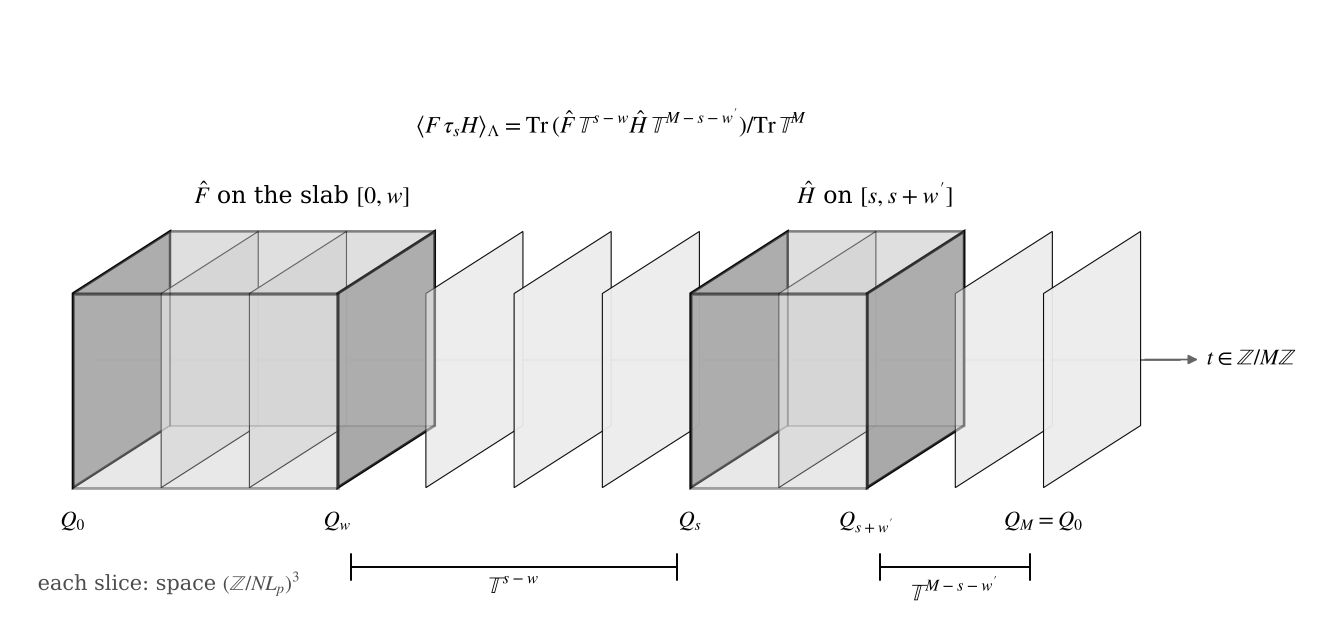
\includegraphics[width=\textwidth]{figures/fig_transfer.png}
\caption{The cylinder $\Lambda_{L,M}$ sliced in time. A function $F$ of the slab $[0,w]$ becomes the integral operator $\hat F$ on the slice space $\mathcal K$, a function $H$ of the slab $[s,s+w']$ becomes $\hat H$, and the time steps between the slabs are powers of the transfer matrix $\mathbb T$; the trace formula is Lemma~\ref{lem:transfer}(iii), and the reflected form, with $\hat F^*$, is Lemma~\ref{lem:transfer}(iv).}
\label{fig:transfer}
\end{figure}

\subsection{The gap of the transfer matrix from the cube condition}
\label{ssec:cylindergap}

\begin{proposition}[cylinder gap]\label{prop:cylindergap}
Let $n\ge2$, $\varpi>0$, $L\ge2n+4$, and suppose $\BP(n,\varpi)$ holds for
$\mu_{L,M}$ for every $M\ge2n+4$. Then every eigenvalue $\lambda\ne\lambda_0$ of
$\mathbb T$ satisfies
\[
\frac{|\lambda|}{\lambda_0}\le e^{-m_n},\qquad m_n=\frac{\varpi}{e^2q_nn}.
\]
\end{proposition}

\begin{proof}
Let $F$ be a real continuous gauge-invariant function of the slice $E_0$
with $|F|\le1$, depending on a set $S$ of links, and let $s\ge3n-2$ be
even. On $\Lambda_{L,M}$ with $M\ge2s$ the functions $F$ and $\tau_sF$ depend
on links whose base points differ by $s$ in time, so $d(S,\tau_sS)=s$; as
$s\ge3n-2$ and $n\ge2$, $M\ge2s\ge6n-4\ge2n+4$, so all sides of
$\Lambda_{L,M}$ are at least $2n+4$, $\BP(n,\varpi)$ holds for $\mu_{L,M}$,
and Theorem~\ref{thm:decay} gives
\[
\bigl|\mu_{L,M}(F\,\tau_sF)-\mu_{L,M}(F)^2\bigr|\le
\Bigl(e+\frac{k|S|^2}{64e^2}\Bigr)e^{-\varpi k/(e^2q_n)},\qquad
k=\Bigl\lfloor\frac{s+2}n\Bigr\rfloor-2 ,
\]
uniformly in $M$. Let $M\to\infty$: by Lemma~\ref{lem:transfer}(v) with
$w=w'=0$ and $\vartheta\bar F=F$, the left side becomes
$\ip{F\Omega_0}{\mathbb R^sF\Omega_0}-\ip{\Omega_0}{F\Omega_0}^2=
\sum_{j\ge1}r_j^s|\ip{\phi_j}{F\Omega_0}|^2$, where $(\phi_j)_{j\ge0}$ is an
orthonormal eigenbasis of $\mathbb T$ with real eigenvalues $\lambda_j=r_j
\lambda_0$, $\phi_0=\Omega_0$. As $s$ is even every term is nonnegative, and
$s/n-3<k\le s/n$, so for each $j\ge1$
\[
|r_j|^s\,|\ip{\phi_j}{F\Omega_0}|^2\le\Bigl(e+\frac{(s/n)|S|^2}{64e^2}\Bigr)
e^{3\varpi/(e^2q_n)}e^{-m_ns}.
\]
Letting $s\to\infty$ through even values gives $|r_j|\le e^{-m_n}$ whenever
$\ip{\phi_j}{F\Omega_0}\ne0$ for some such $F$. It remains to see that the
vectors $F\Omega_0$, $F$ real, span a dense subspace of the gauge-invariant
part of $\mathcal K$, which contains every $\phi_j$ with $\lambda_j\ne0$ by
Lemma~\ref{lem:transfer}(i). Let $h$ be gauge invariant and square
integrable. Since $\Omega_0$ is continuous, strictly positive and gauge
invariant, $h/\Omega_0$ is gauge invariant and square integrable for the
finite measure $\Omega_0^2\prod dQ_e$, and the continuous gauge-invariant
functions are dense in that space, because averaging a continuous
approximant over the compact gauge group preserves the approximation. If
$F_k\to h/\Omega_0$ there, then $\|F_k\Omega_0-h\|_{\mathcal K}\to0$; the real
and imaginary parts of $F_k$ are real continuous gauge-invariant functions.
\end{proof}

The proposition needs the cube condition on cylinders of every time period
and fixed spatial side: on a single symmetric torus the two-point function
of a bounded observable at separation $s\le M/2$ contains the thermal terms
$r_i^{M-s}r_j^{s}$, and a bound of the form $Ce^{-ms}$ for $s\le M/2$ at one
value of $M$ only gives $r_1\le e^{-m}(Cz)^{2/M}$ with $z=\Tr\mathbb R^M$, which tends to $e^{-m}$
as $M\to\infty$ at fixed coupling but not along a tuning in which the
coupling changes with $M$.

\subsection{Decay of renormalised two-point functions at zero temperature}
\label{ssec:zerotemp}

\begin{lemma}[gap to decay, with a surviving constant]\label{lem:gaptodecay}
Suppose every eigenvalue $\lambda\ne\lambda_0$ of $\mathbb T$ satisfies $|\lambda|
\le e^{-m}\lambda_0$. Let $F$ and $H$ be bounded measurable functions of the
slabs $[0,w]$ and $[0,w']$, let $\Psi'_F=\Psi_F-\ip{\Omega_0}{\Psi_F}\Omega_0$,
and put $C_F(s)=\mu^0_L(\vartheta\bar F\,\tau_sF)-|\mu^0_L(F)|^2=
\ip{\Psi'_F}{\mathbb R^s\Psi'_F}\ge0$. Then for all integers $s\ge s_1\ge0$,
\[
\bigl|\mu^0_L(\vartheta\bar F\,\tau_sH)-\overline{\mu^0_L(F)}\,\mu^0_L(H)\bigr|
\le e^{-m(s-s_1)}\sqrt{C_F(s_1)\,C_H(s_1)} .
\]
\end{lemma}

\begin{proof}
By Lemma~\ref{lem:transfer}(v) the left side is $|\ip{\Psi'_F}{\mathbb R^s
\Psi'_H}|$, since $\mathbb R\Omega_0=\Omega_0$ and $\Psi'_F\perp\Omega_0$. By
Lemma~\ref{lem:transfer}(vii), $\mathbb R\ge0$, so $\mathbb R^{s_1/2}$ is
defined by the functional calculus, and $\mathbb R^{s}=\mathbb R^{s_1/2}\,
\mathbb R^{s-s_1}\,\mathbb R^{s_1/2}$. The subspace $\Omega_0^\perp$ is
invariant under $\mathbb R$, on which $\|\mathbb R\|\le e^{-m}$, so the
Cauchy--Schwarz inequality gives $|\ip{\Psi'_F}{\mathbb R^s\Psi'_H}|\le
e^{-m(s-s_1)}\|\mathbb R^{s_1/2}\Psi'_F\|\,\|\mathbb R^{s_1/2}\Psi'_H\|$, and
$\|\mathbb R^{s_1/2}\Psi'_F\|^2=\ip{\Psi'_F}{\mathbb R^{s_1}\Psi'_F}=C_F(s_1)$.
\end{proof}

The point of the lemma is the constant. For a renormalised cluster the
norms $\|\Psi_F\|$, the suprema $\|F\|_\infty$ and the variances of $F$ under
the lattice measure diverge as $N\to\infty$, so the covariance bound of
Theorem~\ref{thm:decay} is useless for such $F$; the quantity $C_F(s_1)$ is
the connected two-point function of the cluster with its reflection at the
positive separation $s_1$, which under (U) converges to a Schwinger function
at separated points.

\subsection{Euclidean vectors of a Wightman theory}\label{ssec:euclid}

Let $(\mathcal H,\Omega,U)$ carry a Wightman theory in the sense
of~\cite[Ch.~3]{SW64}: a unitary representation $U(a,\Lambda)$ of the
Poincar\'e group with energy--momentum $P$ satisfying the spectrum condition
$\sigma(P)\subset\overline{V_+}$, a unique invariant unit vector $\Omega$,
and operator-valued tempered distributions $\Phi_v$, $v\in V$, on a common
dense invariant domain containing $\Omega$, covariant under $U$ and local,
with $\Omega$ cyclic for the polynomials in the fields, and with
$\Phi_{v^\vartheta}(f)=\Phi_v(\bar f)^*$ on the domain. Let $H=P^0\ge0$. We use
the metric $p\cdot z=p^0z^0-\vec p\cdot\vec z$ and $U(a)=e^{iP\cdot a}$, and the
forward tube
\[
\mathfrak T_m=\bigl\{z\in(\C^4)^m:\ \operatorname{Im}z_1\in V_+,\
\operatorname{Im}(z_{j+1}-z_j)\in V_+\ (1\le j<m)\bigr\}.
\]
A Euclidean point $x=(x_1,\dots,x_m)\in(\R^4)^m$ with times $0<\tau_1<\dots<
\tau_m$ corresponds to $\hat x=((i\tau_1,\vec x_1),\dots,(i\tau_m,\vec x_m))
\in\mathfrak T_m$.

\begin{lemma}[Euclidean vectors]\label{lem:wightman}
\begin{enumerate}[label=\textup{(\roman*)},leftmargin=*]
\item For $\mathbf v\in V^m$ there is a holomorphic function $\Psi_{\mathbf v}:
\mathfrak T_m\to\mathcal H$ whose boundary value as $\operatorname{Im}z\to0$
inside the tube is the vector-valued distribution $\Phi_{v_1}(x_1)\cdots
\Phi_{v_m}(x_m)\Omega$.
\item For a cluster $(\mathbf v,t)$ with $t$ supported in the configurations
with $0<\tau_1<\dots<\tau_m$, the vector $\psi(\mathbf v,t)=\int t(x)
\Psi_{\mathbf v}(\hat x)\,dx$ satisfies $\ip\Omega{\psi(\mathbf v,t)}=
\int t\,S_{\mathbf v}$ and, for $\sigma\ge0$ and a second such cluster,
\[
\ip{\psi(\mathbf v,t)}{e^{-\sigma H}\psi(\mathbf v',t')}=\int(\Theta\bar t\otimes
\tau_\sigma t')\,S_{\mathbf v^\vartheta\mathbf v'},\qquad
\mathbf v^\vartheta=(v_1^\vartheta,\dots,v_m^\vartheta),
\]
where $S_{\mathbf u}$ are the Schwinger functions, defined as follows. The
vacuum expectation $W_{\mathbf u}(x)=\ip\Omega{\Phi_{u_1}(x_1)\cdots
\Phi_{u_k}(x_k)\Omega}$ is the boundary value of a function
$W_{\mathbf u}(\zeta)$ holomorphic in the difference tube
\[
\mathfrak T'_k=\bigl\{\zeta\in(\C^4)^k:\ \operatorname{Im}(\zeta_{j+1}-\zeta_j)
\in V_+\ (1\le j<k)\bigr\},
\]
and $S_{\mathbf u}(x)=W_{\mathbf u}(\hat x)$ when $\tau_1<\dots<\tau_k$,
extended to the configurations with distinct times by permutation
symmetry.
\item The vectors $\psi(\mathbf v,t)$ of (ii), over all $m\ge1$, $\mathbf v$
and $t$, together with $\Omega$, span a dense subspace of $\mathcal H$.
\end{enumerate}
\end{lemma}

\begin{proof}
(i) The map $(f_1,\dots,f_m)\mapsto\Phi_{v_1}(f_1)\cdots\Phi_{v_m}(f_m)\Omega$
is multilinear and separately continuous from $\mathcal S(\R^4)^m$ to
$\mathcal H$, hence jointly continuous, and extends to a continuous linear map
$f\mapsto\Psi_{\mathbf v}(f)$ on $\mathcal S(\R^{4m})$ by the nuclear
theorem. Write $x_j=x_1+\xi_1+\dots+\xi_{j-1}$. Since $\Phi_{v_j}(x_j)\cdots
\Phi_{v_m}(x_m)\Omega=U(x_j)\Phi_{v_j}(0)\Phi_{v_{j+1}}(x_{j+1}-x_j)\cdots\Omega$
in the sense of distributions, the Fourier transform of $\Psi_{\mathbf v}$ in
the variable $x_1$ is supported in $\overline{V_+}$, and so is its Fourier
transform in each $\xi_j$, by the spectrum condition applied to the vector
to the right of $U(\xi_j)$. For every $\chi\in\mathcal H$ the scalar
distribution $\ip\chi{\Psi_{\mathbf v}(\cdot)}$ therefore has Fourier
transform supported in the closed convex cone $\overline{V_+}^{\,m}$ in these
variables, so it is the boundary value of a function holomorphic in
$\mathfrak T_m$~\cite[Thm.~2-8]{SW64}; the family of these distributions over
$\|\chi\|\le1$ is bounded in $\mathcal S'$, so the holomorphic functions are
uniformly bounded on compact subsets of the tube, and they define a weakly,
hence strongly, holomorphic $\Psi_{\mathbf v}:\mathfrak T_m\to\mathcal H$ with
$\ip\chi{\Psi_{\mathbf v}(z)}$ equal to these continuations.

(ii) The vacuum expectation $W_{\mathbf u}$ is translation invariant, and the
argument of (i) applied to the differences shows that it is the boundary
value of a function holomorphic in $\mathfrak T'_k$; for $x$ with increasing
times, $\hat x\in\mathfrak T'_k$ and $W_{\mathbf u}(\hat x)=\ip\Omega{\Psi_{\mathbf u}
(\hat x)}$ when the times are positive, by (i) and translation invariance, so
the first identity holds. For the second, let $z\in\mathfrak T_m$ and $z'\in
\mathfrak T_{m'}$. The function $(z,z')\mapsto\ip{\Psi_{\mathbf v}(z)}{
\Psi_{\mathbf v'}(z')}$ is antiholomorphic in $z$ and holomorphic in $z'$, and
by $\Phi_{v^\vartheta}(f)=\Phi_v(\bar f)^*$ its boundary value is the
distribution $W_{\check{\mathbf v}^\vartheta\mathbf v'}(x_m,\dots,x_1,y_1,\dots,
y_{m'})$, $\check{\mathbf v}^\vartheta=(v_m^\vartheta,\dots,v_1^\vartheta)$. The
map $(z,z')\mapsto(\bar z_m,\dots,\bar z_1,z'_1,\dots,z'_{m'})$ sends
$\mathfrak T_m\times\mathfrak T_{m'}$ into $\mathfrak T'_{m+m'}$: the
imaginary parts of the consecutive differences are $\operatorname{Im}(z_{j+1}
-z_j)$, $\operatorname{Im}z_1+\operatorname{Im}z'_1$ and $\operatorname{Im}
(z'_{j+1}-z'_j)$, all in $V_+$. Two functions holomorphic in $(\bar z,z')$ on
this product of tubes with the same distributional boundary
value coincide~\cite[Ch.~2]{SW64}, so
\[
\ip{\Psi_{\mathbf v}(z)}{\Psi_{\mathbf v'}(z')}=W_{\check{\mathbf v}^\vartheta\mathbf v'}
(\bar z_m,\dots,\bar z_1,z'_1,\dots,z'_{m'}).
\]
Next, $U(a)\Psi_{\mathbf v'}(z')=\Psi_{\mathbf v'}(z'+a)$ for real $a$ by
covariance; both sides are holomorphic in $a$ on the tube
$\operatorname{Im}a\in V_+$ with these boundary values, the left by the
spectrum condition and the right because $z'+a\in\mathfrak T_{m'}$, so they
agree there, and $e^{-\sigma H}\Psi_{\mathbf v'}(\hat y)=\Psi_{\mathbf v'}
(\widehat{\tau_\sigma y})$. At the Euclidean points $z=\hat x$, $z'=
\widehat{\tau_\sigma y}$ one has $\bar z_j=\widehat{\vartheta x_j}$, and the
times $-\tau_m<\dots<-\tau_1<\sigma+\tau'_1<\dots$ increase, so
\[
\ip{\Psi_{\mathbf v}(\hat x)}{e^{-\sigma H}\Psi_{\mathbf v'}(\hat y)}
=S_{\check{\mathbf v}^\vartheta\mathbf v'}(\vartheta x_m,\dots,\vartheta x_1,
\tau_\sigma y_1,\dots,\tau_\sigma y_{m'}).
\]
Integrate against $\bar t(x)t'(y)$ and substitute $u_i=\vartheta x_{m+1-i}$;
the permutation symmetry
\[
S_{\check{\mathbf v}^\vartheta\mathbf v'}(u_m,\dots,u_1,y)=S_{\mathbf v^\vartheta
\mathbf v'}(u_1,\dots,u_m,y)
\]
turns the result into $\int\overline{t(\vartheta u_1,\dots,\vartheta u_m)}\,
(\tau_\sigma t')(y)\,S_{\mathbf v^\vartheta\mathbf v'}(u,y)\,du\,dy$, which is
the claim.

(iii) Let $\chi\perp\Omega$ and $\chi\perp\psi(\mathbf v,t)$ for all clusters
of (ii). Then the
holomorphic function $\ip\chi{\Psi_{\mathbf v}(z)}$ vanishes on the open
subset $\{\hat x\}$ of the totally real submanifold $\{(i\tau_j,\vec x_j)\}
\cap\mathfrak T_m$, which has real dimension $4m$; after the complex-linear
change of coordinates $z^0_j\mapsto-iz^0_j$ this is an open subset of
$\R^{4m}$, so the function vanishes on the connected tube. Its boundary
value $\ip\chi{\Phi_{v_1}(x_1)\cdots\Phi_{v_m}(x_m)\Omega}$ then vanishes as a
distribution, for all $m$ and $\mathbf v$, so $\chi$ is orthogonal to the
polynomials in the fields applied to $\Omega$, which are dense, and to
$\Omega$ itself.
\end{proof}

\subsection{Proof of Theorem~\ref{thm:E}}\label{ssec:assembly}

\emph{Step 1: the lattice inequality.} Fix $N$ and $p$ large, put $L=NL_p$,
$n=n_N$ and $a=a_N$, and let $\mathbb T$ be the transfer matrix of the
cylinder of side $L$ at coupling $\beta_{N,p}$. Since $n_N\le\ell N$, one has
$L\ge2n_N+4$ as soon as $L_p\ge2\ell+1$ and $N\ge4$, which holds for $p$ and
$N$ large; so by (D$_\ell$) and Proposition~\ref{prop:cylindergap},
$\mathbb T$ has gap $m_n=\varpi/(e^2q_nn)$. Let $(\mathbf v,t)$ and
$(\mathbf v',t')$ be clusters with $t,t'$ supported in configurations whose
times lie in $(\delta,\omega)$, $0<\delta<\omega$, and let $\rho\ge0$ be such
that $R_v\subset\Z^3\times[-\rho,\rho]$ for the finitely many tokens $v$ of
$\mathbf v,\mathbf v'$, a link being in $x+R_v$ when its base point is. For
$N>\rho/\delta$ a site $x$ with $t(ax)\ne0$ has time $x^0\in(\delta N,\omega
N)$, so the links of $x+R_v$ have end points at times in $[x^0-\rho,x^0+\rho
+1]\subset[0,\lceil\omega N\rceil+\rho]$; hence the lattice functions
\[
F=a^{4m}\sum_xt(ax)\prod_i\Phi^{N,p}_{v_i}(x_i,\cdot),\qquad
H=a^{4m'}\sum_yt'(ay)\prod_j\Phi^{N,p}_{v'_j}(y_j,\cdot)
\]
are bounded, gauge invariant, and depend on the links of the slab
$[0,w]$ with $w=\lceil\omega N\rceil+\rho$. Let $\sigma\ge\sigma_1\ge1$ be integers.
Lemma~\ref{lem:gaptodecay} with $s=\sigma N$, $s_1=\sigma_1N$ gives
\begin{equation}\label{eq:latticeineq}
\bigl|\mu^0_L(\vartheta\bar F\,\tau_{\sigma N}H)-\overline{\mu^0_L(F)}\mu^0_L(H)\bigr|
\le e^{-m_nN(\sigma-\sigma_1)}\sqrt{C_F(\sigma_1N)C_H(\sigma_1N)},
\end{equation}
and $m_nN=\varpi/(e^2q_nna)\ge\Delta$ because $na\le\ell$ and $q_n\le625/16$.
Each quantity in~\eqref{eq:latticeineq} is a zero-temperature smear $S^0_{N,p}$
of a cluster: by (F3), $\vartheta\bar F=a^{4m}\sum_y(\Theta\bar t)(ay)\prod_i
\Phi^{N,p}_{v_i^\vartheta}(y_i,\cdot)$, and by (F2), $\tau_{\sigma N}H=a^{4m'}
\sum_y(\tau_\sigma t')(ay)\prod_j\Phi^{N,p}_{v'_j}(y_j,\cdot)$ since $\sigma N
\in\Z$; so $\mu^0_L(\vartheta\bar F\,\tau_{\sigma N}H)$ is the smear of
$c_1=(\mathbf v^\vartheta\mathbf v',\Theta\bar t\otimes\tau_\sigma t')$,
$\mu^0_L(F)$ and $\mu^0_L(H)$ those of $c_2=(\mathbf v,t)$ and $c_3=(\mathbf v',
t')$, and $C_F(\sigma_1N)$ is the smear of $c_4=(\mathbf v^\vartheta\mathbf v,
\Theta\bar t\otimes\tau_{\sigma_1}t)$ minus $|S^0_{N,p}(\mathbf v,t)|^2$. The product clusters are supported in
$D_{m+m'}$ because reflected and translated times are separated by at least
$2\delta$.

\emph{Step 2: the limit.} Let $N\to\infty$ along the progression and then
$p\to\infty$ along the sequence of (W). By (U) every smear
in~\eqref{eq:latticeineq} converges to the $\nu$-average of the corresponding
phase correlation. Writing $\bar S(\cdot)=\int_XS^\chi(\cdot)\,d\nu$ and
$\bar S^c(t,t';\sigma)=\bar S(\mathbf v^\vartheta\mathbf v',\Theta\bar t
\otimes\tau_\sigma t')-\overline{\bar S(\mathbf v,t)}\,\bar S(\mathbf v',t')$,
\begin{equation}\label{eq:limitineq}
|\bar S^c(t,t';\sigma)|\le e^{-\Delta(\sigma-\sigma_1)}\sqrt{\bar S^c(t,t;\sigma_1)
\,\bar S^c(t',t';\sigma_1)}
\end{equation}
for all integers $1\le\sigma_1\le\sigma$, the right side being nonnegative as a
limit of nonnegative numbers.

\emph{Step 3: the phases coincide.} For $\nu$-almost every $\chi$ the phase is
a Wightman theory, and by Lemma~\ref{lem:wightman}(ii) its own connected
function $S^{\chi,c}(t,t;\sigma)=\|e^{-\sigma H_\chi/2}\psi_\chi'\|^2\ge0$, with
$\psi'_\chi=\psi_\chi(\mathbf v,t)-\ip{\Omega_\chi}{\psi_\chi(\mathbf v,t)}
\Omega_\chi$. Hence
\[
\bar S^c(t,t;\sigma)=\int_XS^{\chi,c}(t,t;\sigma)\,d\nu(\chi)+\operatorname{Var}_\nu
\bigl(S^\chi(\mathbf v,t)\bigr)\ge\operatorname{Var}_\nu\bigl(S^\chi(\mathbf v,t)\bigr),
\]
the variance being finite because $|S^\chi(\mathbf v,t)|^2\le\|\psi_\chi
(\mathbf v,t)\|^2=S^\chi(\mathbf v^\vartheta\mathbf v,\Theta\bar t\otimes t)$ is
$\nu$-integrable by (W); while by~\eqref{eq:limitineq} with $t'=t$ the left
side tends to $0$ as $\sigma\to\infty$. So $S^\chi(\mathbf v,t)=\bar S(\mathbf v,t)$
for $\nu$-almost every $\chi$, for every cluster whose times are ordered in
some $(\delta,\omega)$. Fix $m$, $\mathbf v\in V^m$ and the open set
$\mathcal O=\{0<\tau_1<\dots<\tau_m\}\subset D_m$, and a countable set
$\mathcal D\subset C^\infty_c(\mathcal O)$ such that every $t\in C^\infty_c
(\mathcal O)$ is a uniform limit of elements of $\mathcal D$ supported in a
fixed compact subset of $\mathcal O$. As $V$ is countable, there is a
$\nu$-null set $X_1$ such that for $\chi\notin X_1$ the phase is a Wightman
theory and $S^\chi(\mathbf v,t)=\bar S(\mathbf v,t)$ for all $m$, $\mathbf v$
and $t\in\mathcal D$. For $\chi,\chi'\notin X_1$ the continuous function
$S^\chi_{\mathbf v}-S^{\chi'}_{\mathbf v}$ integrates to $0$ against every
$t\in\mathcal D$, hence against every $t\in C^\infty_c(\mathcal O)$, hence
vanishes on $\mathcal O$; by translation invariance in time and the
permutation symmetry of the Schwinger functions it vanishes at every
configuration with distinct times, and by continuity on $D_m$. Fix $\chi_0
\notin X_1$. For $x\in D_m$ the set $\{\chi:S^\chi_{\mathbf v}(x)=
S^{\chi_0}_{\mathbf v}(x)\}$ is closed by (W) and contains $X\setminus X_1$,
which is dense because $\nu$ has full support and $\nu(X_1)=0$; so it is
$X$. Thus $S^\chi=S^{\chi_0}$ for every $\chi$, $\bar S=S^{\chi_0}$, and
\eqref{eq:limitineq} holds for the Schwinger functions of the Wightman theory
of (W), call it $(\mathcal H,\Omega,H)$.

\emph{Step 4: the spectrum.} By Lemma~\ref{lem:wightman}(ii),
\eqref{eq:limitineq} with $t'=t$ reads, for the vector $\psi'=\psi(\mathbf v,t)
-\ip\Omega{\psi(\mathbf v,t)}\Omega\perp\Omega$,
\[
\ip{\psi'}{e^{-\sigma H}\psi'}\le e^{-\Delta(\sigma-\sigma_1)}\ip{\psi'}{e^{-\sigma_1H}\psi'}
\qquad(\sigma\ge\sigma_1\ge1\text{ integers}).
\]
If $\kappa$ is the spectral measure of $H$ at $\psi'$ and $0<\eta<\Delta$,
then $e^{-\sigma(\Delta-\eta)}\kappa([0,\Delta-\eta])\le e^{-\Delta(\sigma-\sigma_1)}
\kappa([0,\infty))$, so $\kappa([0,\Delta-\eta])\le e^{\Delta\sigma_1}\|\psi'\|^2
e^{-\eta\sigma}\to0$. Hence the spectral projection $E_H([0,\Delta-\eta])$
annihilates $\psi'$, that is $E_H([0,\Delta-\eta])\psi(\mathbf v,t)=
\ip\Omega{\psi(\mathbf v,t)}\Omega$, for every cluster with ordered times in
some interval $(\delta,\omega)$; every cluster of Lemma~\ref{lem:wightman}(ii)
is of this form. These vectors and $\Omega$, for which the identity is
trivial, span a dense subspace by Lemma~\ref{lem:wightman}(iii), so
$E_H([0,\Delta-\eta])$ is the projection on $\C\Omega$ for every $\eta>0$:
the spectrum of $H$ lies in $\{0\}\cup[\Delta,\infty)$ and $0$ is simple.
\qed

\begin{remark}[why the symmetric order needs \textup{(U)}]\label{rem:thermal}
On the symmetric torus the thermal two-point function of a slab function is
\[
\mu_{L,L}(\vartheta\bar F\,\tau_sF)=\frac{\lambda_0^{-2w}}{\Tr\mathbb R^L}
\sum_{i,j}r_i^{L-s-2w}r_j^{s}|\ip{\phi_j}{\hat F\phi_i}|^2,
\]
a sum of exponentials $e^{-s(E_j-E_i)}$ in which both signs of $E_j-E_i$
occur. It is convex, symmetric about $s=L/2-w$ when $\hat F$ is self-adjoint,
and it is not the Laplace transform of a positive measure on $[0,\infty)$
unless the terms with $i\ge1$ vanish. Those terms are bounded, by the log-convexity of
$\theta\mapsto\Tr(\mathbb T^{\theta}A\mathbb T^{1-\theta}A^*)$, by the
two-point functions at adjacent separation, but no bound on their sum that
is uniform in $N$ follows from the gap of $\mathbb T$ alone: it would require
a bound on $\sum_{i\ge1}r_i^{L}$, the thermal partition function of the
torus relative to its vacuum, uniformly in the lattice spacing, which is a
statement about the density of states up to the cutoff. Hypothesis (U)
replaces that estimate by the statement that the two orders of the volume
limits agree, and nothing in Theorem~\ref{thm:E} uses more. The next
subsection shows that the estimate is also sufficient: a bound on
$\sum_{i\ge1}r_i^L$ alone, hypothesis (Z) below, implies the form of (U)
that the proof uses.
\end{remark}

\begin{figure}[t]
\centering
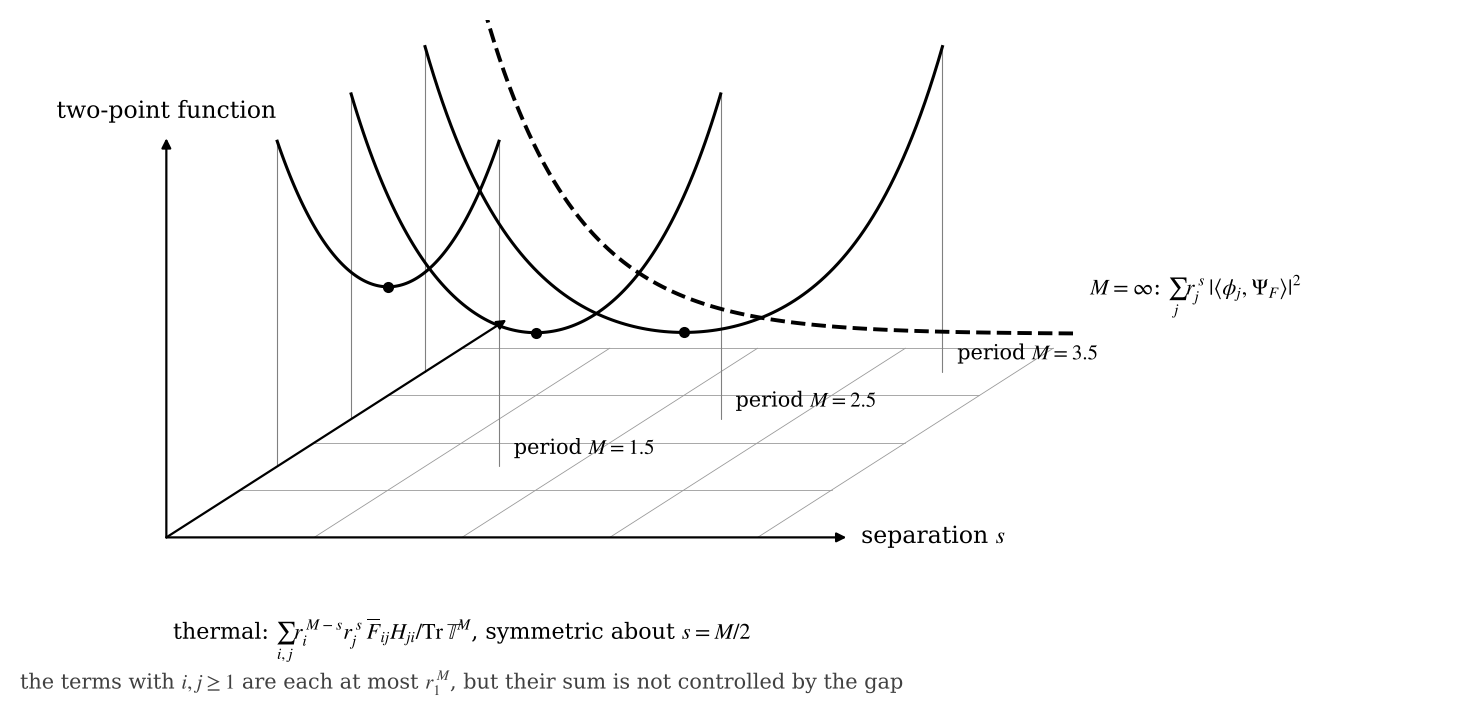
\includegraphics[width=\textwidth]{figures/fig_thermal.png}
\caption{Two-point functions of one slab observable on cylinders of physical period $M$ and at zero temperature ($M=\infty$), for one excited level of $\mathbb R$: the thermal function contains the terms $r_i^{M-s}r_j^{s}$ with both signs of $E_j-E_i$ and is symmetric about $s=M/2$ (Remark~\ref{rem:thermal}), while the zero-temperature function is the Laplace transform of a positive measure, which is what Lemma~\ref{lem:gaptodecay} uses. The terms with $i,j\ge1$ are each at most $r_1^{\,M}$, but their number is not controlled by the gap; Lemma~\ref{lem:thermaldiscrepancy} bounds their total by $\mathcal Z_L(M)-1$.}
\label{fig:thermal}
\end{figure}

\subsection{Thermal states against the vacuum}\label{ssec:thermalvacuum}

Fix $L$ and $\beta$, let $\mathbb T$, $\lambda_0$, $\Omega_0$ and $\mathbb R=
\mathbb T/\lambda_0$ be as in Lemma~\ref{lem:transfer}, and for $M\ge2$ put
\[
\mathcal Z_L(M)=\Tr\mathbb R^M=\frac{Z(\Lambda_{L,M})}{\lambda_0^M}\ \ge1,
\]
the partition function of $\Lambda_{L,M}$ relative to the vacuum of the
cylinder. By Lemma~\ref{lem:transfer}(i),(ii), $\lambda_0=\lim_{M\to\infty}
Z(\Lambda_{L,M})^{1/M}$, so $\mathcal Z_L(M)$ is determined by the Wilson
partition functions alone and involves no insertion.\footnote{In the
language of statistical mechanics, $-\log\lambda_0$ is the ground-state
energy of the cylinder Hamiltonian $H_L=-\log\mathbb T$ restricted to the
range of $\mathbb T$, $\log Z(\Lambda_{L,M})=\log\Tr e^{-MH_L}$ is minus $M$
times the free energy at temperature $1/M$, and $\log\mathcal Z_L(M)=
\log\Tr e^{-M(H_L-E_0)}$ is the thermal correction to the free energy, which
vanishes at zero temperature. Hypothesis (Z) is the statement that this
correction tends to zero when the temperature $1/L_p$ does, uniformly in
the mesh; for a theory with a gap $\Delta$ and finitely many states per
unit of energy and volume one expects $\mathcal Z-1$ of order
$L_p^4e^{-\Delta L_p}$.}

\begin{lemma}[thermal discrepancy]\label{lem:thermaldiscrepancy}
Let $G$ be a bounded measurable complex function of the slab $[0,w]$,
$w\ge0$, and let $M\ge2w+2$. Then $C_M(G)=\mu_{L,M}(\vartheta\bar G\,G)-
|\mu_{L,M}(G)|^2\ge0$, and
\[
\bigl|\mu_{L,M}(G)-\mu^0_L(G)\bigr|^2\le\bigl(\mathcal Z_L(M)-1\bigr)\,C_M(G),
\qquad
\mu^0_L(\vartheta\bar G\,G)\le\mathcal Z_L(M)\,\mu_{L,M}(\vartheta\bar G\,G).
\]
\end{lemma}

\begin{proof}
By Lemma~\ref{lem:transfer}(i),(vii) there is an orthonormal basis
$(\phi_i)_{i\ge0}$ of $\mathcal K$ of eigenvectors of $\mathbb R$, with
$\phi_0=\Omega_0$, $\mathbb R\phi_i=r_i\phi_i$, $r_0=1$ and $0\le r_i<1$
for $i\ge1$ (the eigenvectors for the nonzero eigenvalues completed by a
basis of $\ker\mathbb T$). Since $\mathbb T$ is Hilbert--Schmidt, $\mathbb R^k$ is
trace class for $k\ge2$, and $\mathcal Z_L(M)=\sum_ir_i^M=1+\varepsilon$ with
$\varepsilon=\sum_{i\ge1}r_i^M\ge0$.

Put $X=\lambda_0^{-w}\hat G$. For $w=0$ this is multiplication by $G$; for
$w\ge1$ the weights in~\eqref{eq:slabkernel} are positive and with $G=1$
they give the kernel of $\mathbb T^w$, so $|\hat G(Q,Q')|\le\|G\|_\infty
\mathbb T^w(Q,Q')$ and $\hat G$ is Hilbert--Schmidt. In both cases $X$ is
bounded, and $X\mathbb R^{M-w}$, $X^*X\mathbb R^{M-2w}$ are trace class because
$M-2w\ge2$. Lemma~\ref{lem:transfer}(iii) with $H=1$, $w'=0$, $s=w$,
Lemma~\ref{lem:transfer}(iv) with $F=H=G$, $s=0$, and
Lemma~\ref{lem:transfer}(v) give, with $X_{ii}=\ip{\phi_i}{X\phi_i}$,
\begin{equation}\label{eq:thermaltraces}
\begin{gathered}
\mathcal Z_L(M)\,\mu_{L,M}(G)=\sum_ir_i^{M-w}X_{ii},\qquad
\mu^0_L(G)=X_{00},\\
\mathcal Z_L(M)\,\mu_{L,M}(\vartheta\bar G\,G)=\sum_ir_i^{M-2w}\|X\phi_i\|^2.
\end{gathered}
\end{equation}
The term $i=0$ of the second identity is $\|X\Omega_0\|^2=\mu^0_L(\vartheta
\bar G\,G)$ by Lemma~\ref{lem:transfer}(v), which gives the second
inequality of the lemma.

Let $c=X_{00}$ and $G'=G-c$. The constant $c$ on the slab $[0,w]$ has
operator $c\,\mathbb T^w$, so $X'=\lambda_0^{-w}\hat G'=X-c\,\mathbb R^w$ and
$X'_{00}=0$, while $D=\mu_{L,M}(G)-\mu^0_L(G)=\mu_{L,M}(G')-\mu^0_L(G')=
\mu_{L,M}(G')$. By~\eqref{eq:thermaltraces} for $G'$, the Cauchy--Schwarz
inequality over $i\ge1$ with the weights $r_i^{M-w}=r_i^{M/2}r_i^{M/2-w}$, and
$|X'_{ii}|\le\|X'\phi_i\|$,
\begin{multline*}
\mathcal Z_L(M)\,|D|=\Bigl|\sum_{i\ge1}r_i^{M/2}\,r_i^{M/2-w}X'_{ii}\Bigr|
\le\varepsilon^{1/2}\Bigl(\sum_{i\ge1}r_i^{M-2w}\|X'\phi_i\|^2\Bigr)^{1/2}\\
\le\varepsilon^{1/2}\bigl(\mathcal Z_L(M)\,\mu_{L,M}(\vartheta\bar G'G')\bigr)^{1/2}.
\end{multline*}
The torus measure is invariant under $\vartheta$, so $\mu_{L,M}(\vartheta
\bar G)=\overline{\mu_{L,M}(G)}$, and expanding the product,
\begin{align*}
\mu_{L,M}(\vartheta\bar G'G')&=\mu_{L,M}(\vartheta\bar G\,G)-2\Re\bigl(\bar c\,
\mu_{L,M}(G)\bigr)+|c|^2\\&=C_M(G)+|\mu_{L,M}(G)-c|^2=C_M(G)+|D|^2 .
\end{align*}
Hence $|D|^2\le\frac{\varepsilon}{1+\varepsilon}\bigl(C_M(G)+|D|^2\bigr)$,
that is $|D|^2\le\varepsilon\,C_M(G)$. Finally $C_M(G)=\mu_{L,M}\bigl(
\vartheta\overline{G''}\,G''\bigr)$ with $G''=G-\mu_{L,M}(G)$, by the same
expansion, and the second identity of~\eqref{eq:thermaltraces} applied to
$G''$ shows that this is nonnegative.
\end{proof}

The inequality is sharp: for $\mathcal K=\C^2$, $\mathbb R=\operatorname{diag}(1,r)$,
$w=0$ and $G=\operatorname{diag}(x_0,x_1)$ one has $D=r^M(x_1-x_0)/(1+r^M)$,
$\mathcal Z-1=r^M$ and $C_M=r^M(x_1-x_0)^2/(1+r^M)^2$, so $|D|^2=(\mathcal Z-1)C_M$.
The lemma uses no gap, and no bound on $G$ beyond boundedness at fixed $N$:
the renormalisation constants of the insertions cancel between the two
sides. Conversely, no bound on the thermal correction follows from the gap
and operator norms alone: for $m>0$, $M\ge1$ and $c\in(0,1)$, let
$d=\lceil ce^{mM}/(1-c)\rceil$, $r=(c/((1-c)d))^{1/M}\le e^{-m}$, $\mathbb R=
\operatorname{diag}(1,r,\dots,r)$ on $\C^{1+d}$ and $X=I-P_{\Omega_0}$; then
$\Tr(X\mathbb R^M)/\Tr\mathbb R^M=dr^M/(1+dr^M)=c$ while $\ip{\Omega_0}{X\Omega_0}
=0$. The quantity $\mathcal Z_L(M)-1$ is therefore exactly the missing
information of Remark~\ref{rem:thermal}.

\begin{definition}\label{def:Zw}
For a continuum family put $\mathcal Z_{N,p}=\mathcal Z_{NL_p}(NL_p)$ at coupling
$\beta_{N,p}$, the partition function of the symmetric torus
$\Lambda_{NL_p}$ relative to the vacuum of the cylinder of the same spatial
side.
\begin{enumerate}[leftmargin=*]
\item[\textup{(Z)}] \emph{Vacuum dominance on the symmetric torus.}
$\displaystyle\lim_{p\to\infty}\limsup_{N\to\infty}\bigl(\mathcal Z_{N,p}-1\bigr)=0$,
the limits along the progression and the sequence of \textup{(W)}.
\item[\textup{(U$_w$)}] \emph{Weak order of the volume limits.} For every
cluster,
\[
\lim_{p\to\infty}\limsup_{N\to\infty}\Bigl|S^0_{N,p}(\mathbf v,t)
-\int_XS^\chi(\mathbf v,t)\,d\nu(\chi)\Bigr|=0 .
\]
\end{enumerate}
\end{definition}

Hypothesis (U) implies (U$_w$); (U$_w$) does not require the inner limit of
$S^0_{N,p}$ to exist. Hypothesis (Z) is one number per $(N,p)$, with no
insertion and no renormalisation: it says that the free energy of the
symmetric torus is its time extent times the free energy per unit time of
the cylinder, up to $o(1)$, uniformly in the mesh. For a gapped theory with
finite thermodynamics one expects $\mathcal Z_{N,p}-1$ of order
$L_p^4e^{-\Delta L_p}$; (Z) is not proved here for any four-dimensional
family.

\begin{proposition}[vacuum dominance gives the order of the limits]
\label{prop:ZgivesU}
Let a continuum family satisfy \textup{(W)}. Let $(\mathbf v,t)$ be a cluster
with $t$ supported in configurations whose times lie in $(-T_0,T_0)$, put
$\sigma_0=\lceil T_0\rceil+1\in\N$, $t_0=\tau_{\sigma_0}t$, and let
$c^\vartheta=(\mathbf v^\vartheta\mathbf v,\Theta\bar t_0\otimes t_0)$.
Then for all $p$ with $L_p>4T_0+6$ and all large $N$,
\begin{equation}\label{eq:SminusS0}
\bigl|S_{N,p,NL_p}(\mathbf v,t)-S^0_{N,p}(\mathbf v,t)\bigr|^2\le
(\mathcal Z_{N,p}-1)\Bigl(S_{N,p,NL_p}(c^\vartheta)-\bigl|S_{N,p,NL_p}(\mathbf v,t)
\bigr|^2\Bigr).
\end{equation}
Consequently \textup{(W)} and \textup{(Z)} imply \textup{(U$_w$)}.
\end{proposition}

\begin{proof}
\emph{Translation.} Since $\sigma_0N\in\Z$, the translation by $\sigma_0N$
time steps is a bijection of the sites of every $\Lambda_{NL_p,M}$. By (F2)
and the invariance of $\mu_{NL_p,M}$ and of $\mu^0_{NL_p}$ under lattice
translations, $S_{N,p,M}(\mathbf v,t_0)=S_{N,p,M}(\mathbf v,t)$ and
$S^0_{N,p}(\mathbf v,t_0)=S^0_{N,p}(\mathbf v,t)$, the box reading being
consistent because $t$, $t_0$ and $\Theta\bar t_0$ are supported in the box
when $L_p>4T_0+6$. The times of $t_0$ lie in $(1,\omega)$ with
$\omega=2T_0+2$.

\emph{Slab function.} Let $\rho$ bound the time extent of the stencils $R_v$,
and let $N>\rho$ be so large that $NL_p\ge2(\lceil\omega N\rceil+\rho)+2$,
which is possible since $L_p>2\omega$. The lattice function
$G=a^{4m}\sum_xt_0(ax)\prod_i\Phi^{N,p}_{v_i}(x_i,\cdot)$ is bounded, by (F1)
and compactness, and depends on the slab $[0,w]$ with $w=\lceil\omega N
\rceil+\rho$; moreover $S_{N,p,NL_p}(\mathbf v,t)=\mu_{NL_p,NL_p}(G)$,
$S^0_{N,p}(\mathbf v,t)=\mu^0_{NL_p}(G)$, and by (F3), as in Step~1 of
Section~\ref{ssec:assembly}, $\mu_{NL_p,NL_p}(\vartheta\bar G\,G)=
S_{N,p,NL_p}(c^\vartheta)$; the cluster $c^\vartheta$ is supported in $D_{2m}$
since reflected and original times are separated by at least $2$, and in
the box. Lemma~\ref{lem:thermaldiscrepancy} with $L=M=NL_p$
gives~\eqref{eq:SminusS0}.

\emph{Limit.} By (W) applied to $c^\vartheta$ and to $(\mathbf v,t)$, the
second factor on the right of~\eqref{eq:SminusS0} converges as $N\to\infty$,
for every large $p$, to a number $k_p$, and $k_p\to\int_XS^\chi(c^\vartheta)
\,d\nu-|\int_XS^\chi(\mathbf v,t)\,d\nu|^2<\infty$. Hence
$\limsup_N|S^0_{N,p}-S_{N,p,NL_p}|\le(\limsup_N(\mathcal Z_{N,p}-1))^{1/2}
k_p^{1/2}$, which tends to $0$ as $p\to\infty$ by (Z); since
$\lim_p\lim_NS_{N,p,NL_p}(\mathbf v,t)=\int_XS^\chi(\mathbf v,t)\,d\nu$ by (W),
(U$_w$) follows.
\end{proof}

\begin{corollary}\label{cor:Z}
The proof of Theorem~\ref{thm:E} remains valid with \textup{(U)} replaced
by \textup{(U$_w$)}. Hence a continuum family satisfying \textup{(W)},
\textup{(Z)} and \textup{(D$_\ell$)} has the conclusion of
Theorem~\ref{thm:E}: $S^\chi$ does not depend on $\chi$, and
$\sigma(H)\subset\{0\}\cup[\Delta,\infty)$ with $\Delta=16\varpi/(625e^2\ell)$
and $0$ simple.
\end{corollary}

\begin{proof}
Step~1 is a statement at fixed $N,p$ and uses only (D$_\ell$). In Step~2
write $x_{N,p}(c)=S^0_{N,p}(c)$ and $x(c)=\int_XS^\chi(c)\,d\nu$ for a
cluster $c$; by (U$_w$), $\eta_p(c)=\limsup_N|x_{N,p}(c)-x(c)|\to0$. The
quantities in~\eqref{eq:latticeineq} are $A_{N,p}=x_{N,p}(c_1)-\overline{
x_{N,p}(c_2)}x_{N,p}(c_3)$, $B_{N,p}=x_{N,p}(c_4)-|x_{N,p}(c_2)|^2\ge0$ and
the analogous $C_{N,p}\ge0$ for $t'$, with $c_1,\dots,c_4$ the clusters of
Step~1; let $A$, $B$, $C$ be the same expressions in $x$. From
$|yy'-zz'|\le|y-z||y'|+|z||y'-z'|$ and the boundedness of the $x_{N,p}$ along
the progression (they converge up to $\eta_p$), $\limsup_N|A_{N,p}-A|\le
\eta_p$, and similarly for $B$ and $C$, with $\eta_p\to0$. Hence $B,C\ge
-\eta_p$ for every large $p$, so $B,C\ge0$, and
\[
|A|\le\limsup_N|A-A_{N,p}|+e^{-\Delta(\sigma-\sigma_1)}\limsup_N\sqrt{B_{N,p}
C_{N,p}}\le\eta_p+e^{-\Delta(\sigma-\sigma_1)}\sqrt{(B+\eta_p)(C+\eta_p)},
\]
using $e^{-m_nN(\sigma-\sigma_1)}\le e^{-\Delta(\sigma-\sigma_1)}$. Letting
$p\to\infty$ gives~\eqref{eq:limitineq}; Steps~3 and~4 use
only~\eqref{eq:limitineq} and (W). The second statement follows from
Proposition~\ref{prop:ZgivesU}.
\end{proof}

\begin{lemma}\label{lem:Zmonotone}
$M\mapsto\mathcal Z_L(M)-1=\sum_{i\ge1}r_i^M$ is nonincreasing and
log-convex on $\{M\ge2\}$. If every eigenvalue $\lambda\ne\lambda_0$ of
$\mathbb T$ satisfies $|\lambda|\le e^{-m}\lambda_0$, then $\mathcal Z_L(M)-1
\le e^{-m(M-M')}(\mathcal Z_L(M')-1)$ for $M\ge M'\ge2$. In particular, under
\textup{(D$_\ell$)}, for integers $2\le b\le L_p$ and large $N$,
\[
\mathcal Z_{N,p}-1\le e^{-\Delta(L_p-b)}\bigl(\mathcal Z_{NL_p}(bN)-1\bigr).
\]
\end{lemma}

\begin{proof}
Each $r_i\in[0,1)$ for $i\ge1$, and a sum of exponentials $\sum_ie^{M\log r_i}$
is nonincreasing and log-convex in $M$. Under the gap, $r_i^M\le
e^{-m(M-M')}r_i^{M'}$. By Proposition~\ref{prop:cylindergap} and
(D$_\ell$), $m=m_{n_N}$ with $m_{n_N}N\ge\Delta$, as in Step~1 of
Section~\ref{ssec:assembly}.
\end{proof}

Thus (Z) follows from a bound on the relative partition function at the
higher temperature $1/b$ that grows slower than $e^{\Delta(L_p-b)}$.
Hypothesis (D$_\ell$) can likewise be replaced by the slab decorrelation of
Theorem~\ref{thm:D}, through its form on cylinders.

\begin{proposition}[the bridge from the slab decorrelation]\label{prop:bridgeM}
Let a continuum family satisfy \textup{(W)} and \textup{(U)}, or \textup{(W)}
and \textup{(Z)}, with the inner limits along the progression $\{N_0+kP\}$.
Let $K_0$ be a prime not dividing $P$, let $\mathcal N=\{N_0+kP\}\cap K_0\Z$,
and for $N\in\mathcal N$ put $d_N=N/K_0$ and $n_N=2d_N-1$, so that $n_Na_N<
\ell=2/K_0$. Suppose there are $0\le c<\frac12$ and $m\ge4$ with $m-1\ge
148/(1-2c)^4$ such that $(\mathrm M_{d_N,m}(c))$ holds for the Wilson weight
at $\beta_{N,p}$ for all large $N\in\mathcal N$ and all large $p$. Then the
conclusion of Theorem~\ref{thm:E} holds with
\[
\Delta=\frac{(1-2c)^4K_0}{2500\,e^2}.
\]
\end{proposition}

\begin{proof}
Since $K_0\nmid P$, the congruence $N_0+kP\equiv0\pmod{K_0}$ has a solution,
and $\mathcal N$ is an arithmetic progression of difference $K_0P$, a
subsequence of the original one; so (W) and (U), or (Z), hold along it with
the same limits. For $N\ge2K_0$ one has $d_N\ge2$ and $n_Na_N=(2N/K_0-1)/N<
\ell$; also $d_N\mid NL_p$, and $NL_p\ge2md_N$ once $K_0L_p\ge2m$. By
Corollary~\ref{cor:cylinders}, $\BP(n_N,\varpi)$ with $\varpi=(1-2c)^4/32$
holds for $\mu_{NL_p,M}$ for every $M\in d_N\Z$ with $M\ge2md_N$, and each
such $M$ is at least $2n_N+4$. In the proof of Theorem~\ref{thm:E},
(D$_\ell$) enters only in Step~1, through Proposition~\ref{prop:cylindergap},
whose proof uses $\BP(n,\varpi)$ on $\Lambda_{L,M}$ for $M\ge2s$ and then
lets $M\to\infty$, a limit that exists along every sequence by
Lemma~\ref{lem:transfer}(v); so the cylinders with $M\in d_N\Z$ suffice, and
$\mathbb T$ has gap $m_n=\varpi/(e^2q_nn)$. Steps~2 to~4 are unchanged, or
replaced by Corollary~\ref{cor:Z} under (Z). The gap is $16\varpi/(625e^2
\ell)=(1-2c)^4K_0/(2500e^2)$.
\end{proof}

The proposition replaces the cube condition on cylinders by the slab
decorrelation at the physical separation $(d_N-1)a_N\approx1/(2K_0)$,
uniform in the boundary condition, which is the form in which
Section~\ref{sec:weak} discusses the remaining hypothesis; none of (W), (U),
(Z) or $(\mathrm M_{d_N,m}(c))$ along a tuning is proved here. What
the cube condition does not give is a bound of this kind: (Z) is a statement
per unit of physical volume, while Theorem~\ref{thm:decay} controls each
local term of $\log\mathcal Z$ by a constant per lattice link or block,
with sup-norm factors that grow with $N$. Whether (U) implies (Z) is not
known to us; whether (Z) holds for Yang--Mills is open, and nothing in this
subsection bears on (W) or on (D$_\ell$). Section~\ref{ssec:layers} shows
what $(\mathrm M_{d_N,m}(c))$ asks beyond the gap it produces: computed in
the vacuum of the cylinder instead of under an arbitrary boundary
condition, the same maximal correlation equals $e^{-m_{\mathrm{lat}}s}$
exactly (Proposition~\ref{prop:vacuumlayers}).

Two facts delimit what a proof of (Z) can use. The first is that (Z) is
not determined by the data that (W) and the gap provide: the correlation
functions of the observables at every period and at zero temperature, the
gap, the positivity of the transfer operator and the uniqueness of its
leading eigenvector. The second is that the agreement of the two orders of
limits for all local correlations, hypothesis (U), does not imply (Z) in the
class of reflection-positive lattice models with a gapped transfer matrix.

\begin{proposition}[decoupled sectors]\label{prop:invisible}
Let $\mathbb R\ge0$ be a self-adjoint operator on a separable Hilbert space
$\mathcal K$ with $\mathbb R^2$ of trace class, such that $1$ is a simple
eigenvalue of $\mathbb R$ with unit eigenvector $\Omega$ and
$\|\mathbb R|_{\Omega^\perp}\|\le e^{-m}$. Let $d\ge1$, $0<\rho\le e^{-m}$,
$\tilde{\mathcal K}=\mathcal K\otimes\C^{d+1}$, $\tilde{\mathbb R}=\mathbb R
\otimes\operatorname{diag}(1,\rho,\dots,\rho)$, $\tilde\Omega=\Omega\otimes
e_0$, and $\tilde A=A\otimes I$ for a bounded operator $A$ on $\mathcal K$.
Then $\tilde{\mathbb R}$ has the same properties, with the same $m$, and for
all $M\ge2$, all bounded $A_1,\dots,A_k$ and all integers $s_i\ge0$ with
$\sum_is_i=M$,
\begin{gather*}
\frac{\Tr(\tilde A_1\tilde{\mathbb R}^{s_1}\cdots\tilde A_k\tilde{\mathbb R}^{s_k})}
{\Tr\tilde{\mathbb R}^M}=\frac{\Tr(A_1\mathbb R^{s_1}\cdots A_k\mathbb R^{s_k})}
{\Tr\mathbb R^M},\\
\ip{\tilde\Omega}{\tilde A_1\tilde{\mathbb R}^{s_1}\cdots\tilde A_k\tilde\Omega}
=\ip{\Omega}{A_1\mathbb R^{s_1}\cdots A_k\Omega},
\end{gather*}
while $\Tr\tilde{\mathbb R}^M=(1+d\rho^M)\Tr\mathbb R^M$.
\end{proposition}

\begin{proof}
Write $D=\operatorname{diag}(1,\rho,\dots,\rho)$ and $B=A_1\mathbb
R^{s_1}\cdots A_k\mathbb R^{s_k}$. The operator $\tilde A_1\tilde{\mathbb
R}^{s_1}\cdots\tilde A_k\tilde{\mathbb R}^{s_k}$ equals $B\otimes D^M$, and
$\Tr(B\otimes D^M)=\Tr B\,\Tr D^M$ with $\Tr D^M=1+d\rho^M$; the case $k=1$,
$A_1=I$ gives the last identity, and the quotient of the two cancels the
factor $1+d\rho^M$. Since $De_0=e_0$, the vector $\tilde\Omega$ satisfies
$\tilde A_1\tilde{\mathbb R}^{s_1}\cdots\tilde A_k\tilde\Omega=
(A_1\mathbb R^{s_1}\cdots A_k\Omega)\otimes e_0$, which gives the second
identity. The
spectrum of $\tilde{\mathbb R}$ is the set of products of eigenvalues of
$\mathbb R$ and of $D$; as $\rho<1$ the eigenvalue $1$ arises only as
$1\cdot1$, so it is simple with eigenvector $\tilde\Omega$, and every other
eigenvalue is at most $\max(e^{-m},\rho)=e^{-m}$. Positivity and the trace
class property of $\tilde{\mathbb R}^2$ are inherited.
\end{proof}

Every quantity that enters (W), (U), the decay statements of
Section~\ref{ssec:cylindergap}, the reflection positivity and the uniqueness
of the vacuum is of one of the two forms in the proposition, and is the same
for $\mathbb R$ and for $\tilde{\mathbb R}$, whereas $\Tr\tilde{\mathbb
R}^M-1=(1+d\rho^M)\Tr\mathbb R^M-1$ can be made as large as one wishes by
the choice of $d$. For the Wilson transfer matrix the Hilbert space is fixed,
$\mathcal K=L^2(G^{E_0})$, so the proposition does not refute the
implication from (W) and (D$_\ell$) to (Z); it says that a proof of (Z) must use
something that sees all of $\mathcal K$, such as the completeness of the
gauge-invariant functions of a slice, and not only the correlations of the
tokens, the gap and the positivity.

The second fact is an example. Let $s\in\{\pm1\}$ be a spin on each site of
$\Lambda_{L,M}$ with weight $\exp(J\sum_{\vec x}\sum_ts_{\vec x,t}
s_{\vec x,t+1})$, $J>0$: $L^3$ independent Ising rings in the time
direction, a translation-invariant and reflection-positive lattice model.
Its transfer matrix is $\mathbb T_1^{\otimes L^3}$ with $\mathbb T_1=
\bigl(\begin{smallmatrix}e^J&e^{-J}\\e^{-J}&e^J\end{smallmatrix}\bigr)$, of
eigenvalues $2\cosh J$ and $2\sinh J$; so $\lambda_0=(2\cosh J)^{L^3}$, the
gap of $\mathbb R$ is $m=-\log\tanh J$, and
\[
\mathcal Z_L(M)=\bigl(1+\tanh^MJ\bigr)^{L^3}=\bigl(1+e^{-mM}\bigr)^{L^3}.
\]
Take $L=M=NL_p$ and tune $J$ so that $m=\Delta/N$, a physical gap $\Delta$.
For two spins on one ring at time distance $t$, $\mu_{L,M}(s_0s_t)=
(\tanh^tJ+\tanh^{M-t}J)/(1+\tanh^MJ)$ and $\mu^0_L(s_0s_t)=\tanh^tJ$, so
the two differ by at most $2e^{-m(M-t)}=2e^{-\Delta(L_p-t/N)}$, and the
correlations of local observables factor over the rings: the two orders of
the limits agree for every local observable, uniformly in $N$, with an error
$O(e^{-\Delta L_p})$ at fixed physical times. Yet $\mathcal Z_{N,p}-1\ge
L^3\tanh^MJ=N^3L_p^3e^{-\Delta L_p}\to\infty$ as $N\to\infty$ for every $p$.
So a gap together with the agreement of the two orders of limits for all
local correlations does not give (Z); (Z) is a bound on the number of
states below the cutoff per unit of physical volume, and in this example
that number is $N^3L_p^3$. The example says nothing about Yang--Mills; it shows what a proof of
(Z) must contain. It also satisfies the slab decorrelation hypothesis of
Section~\ref{sec:massgen}, in the exact form of Definition~\ref{def:M}
below, uniformly in the mesh, so that hypothesis is blind to (Z) as well.
Two lemmas on maximal correlations give this.\footnote{The maximal
correlation of two random variables $X$, $Y$ with finitely many values is
$\rho(X;Y)=\sup E[fg]$ over $f$ a function of $X$ and $g$ a function of $Y$
with $Ef=Eg=0$ and $Ef^2=Eg^2=1$, the supremum of the empty set being $0$;
this is Definition~\ref{def:rho} below with the sites in place of the links
and no gauge group. If $T:L^2(\sigma(X))\to L^2(\sigma(Y))$ is the
conditional expectation $f\mapsto E[f\mid Y]$, then $T\mathbf 1=\mathbf 1$,
$T^*g=E[g\mid X]$, and $T$ maps the orthogonal complement of the constants
into itself, so $\rho(X;Y)$ is the norm of $T$ on that complement, which is
the second largest singular value of $T$ when $T$ has rank at least two and
$0$ otherwise.}

\begin{lemma}[maximal correlation of independent pairs]\label{lem:tensorrho}
Let $(X_k,Y_k)$, $1\le k\le K$, be pairs of random variables with finitely
many values, the pairs independent of one another, and $X=(X_1,\dots,X_K)$,
$Y=(Y_1,\dots,Y_K)$. Then $\rho(X;Y)=\max_k\rho(X_k;Y_k)$.
\end{lemma}

\begin{proof}
With $T_k:f\mapsto E[f\mid Y_k]$ on $L^2(\sigma(X_k))$ and $T:f\mapsto
E[f\mid Y]$ on $L^2(\sigma(X))=\bigotimes_kL^2(\sigma(X_k))$, the independence
of the pairs gives $E[\prod_kf_k(X_k)\mid Y]=\prod_kE[f_k(X_k)\mid Y_k]$, and
the product functions span, so $T=\bigotimes_kT_k$. A tensor product of
singular value decompositions is a singular value decomposition, so the
singular values of $T$ with multiplicity are the products
$\prod_k\sigma_{j_k}(T_k)$ of singular values of the factors, each
$\sigma_1(T_k)=1$ with the constants as singular vectors. The product with
every $j_k=1$ is $1$; every other product has some $j_k\ge2$ and is at most
$\sigma_{j_k}(T_k)\le\max_k\sigma_2(T_k)$, and this value is attained. So
$\sigma_2(T)=\max_k\sigma_2(T_k)$, which is the claim by the footnote.
\end{proof}

\begin{lemma}[two blocks of a chain]\label{lem:chainblocks}
Let $J>0$, $\kappa=\tanh J$, $n\ge2$, $a,b\in\{\pm1\}$, and let
$(s_0,\dots,s_{n-1})\in\{\pm1\}^n$ have the law with weight
$\exp\bigl(J(as_0+\sum_{j<n-1}s_js_{j+1}+s_{n-1}b)\bigr)$, a chain whose two
boundary spins are fixed. Split $\{0,\dots,n-1\}$ into consecutive blocks
of lengths $n_-\ge1$, $w\ge0$, $n_+\ge1$, let $A$ be the spins of the first
block and $B$ those of the last, and put $p=\kappa^{n_-}$, $y=\kappa^{w+1}$,
$q=\kappa^{n_+}$. Then, whatever $a$ and $b$,
\[
\rho(A;B)=y\sqrt{\frac{(1-p^2)(1-q^2)}{(1-y^2q^2)(1-p^2y^2)}}\ \le\
y=\kappa^{w+1}.
\]
For $n_-=n_+=d$ and $w=d-1$ the value is $x/(1+x^2)$ with $x=\kappa^d$.
\end{lemma}

\begin{proof}
Let $u=n_--1$ and $v=n_-+w$, the last spin of $A$ and the first of $B$. The
weight is a product of nearest-neighbour factors, so the law is Markov:
for a function $f$ of $A$, $E[f\mid s_u,\dots,s_{n-1}]=E[f\mid s_u]=:\tilde
f$, and for a function $g$ of $B$, $E[g\mid s_0,\dots,s_v]=E[g\mid
s_v]=:\tilde g$. For $f,g$ centred of unit norm, $E[fg]=E[\tilde fg]=
E[\tilde f\tilde g]$, and $\tilde f=\alpha(s_u-Es_u)$, $\tilde g=\beta(s_v-
Es_v)$ with $\alpha^2\Var s_u\le1$ and $\beta^2\Var s_v\le1$, so
$|E[fg]|\le|\Cov(s_u,s_v)|/\sqrt{\Var s_u\Var s_v}$, with equality for the
normalised spins themselves. Hence $\rho(A;B)$ is the correlation
coefficient of $s_u$ and $s_v$. Write $T_1=\bigl(\begin{smallmatrix}e^J&
e^{-J}\\e^{-J}&e^J\end{smallmatrix}\bigr)=\lambda_+P_++\lambda_-P_-$ with
$\lambda_\pm=2\cosh J,\,2\sinh J$, $P_\pm$ the projections onto $(1,\pm1)/
\sqrt2$, and $S=\operatorname{diag}(1,-1)$, which exchanges the two
eigenvectors. The vector of the spin value $a$ is $(|{+}\rangle+a|{-}\rangle)/
\sqrt2$. The partition function is $\langle a|T_1^{n+1}|b\rangle=\frac12
(\lambda_+^{n+1}+ab\lambda_-^{n+1})$, and inserting $S$ at the positions
$u$, $v$, at distances $n_-$ from the left end, $w+1$ from each other and
$n_+$ from the right end, gives, with $D=1+ab\,pyq$,
\[
Es_u=\frac{ap+byq}{D},\qquad Es_v=\frac{apy+bq}{D},\qquad
E[s_us_v]=\frac{y+ab\,pq}{D}.
\]
Then $D^2\Cov(s_u,s_v)=(y+abpq)(1+abpyq)-(ap+byq)(apy+bq)=y(1-p^2)(1-q^2)$,
$D^2\Var s_u=(1-p^2)(1-y^2q^2)$ and $D^2\Var s_v=(1-q^2)(1-p^2y^2)$, both
positive, which gives the formula; the inequality holds because $1-p^2\le
1-p^2y^2$ and $1-q^2\le1-y^2q^2$. For $p=q=y=x$ the root is
$(1-x^2)/(1-x^4)=1/(1+x^2)$.
\end{proof}

\begin{proposition}[the rings satisfy the slab hypothesis]\label{prop:ringsM}
For the Ising rings with $\kappa=\tanh J$ and $m=-\log\kappa$, for every box
$Q$, every exterior configuration $\omega$ and every splitting $Q=Q_-\cup
Q_0\cup Q_+$ in a coordinate $i$ with widths $n_-$, $w$, $n_+$, the maximal
correlation of Definition~\textup{\ref{def:rho}}, read with sites in place of
links and no gauge group, is $\rho^\omega(Q_-,Q_+)=0$ when $i$ is a spatial
coordinate, and when $i$ is the time coordinate it is the value of
Lemma~\textup{\ref{lem:chainblocks}}, at most $e^{-m(w+1)}$, for every
$\omega$. In particular $(\mathrm M_{d,m}(c))$ of
Definition~\textup{\ref{def:M}} holds for all $d\ge2$ and $m\ge4$ with
$c=x/(1+x^2)<\frac12$, $x=e^{-md}$, and $(\mathrm M^*_w(e^{-m(w+1)}))$ holds
for every $w\ge1$. Along the tuning $m=\Delta/N$ with $d=d_N$ as in
Proposition~\textup{\ref{prop:bridgeM}}, $x=e^{-\Delta d_N/N}$ and $c$ are
independent of $N$.
\end{proposition}

\begin{proof}
Under the law of the spins of $Q$ given $\omega$ the rings are independent,
and the segment of a ring inside $Q$ has the law of
Lemma~\ref{lem:chainblocks} with the two boundary spins read from $\omega$,
since the conditional law of a segment of a nearest-neighbour chain given
the other spins depends only on the two adjacent ones. If $i$ is spatial,
$Q_-$ and $Q_+$ meet disjoint sets of rings, so a function of one is
independent of a function of the other and $\rho^\omega=0$. If $i$ is the
time coordinate, $Q_-$ and $Q_+$ consist, ring by ring, of the first and
last blocks of the segment with $w$ spins between them;
Lemma~\ref{lem:tensorrho} and Lemma~\ref{lem:chainblocks} give the value,
the same for every ring. For $(\mathrm M_{d,m}(c))$ take $n_-=n_+=d$,
$w=d-1$.
\end{proof}

The rings also satisfy the cube condition of Definition~\ref{def:bp}, read
with sites in place of links, $\mathcal P_x$ being the conditional
expectation given the spins off $x+[0,n)^4$. The proof runs a chain of
windows around each ring, and the chain lemma of Section~\ref{sec:massgen}
is needed in a cyclic form.

\begin{lemma}[cyclic chain]\label{lem:cyclicchain}
Let $K\ge3$ and let $Q_u$, $u\in\Z/K\Z$, be orthogonal projections on a real
Hilbert space with $Q_uQ_{u'}=Q_{u'}Q_u$ whenever $u'\notin\{u-1,u,u+1\}$ and
$Q_uQ_{u+1}+Q_{u+1}Q_u\ge-c_u(Q_u+Q_{u+1})$, where $c_u\ge0$ and
$c_{u-1}+c_u\le2c<1$ for every $u$. Then $H=\sum_uQ_u$ satisfies
$H^2\ge(1-2c)H$, and $\ip g{Hg}\ge(1-2c)\|g\|^2$ for every $g\perp\ker H$.
\end{lemma}

\begin{proof}
$H^2=\sum_uQ_u+\sum_{u'\ne u}Q_uQ_{u'}$, the second sum over ordered pairs. As
$K\ge3$, the $2K$ ordered pairs $(u,u\pm1)$ are distinct and contribute
$\sum_u(Q_uQ_{u+1}+Q_{u+1}Q_u)\ge-\sum_u(c_{u-1}+c_u)Q_u\ge-2cH$; every other
ordered pair is a product of commuting projections, hence nonnegative. So
$H^2\ge(1-2c)H$, and the spectrum of $H\ge0$ lies in $\{0\}\cup[1-2c,\infty)$.
\end{proof}

\begin{proposition}[the rings satisfy the cube condition]\label{prop:ringsBP}
Let $d\ge2$, $n=2d-1$, $\kappa=\tanh J$, and for $1\le s\le2d-1$ put
\[
\rho_s=\kappa^{2d-s}\,\frac{1-\kappa^{2s}}{1-\kappa^{4d}},
\]
the value of Lemma~\ref{lem:chainblocks} for two blocks of length $s$
separated by $2d-1-s$ spins; $\rho_s$ increases with $s$, and $\rho_d=
x/(1+x^2)=c$ with $x=\kappa^d$. For $M\ge4d$ let $K=\lfloor M/d\rfloor$,
$r_M=\lceil(M-Kd)/K\rceil$ and $c_M=\rho_{d+r_M}$; thus $c_M=c$ when $d\mid
M$, $r_M\le1$ when $M\ge d(d-1)$, and always $c_M\le\kappa^{(3d-3)/4}$. If
$L\ge2d-1$, $M\ge4d$ and $c_M<\frac12$, then for every real $f\in
L^2(\mu_{L,M})$
\[
\frac{d\,(1-2c_M)}{2d-1}\Var(f)\le\frac1{n^4}\sum_{x\in\Lambda_{L,M}}
\mu_{L,M}\bigl((f-\mathcal P_xf)^2\bigr),
\]
that is, $\BP(2d-1,\varpi_M)$ holds with $\varpi_M=d(1-2c_M)/(2d-1)\ge\frac12
(1-2c_M)$. In particular $\BP(2d-1,(1-2c)d/(2d-1))$ holds whenever $d\mid M$,
for every $J>0$; and if $2\kappa^{(3d-3)/4}<1$, then $\BP(2d-1,\frac12(1-2
\kappa^{(3d-3)/4}))$ holds on every cylinder with $M\ge4d$.
\end{proposition}

\begin{proof}
\emph{One ring.} Fix a ring, a periodic chain of length $M$, and for
$w\in\Z/M\Z$ let $P_w$ be the conditional expectation given the spins off
$[w,w+n)$. Choose $s_0,\dots,s_{K-1}\in\{d+\lfloor j/K\rfloor,d+\lceil j/K
\rceil\}$, $j=M-Kd$, with $\sum_us_u=M$, so that $d\le s_u\le d+r_M\le2d-1$,
as $r_M\le\lceil(d-1)/4\rceil\le d-1$; put $w_0=0$, $w_{u+1}=w_u+s_u$,
$R_u=[w_u,w_u+n)$ and $Q_u=I-P_{w_u}$, $u\in\Z/K\Z$, $K\ge4$. Two windows
$R_u,R_{u'}$ with $u'\notin\{u,u\pm1\}$ are separated by at least $2d-n=1$
site on each side, so no bond joins them; given the other spins they are
conditionally independent, and $Q_u$, $Q_{u'}$ commute, as in
Lemma~\ref{lem:fcommute}(i). For an adjacent pair let $Q=R_u\cup R_{u+1}$, of
length $s_u+n\le4d-2\le M-2$, and let $\mathcal N$ be the functions of the
spins $\eta$ off $Q$. For $x\in\operatorname{ran}P_{w_u}\ominus\mathcal N$
and $y\in\operatorname{ran}P_{w_{u+1}}\ominus\mathcal N$ one has
$E[x\mid\eta]=E[y\mid\eta]=0$, and given $\eta$ the spins of $Q$ have the law
of Lemma~\ref{lem:chainblocks} with the two neighbours of $Q$ as boundary
spins, $x$ being a function of the last block $R_{u+1}\setminus R_u$ and $y$
of the first block $R_u\setminus R_{u+1}$, both of length $s_u$, with the
overlap of length $n-s_u$ between them. Hence $|E[xy\mid\eta]|\le\rho_{s_u}
E[x^2\mid\eta]^{1/2}E[y^2\mid\eta]^{1/2}$, and by the Cauchy--Schwarz
inequality $|\ip xy|\le\rho_{s_u}\|x\|\|y\|$. Lemma~\ref{lem:friedrichs} gives
$Q_uQ_{u+1}+Q_{u+1}Q_u\ge-\rho_{s_u}(Q_u+Q_{u+1})$ with $\rho_{s_u}\le c_M$,
and Lemma~\ref{lem:cyclicchain} gives $\sum_u\ip g{Q_ug}\ge(1-2c_M)\|g\|^2$
for $g\perp\ker H$. If $Hg=0$ then $g=P_{w_u}g$ for every $u$; the windows
cover the ring, and the Fubini argument of Lemma~\ref{lem:constant} shows
that $g$ is constant. The translated chains $\{R_u+a\}_u$, $a\in\Z/M\Z$,
satisfy the same bound, and each window occurs in exactly $K$ of them;
summing over $a$,
\[
\sum_{w\in\Z/M\Z}\ip g{(I-P_w)g}\ge\frac MK(1-2c_M)\|g\|^2\ge d\,(1-2c_M)
\|g\|^2\qquad(g\perp\mathbf1).
\]

\emph{The product.} $\mu=\bigotimes_k\mu_k$ over the $L^3$ rings and
$L^2(\mu)=\bigotimes_kL^2(\mu_k)$. For a set $A$ of rings let $\mathcal H_A=
\bigotimes_{k\in A}L^2_0(\mu_k)\otimes\bigotimes_{k\notin A}\R\mathbf1$; these
subspaces are orthogonal, $f=\sum_Af_A$ and $\Var f=\sum_{A\ne\emptyset}
\|f_A\|^2$. The cube at $x$ meets the rings of a set $F_x$ of $n^3$ spatial
sites in the window $w_x=x_4$, and under $\mu$ the conditional law of its
spins given the others is the product of the one-ring conditional laws, so
$\mathcal P_x=\bigotimes_{k\in F_x}P^{(k)}_{w_x}\otimes I$. Each $P^{(k)}_w$
fixes $\mathbf1$ and is self-adjoint, so it preserves $L^2_0(\mu_k)$; hence
$\mathcal P_x$ preserves each $\mathcal H_A$ and acts there as $\bigotimes_{k
\in A\cap F_x}Q^{(k)}_{w_x}\otimes I$ with $Q^{(k)}_w=P^{(k)}_w|_{L^2_0}$,
$0\le Q^{(k)}_w\le I$. For positive contractions $Q_1\otimes Q_2\le Q_1
\otimes I$, since $Q_1\otimes(I-Q_2)\ge0$; so for $g\in\mathcal H_A$, a ring
$k_0\in A$ and every $x$ with $k_0\in F_x$, $\ip g{(I-\mathcal P_x)g}\ge\ip g
{(I-Q^{(k_0)}_{w_x}\otimes I)g}$, while the other $x$ contribute $\ge0$. As
$L\ge n$, each window $w$ is the window of exactly $n^3$ cubes with $k_0\in
F_x$, and the one-ring bound in the factor $k_0$ gives $\sum_x\ip g{(I-
\mathcal P_x)g}\ge n^3d(1-2c_M)\|g\|^2$. Since every $I-\mathcal P_x$ is an
orthogonal projection preserving the decomposition,
$\sum_x\mu((f-\mathcal P_xf)^2)=\sum_A\sum_x\ip{f_A}{(I-\mathcal P_x)f_A}\ge
n^3d(1-2c_M)\Var f$, which is the claim, as $n^4\varpi_M=n^3d(1-2c_M)$. The
last assertions follow from $\sup_{M\ge4d}c_M\le\kappa^{(3d-3)/4}$, which
holds because $\rho_s\le\kappa^{2d-s}$ and $r_M\le\lceil(d-1)/4\rceil$.
\end{proof}

Along the tuning $\kappa=e^{-\Delta/N}$ with $d=d_N=N/K_0$ and $L=NL_p$ as
in Proposition~\ref{prop:bridgeM}, the proposition gives $\BP(n_N,\frac12
(1-2c))$ with the $N$-independent $c=e^{-\Delta/K_0}/(1+e^{-2\Delta/K_0})<
\frac12$ on every cylinder with $d_N\mid M$, $M\ge4d_N$, the cylinders used
in the proof of that proposition; and since $\kappa^{(3d_N-3)/4}=e^{-3\Delta
/(4K_0)}e^{3\Delta/(4N)}$, if $K_0<3\Delta/(4\log2)$ it gives, for all large
$N$ and every $M\ge4d_N$, $\BP(n_N,\varpi)$ with a fixed $\varpi>0$: this is
hypothesis (D$_\ell$) of Definition~\ref{def:WUD} with $\ell=2/K_0$. So the
rings satisfy, uniformly in the mesh, the agreement of the two orders of the
limits for every local observable, the slab hypothesis $(\mathrm M_{d,m}(c))$
with $c<\frac12$ and $(\mathrm M^*_w(c))$, the cube condition (D$_\ell$), the
physical gap $\Delta$ with a simple leading eigenvalue, translation invariance
and reflection positivity; and (Z) fails. The only hypotheses of
Theorem~\ref{thm:E} they do not satisfy are (W), which has no meaning for
them, and (Z) itself.

So in the class of reflection-positive lattice models with a gapped
transfer matrix and a unique vacuum, neither the agreement of the two
orders of the limits for all local observables, nor the slab hypothesis,
nor the cube condition, nor all of them together, imply (Z): the maximal correlation of a product of independent
systems does not see the number of factors
(Lemma~\ref{lem:tensorrho}), while $\mathcal Z_L(M)-1$ is a trace, which
does. The same lemma shows that the slab hypothesis taken in the time
direction, under exterior configurations or under the periodic measure
itself and uniformly in the period, holds for the rings and does not give
(Z) either. In this model the boundary condition lowers the layer
correlation: by Lemma~\ref{lem:chainblocks} it is at most the vacuum value
$e^{-m(w+1)}$ for every $\omega$, with equality only as the outer blocks
grow.

Two positive statements delimit the hypothesis from the other side: a
bound on the density of states gives (Z), and (Z) holds at strong coupling,
with the mechanism visible. For a continuum family let
$r_0=1>r_1\ge r_2\ge\dots$ be the eigenvalues of $\mathbb R$ on the cylinder
of side $NL_p$ at coupling $\beta_{N,p}$, counted with multiplicity, let
$\varepsilon_i=-N\log r_i\in(0,\infty]$ for $i\ge1$ be the excitation
energies in physical units, and let $\mathcal N_{N,p}(\varepsilon)$ be the
number of $i\ge1$ with $\varepsilon_i\le\varepsilon$, which is finite since
$\mathcal N_{N,p}(\varepsilon)\le e^{2\varepsilon/N}(\mathcal Z_{NL_p}(2)-1)$.

\begin{proposition}[an entropy bound gives vacuum dominance]
\label{prop:entropyZ}
Suppose that $\varepsilon_i\ge\Delta>0$ for all $i\ge1$ and all large $N,p$,
as under \textup{(D$_\ell$)} by Proposition~\textup{\ref{prop:cylindergap}},
and that there are $\delta\in(0,1]$ and $p_0$ such that
\begin{equation}\label{eq:entropy}
\mathcal N_{N,p}(\varepsilon)\le e^{(1-\delta)L_p\varepsilon}\qquad
\text{for all }\varepsilon>0,\ p\ge p_0\text{ and all large }N.
\end{equation}
Then $\mathcal Z_{N,p}-1\le\delta^{-1}e^{-\delta\Delta L_p}$ for $p\ge p_0$
and large $N$, and \textup{(Z)} holds. A bound $\mathcal N_{N,p}(\varepsilon)
\le\exp\bigl(C(L_p^3\varepsilon^3)^{1/4}\bigr)$ implies~\eqref{eq:entropy}
as soon as $L_p\Delta\ge(C/(1-\delta))^4$.
\end{proposition}

\begin{proof}
$\mathcal Z_{N,p}-1=\sum_{i\ge1}r_i^{NL_p}=\sum_{i\ge1}e^{-L_p\varepsilon_i}=
\int_{[\Delta,\infty)}e^{-L_p\varepsilon}\,d\mathcal N_{N,p}(\varepsilon)$.
Integrating by parts on $[\Delta,E]$, the boundary term at $E$ is at most
$e^{-\delta L_pE}$ by~\eqref{eq:entropy} and tends to $0$, so
\[
\mathcal Z_{N,p}-1=L_p\int_\Delta^\infty e^{-L_p\varepsilon}\mathcal N_{N,p}
(\varepsilon)\,d\varepsilon\le L_p\int_\Delta^\infty e^{-\delta L_p
\varepsilon}\,d\varepsilon=\delta^{-1}e^{-\delta\Delta L_p}.
\]
For the last claim, $C(L_p^3\varepsilon^3)^{1/4}\le(1-\delta)L_p\varepsilon$
is $(L_p\varepsilon)^{1/4}\ge C/(1-\delta)$, which holds for $\varepsilon\ge
\Delta$ under the stated condition.
\end{proof}

The display in the proof shows that (Z) is exactly the statement
\[
\lim_{p\to\infty}\limsup_{N\to\infty}L_p\int_\Delta^\infty e^{-L_p\varepsilon}
\,\mathcal N_{N,p}(\varepsilon)\,d\varepsilon=0 ,
\]
that is, the number of states of the cylinder with
physical energy at most $\varepsilon$ must grow slower than $e^{L_p
\varepsilon}$, uniformly in the mesh. A relativistic theory with finitely
many species has entropy of order $(L_p^3\varepsilon^3)^{1/4}$ and satisfies
\eqref{eq:entropy} with room; the rings violate it, since there $\mathcal
N_{N,p}(\Delta)=N^3L_p^3$. States of energy of the order of the cutoff,
$\varepsilon\sim N$, are harmless, their number being at most
$e^{cN^3L_p^3}$ by the bound before the proposition and their weight
$e^{-cNL_p}$; what \eqref{eq:entropy} excludes is a multiplicity growing with
the lattice volume at physical energies, a flat band up to the cutoff. The
gap fixes $\inf_i\varepsilon_i$ and nothing else, and by
Proposition~\ref{prop:invisible} the multiplicities are invisible to every
correlation function, so \eqref{eq:entropy} is a hypothesis on the whole of
$\mathcal K$.

At strong coupling the bound holds, by a polymer expansion of the partition
function. Let $G\subset\U(N)$, $c_0=\int_Ge^{N\beta\ReTr g}\,dg$, and for a
plaquette $p$ let $f_p=e^{N\beta\ReTr Q_p}/c_0-1$, so that $\|f_p\|_\infty
\le\epsilon(\beta)=e^{2N^2\beta}-1$ since $|\ReTr g|\le N$. On $\Lambda_{L,M}$
with $L,M\ge3$, and on the infinite cylinder $C_L=(\Z/L\Z)^3\times\Z$, two
distinct plaquettes share at most one link, a link lies in six plaquettes,
so a plaquette has at most $20$ neighbours sharing a link with it, and the
base points of two such plaquettes differ by at most one in each
coordinate. A \emph{polymer} is a finite nonempty set $\gamma$ of plaquettes
that is connected for this neighbour relation; two polymers are
incompatible if they share a link; the activity of $\gamma$ is
$z(\gamma)=\int\prod_{p\in\gamma}f_p\prod_{e\in E(\gamma)}dQ_e$, the integral
over the links of $\gamma$.

\begin{lemma}[polymers]\label{lem:polymers}
\begin{enumerate}[label=\textup{(\roman*)},leftmargin=*]
\item $Z(\Lambda_{L,M})=c_0^{6L^3M}\,\Xi$, where $\Xi=\sum\prod_iz(\gamma_i)$
is the sum over families of pairwise compatible polymers, the empty family
contributing $1$.
\item $z(\gamma)=0$ unless every link of $\gamma$ lies in at least two of its
plaquettes; such a $\gamma$ has at least five plaquettes; and
$|z(\gamma)|\le\epsilon(\beta)^{|\gamma|}$.
\item The number of polymers of $k$ plaquettes containing a given plaquette
is at most $400^{k-1}$.
\item The base times of a polymer of $k$ plaquettes form an interval of at
most $k$ consecutive values.
\end{enumerate}
\end{lemma}

\begin{proof}
(i) $\prod_p(1+f_p)=\sum_{S}\prod_{p\in S}f_p$ over subsets $S$ of the
plaquettes; the integral of $\prod_{p\in S}f_p$ factorises over the
connected components of $S$, which share no link, and the families of
components are exactly the families of pairwise compatible polymers.
(ii) If a link $e$ lies in exactly one plaquette $p$ of $\gamma$, integrate
$Q_e$ first: $Q_e\mapsto Q_p$ is a composition of translations of $G$ and
possibly an inversion, which preserve Haar measure, so $\int f_p\,dQ_e=
\int_Ge^{N\beta\ReTr g}dg/c_0-1=0$. If every link of $\gamma$ lies in two of
its plaquettes, each plaquette shares each of its four links with another
plaquette of $\gamma$ and at most one link with any given one, so it has at
least four neighbours in $\gamma$. The bound on $z$ is the bound on
$\|f_p\|_\infty$. (iii) A polymer $\gamma\ni p$ with $k$ plaquettes has a
spanning tree in its neighbour graph, and a depth-first traversal of the
tree from $p$ is a closed walk of length $2(k-1)$ in a graph of maximal
degree $20$ that visits every plaquette of $\gamma$; distinct polymers give
distinct walks, and there are at most $20^{2(k-1)}$ walks. (iv) Neighbouring
plaquettes have base times differing by at most one.
\end{proof}

The cluster expansion of $\log\Xi$ is the theorem of Koteck\'y and
Preiss~\cite{KP86}.\footnote{Let $\mathcal P$ be a finite set of polymers
with a symmetric reflexive incompatibility relation $\not\sim$, activities
$z:\mathcal P\to\C$, and $\Xi=\sum\prod_iz(\gamma_i)$ over families of
pairwise compatible polymers. If $a,d:\mathcal P\to[0,\infty)$ satisfy
$\sum_{\gamma'\not\sim\gamma}|z(\gamma')|e^{a(\gamma')+d(\gamma')}\le
a(\gamma)$ for every $\gamma$, then $\log\Xi=\sum_Xw(X)$, the absolutely
convergent sum over clusters, that is, multisets $X=\{\gamma_1,\dots,
\gamma_n\}$ whose incompatibility graph is connected, of $w(X)=
\frac1{n!}\phi^T(\gamma_1,\dots,\gamma_n)\prod_iz(\gamma_i)$ with $\phi^T$
the Ursell coefficient, and $\sum_{X\not\sim\gamma}|w(X)|e^{d(X)}\le
a(\gamma)$ for every $\gamma$, where $d(X)=\sum_id(\gamma_i)$ and $X\not\sim
\gamma$ means that some $\gamma_i\not\sim\gamma$ \cite[Theorem~1]{KP86}.
The union of the polymers of a cluster is connected, and $w(X)$ depends
only on which subsets of that union are polymers, which pairs share a
link, and the activities.} Take $a(\gamma)=|\gamma|$ and $d(\gamma)=
d\,|\gamma|$ with $e^{1+d}=1/(800\,\epsilon(\beta))$, which needs
$\epsilon(\beta)\le1/(800e)$. A polymer incompatible with $\gamma$ contains
one of the at most six plaquettes through one of the at most $4|\gamma|$
links of $\gamma$, so by Lemma~\ref{lem:polymers}(ii),(iii), with
$u=400\,\epsilon(\beta)e^{1+d}=\frac12$,
\[
\sum_{\gamma'\not\sim\gamma}|z(\gamma')|e^{(1+d)|\gamma'|}\le24|\gamma|
\sum_{k\ge5}400^{k-1}\bigl(\epsilon(\beta)e^{1+d}\bigr)^k=24|\gamma|\,
\frac{u^5}{400(1-u)}=\frac{24}{6400}\,|\gamma|\le|\gamma| .
\]
So the expansion converges on every $\Lambda_{L,M}$ and on every finite
time interval of $C_L$, where the incidence counts are the same or smaller,
and the weights $W(S)=\sum_{X:\,\bigcup\gamma_i=S}w(X)$ of a connected
plaquette set $S$ do not depend on the lattice containing $S$. Summing the
bound over the finite intervals, for every plaquette $p$ of $\Lambda_{L,M}$
or of $C_L$,
\begin{equation}\label{eq:KPbound}
\sum_{S\ni p}|W(S)|\,e^{d|S|}\le1,\qquad
\log Z(\Lambda_{L,M})=6L^3M\log c_0+\sum_{S\subset P(\Lambda_{L,M})}W(S),
\end{equation}
the second by Lemma~\ref{lem:polymers}(i) and the regrouping of the
absolutely convergent cluster sum by supports.

\begin{lemma}[winding]\label{lem:winding}
Let $\pi:C_L\to\Lambda_{L,M}$ be the covering by the time translations by
multiples of $M\ge3$, and let $S\subset P(\Lambda_{L,M})$ be connected with
$|S|\le M-1$. Then every connected component $\tilde S$ of $\pi^{-1}(S)$ is
finite, $\pi$ maps $\tilde S$ bijectively onto $S$ preserving which subsets
are polymers and which pairs share a link, so that $W(\tilde S)=W(S)$; the
components are the translates $\tilde S+nM$, $n\in\Z$, and exactly one of
them has its least base time in $[0,M)$. Conversely every finite connected
$\tilde S\subset P(C_L)$ with $|\tilde S|\le M-1$ and least base time in
$[0,M)$ arises in this way from $S=\pi(\tilde S)$.
\end{lemma}

\begin{proof}
$\pi$ is injective on the six plaquettes through a link and on any set of
plaquettes whose base times lie in $M$ consecutive values. If $\tilde p\in
\pi^{-1}(S)$ and $q\in S$ shares the link $e$ with $\pi(\tilde p)$, the lift
$\tilde e$ of $e$ in $\tilde p$ lies in a unique plaquette $\tilde q$ with
$\pi(\tilde q)=q$, and $\tilde q$ is a neighbour of $\tilde p$; so every
component of $\pi^{-1}(S)$ maps onto $S$. If a component were infinite, its
base times would form an infinite interval by Lemma~\ref{lem:polymers}(iv)
and connectedness, hence contain $M$ consecutive values, whose plaquettes
have distinct images, giving $|S|\ge M$. So $\tilde S$ is finite; a finite
set is not invariant under a nonzero translation, so $\tilde S\cap(\tilde
S+nM)=\emptyset$ for $n\ne0$, and two plaquettes of $\tilde S$ with the
same image, which differ by such a translation, coincide: $\pi$ is
injective on $\tilde S$. If $\pi(\tilde p)$ and $\pi(\tilde q)$ share a
link, the lift of $\pi(\tilde q)$ adjacent to $\tilde p$ lies in $\tilde S$
and has the same image as $\tilde q$, hence equals $\tilde q$; so sharing a
link, and with it connectedness of subsets, is preserved, and two links of
plaquettes of $\tilde S$ with the same image coincide. The activities are
preserved because they are Haar integrals over the links of the subset of
functions of its plaquette variables. Any other component contains a lift
$\tilde p+nM$ of $\pi(\tilde p)$ and so equals $\tilde S+nM$; the least base
times of the translates run through one residue class modulo $M$. For the
converse, $S=\pi(\tilde S)$ is connected with $|S|\le M-1$, and the component
of $\pi^{-1}(S)$ containing $\tilde S$ maps bijectively onto $S$ while
$\tilde S$ already maps onto $S$, so the two are equal.
\end{proof}

\begin{proposition}[vacuum dominance at strong coupling]\label{prop:Zstrong}
Let $G\subset\U(N)$, $\beta\ge0$ with $800e\,\epsilon(\beta)<1$, where
$\epsilon(\beta)=e^{2N^2\beta}-1$, and $L,M\ge3$. Then
\[
0\le\log\mathcal Z_L(M)\le6L^3(M+1)\bigl(800e\,\epsilon(\beta)\bigr)^M .
\]
In particular a continuum family whose couplings satisfy $\sup_{N,p}
\beta_{N,p}=\beta_0$ with $800e\,\epsilon(\beta_0)<1$ satisfies \textup{(Z)},
with $\mathcal Z_{N,p}-1\to0$ as $N\to\infty$ for every $p$.
\end{proposition}

\begin{proof}
Split the sum in~\eqref{eq:KPbound} according to $|S|\le M-1$ or $|S|\ge M$.
By Lemma~\ref{lem:winding} and the invariance of $W$ under time translation
on $C_L$, the first part equals $M\,A_{L,M}$, where $A_{L,M}=\sum W(\tilde
S)$ over the connected $\tilde S\subset P(C_L)$ with least base time $0$ and
$|\tilde S|\le M-1$. For the second part, each $S$ with $|S|\ge M$ is
counted once for each of its plaquettes when one sums over $p$, so
\[
\sum_{|S|\ge M}|W(S)|\le\sum_{p\in P(\Lambda_{L,M})}\ \sum_{S\ni p,\,|S|\ge M}
\frac{|W(S)|}{|S|}\le\frac{6L^3M}{M}\,e^{-dM}\sup_p\sum_{S\ni p}|W(S)|e^{d|S|}
\le6L^3e^{-dM}
\]
by~\eqref{eq:KPbound}. Let $a_L=\sum W(\tilde S)$ over all connected
$\tilde S\subset P(C_L)$ with least base time $0$; the sum converges
absolutely, since every such $\tilde S$ contains one of the $6L^3$
plaquettes of base time $0$, and the same count gives $|A_{L,M}-a_L|\le
6L^3e^{-dM}$. Hence $M^{-1}\log Z(\Lambda_{L,M})\to6L^3\log c_0+a_L$, and as
$\lambda_0=\lim_MZ(\Lambda_{L,M})^{1/M}$ by Lemma~\ref{lem:transfer}(i),(ii),
$\log\lambda_0=6L^3\log c_0+a_L$. Therefore
\[
\log\mathcal Z_L(M)=\log Z(\Lambda_{L,M})-M\log\lambda_0=M(A_{L,M}-a_L)+
\sum_{|S|\ge M}W(S),
\]
of modulus at most $6L^3(M+1)e^{-dM}$ with $e^{-d}=800e\,\epsilon(\beta)$;
and $\log\mathcal Z_L(M)\ge0$ because $\mathcal Z_L(M)=\Tr\mathbb R^M\ge1$.
For a family with $L=M=NL_p$ the exponent is $6N^3L_p^3(NL_p+1)(800e\,
\epsilon(\beta_0))^{NL_p}\to0$.
\end{proof}

The proposition shows where $\log\mathcal Z_L(M)$ comes from: the connected
plaquette sets with at least $M$ plaquettes, the surfaces that wind around
the time circle, each of weight $(C\beta)^M$ and with $L^3$ positions per
unit of time. This is the exact counterpart of the rings, $\mathcal Z-1
\approx L^3e^{-mM}$ with $e^{-m}=\tanh J$. At strong coupling the lattice
gap $m=-\log(C\beta)$ is of order one in lattice units and $L^3e^{-mM}=
N^3L_p^3(C\beta)^{NL_p}\to0$; along a tuning with a physical gap, $m=
\Delta/N$, the same expression is $N^3L_p^3e^{-\Delta L_p}$, and (Z) asks
that the entropy of the winding surfaces be counted per unit of physical,
not lattice, volume. The constant $1/(800e)$ is far below the range of
Theorem~\ref{thm:A} and is not optimised; no fixed coupling reaches the
continuum, so the proposition gives (Z) for no continuum family of
Yang--Mills theory, and (Z) at weak coupling remains open.

The constant can be improved by a factor of about twenty-four, and the
rate in $M$ by a factor four, by using what the winding surfaces are;
this is as far as the expansion goes, and the proposition after it shows
that no bound of this shape, at any fixed coupling, can reach a continuum
family. Call a set $S$ of plaquettes \emph{closed} if every link of $S$
lies in at least two plaquettes of $S$; for a set $S$ of plaquettes of
$\Lambda_{L,M}$ or of $C_L$ let $S_t$ be the set of its temporal plaquettes
with base time $t$.

\begin{lemma}[closed polymers]\label{lem:closedpolymers}
Let $L\ge4$ and $M\ge4$.
\begin{enumerate}[label=\textup{(\roman*)},leftmargin=*]
\item If $\int_G\Tr g\,dg=0$, which holds for $G=\SU(N)$, then
$\|f_p\|_\infty\le\epsilon'(\beta)=e^{N^2\beta}-1$.
\item A closed polymer has at least six plaquettes.
\item The number of polymers of $k$ plaquettes containing a given plaquette
is at most $(20e)^{k-1}$.
\item If $S$ is closed and $S_t\ne\emptyset$, then $|S_t|\ge4$.
\end{enumerate}
\end{lemma}

\begin{proof}
(i) Put $x=N^2\beta$ and $X=\ReTr g/N\in[-1,1]$, so that $\int X\,dg=0$ and
$c_0=\int e^{xX}dg$. By Jensen's inequality $c_0\ge1$, and by convexity
$e^{xX}\le\frac{1+X}2e^{x}+\frac{1-X}2e^{-x}$, so $c_0\le\cosh x$. Hence
$f_p\le e^{x}/c_0-1\le e^x-1$ and $-f_p\le1-e^{-x}/\cosh x=\tanh x\le x\le
e^x-1$.

(ii) Let $\gamma$ be closed and $p\in\gamma$, with links $\ell_1,\dots,
\ell_4$, $\ell_1$ and $\ell_3$ opposite. Each $\ell_i$ lies in a plaquette
$q_i\in\gamma$ other than $p$, and $q_i\ne q_j$ for $i\ne j$ because two
distinct plaquettes share at most one link; so $|\gamma|\ge5$. If
$|\gamma|=5$ then $\gamma=\{p,q_1,\dots,q_4\}$, and each of the three links
of $q_i$ other than $\ell_i$ lies in some $q_j$ with $j\ne i$, no two of them
in the same $q_j$; so $q_1$ and $q_3$ share a link. Let $p$ be spanned at
the site $x$ by the directions $i$ and $j$, with $\ell_1$ the link in the
direction $i$ at $x$ and $\ell_3$ the one at $x+e_j$. The plaquette $q_1$
is spanned by $\ell_1$ and a direction other than $+e_j$, so the $j$-th
coordinates of its sites lie in $\{x_j-1,x_j\}$, and those of $q_3$ lie in
$\{x_j+1,x_j+2\}$; as the side in the direction $j$ is at least $4$, the two
sets are disjoint modulo it and $q_1$, $q_3$ share no site. So $|\gamma|\ge
6$, and the boundary of a cube attains it.

(iii) The neighbour graph of the plaquettes has degree at most $20$. Fix
for every polymer a spanning tree of its neighbour graph, and lift the tree
of a polymer $\gamma\ni p$ to the universal cover of the neighbour graph
rooted at $p$, a tree in which the root has $20$ children and every other
vertex at most $19$; the lift is a subtree with $k$ vertices containing the
root, and it determines $\gamma$ by projection. Let $t_k$ be the number of
subtrees with $k$ vertices containing the root of the tree in which the
root has $\Delta$ children and every other vertex $\Delta-1$. Its generating
function $R(x)=\sum_kt_kx^k$ satisfies $R=x(1+A)^{\Delta}$ with $A=x(1+A)^{
\Delta-1}$, and Lagrange inversion gives
$t_k=\frac{\Delta}{k-1}\binom{(\Delta-1)k}{k-2}$ for $k\ge2$. With $\binom
nm\le(en/m)^m$ and $(1+\frac2{k-2})^{k-2}\le e^2$,
$t_k\le\frac{\Delta}{k-1}\,e^2\bigl(e(\Delta-1)\bigr)^{k-2}\le
\frac{e}{k-1}(e\Delta)^{k-1}\le(e\Delta)^{k-1}$ for $k\ge4$, and $t_1=1$,
$t_2=\Delta$, $t_3=\binom{\Delta}2+\Delta(\Delta-1)\le(e\Delta)^2$
directly. Subtrees of the cover with more children at the root bound the
subtrees of the actual neighbour graph, so the count is at most $t_k\le
(20e)^{k-1}$.

(iv) A vertical link between the times $t$ and $t+1$ lies in temporal
plaquettes of base time $t$ only, so each vertical link of a plaquette of
$S_t$ lies in at least two plaquettes of $S_t$, and each plaquette of $S_t$
contains exactly two vertical links, at the sites $\vec x$ and $\vec x+e_i$
of the slice. The graph whose vertices are the vertical links of the
plaquettes of $S_t$ and whose edges are the plaquettes of $S_t$ is then a
subgraph of the spatial lattice $(\Z/L\Z)^3$ of minimal degree at least
$2$, so it contains a cycle, of length at least $4$ since that lattice has
girth $4$ for $L\ge4$. Hence $|S_t|\ge4$.
\end{proof}

\begin{proposition}[the strong-coupling range]\label{prop:Zstrongsharp}
Let $G\subset\U(N)$, let $\epsilon'(\beta)=e^{N^2\beta}-1$ if $\int_G\Tr g\,dg
=0$ and $\epsilon'(\beta)=\epsilon(\beta)$ otherwise, and let $\beta\ge0$ with
$24e^2\epsilon'(\beta)\le1$. Then for $L,M\ge4$
\[
0\le\log\mathcal Z_L(M)\le6L^3(M+1)\bigl(24e^2\epsilon'(\beta)\bigr)^{4M}.
\]
For $G=\SU(2)$ the condition is $\beta\le\frac14\log(1+1/(24e^2))=1.405\times
10^{-3}$, that is $\beta_W=4\beta\le5.62\times10^{-3}$, against $\beta\le
5.74\times10^{-5}$ in Proposition~\ref{prop:Zstrong}.
\end{proposition}

\begin{proof}
By Lemma~\ref{lem:polymers}(ii) only closed polymers have nonzero activity,
and a closed polymer has at least six plaquettes by
Lemma~\ref{lem:closedpolymers}(ii); its activity is at most $\epsilon'^{\,
|\gamma|}$ by Lemma~\ref{lem:closedpolymers}(i). Take $a(\gamma)=|\gamma|$
and $d(\gamma)=d|\gamma|$ with $e^{d}=1/(24e^2\epsilon')\ge1$, so that $v=
20e\,\epsilon'e^{1+d}=\frac56$. A polymer incompatible with $\gamma$ contains
one of the at most $24|\gamma|$ plaquettes through a link of $\gamma$, so by
Lemma~\ref{lem:closedpolymers}(iii)
\[
\sum_{\gamma'\not\sim\gamma}|z(\gamma')|e^{(1+d)|\gamma'|}\le24|\gamma|
\sum_{k\ge6}(20e)^{k-1}\bigl(\epsilon'e^{1+d}\bigr)^k=\frac{6}{5e}\,
\frac{v^6}{1-v}\,|\gamma|\le0.89\,|\gamma|,
\]
and \eqref{eq:KPbound} holds with this $d$, on $\Lambda_{L,M}$ and on the
finite intervals of $C_L$. The support $S$ of a cluster is a union of closed
polymers, hence closed and connected. Call $S\subset P(\Lambda_{L,M})$
\emph{wrapping} if $S_t\ne\emptyset$ for every $t\in\Z/M\Z$; by
Lemma~\ref{lem:closedpolymers}(iv) a wrapping $S$ has $|S|\ge4M$. If $S$ is
not wrapping, pick $t^*$ with $S_{t^*}=\emptyset$ and lift every plaquette
of $S$ to its preimage in $C_L$ with base time in $[t^*+1,t^*+M]$. A
vertical link between the times $t$ and $t+1$ lies in temporal plaquettes of
base time $t\ne t^*$ only, whose lifts have base time $t$; a spatial link at
time $t$ lies in spatial plaquettes at time $t$, lifted to the
representative of $t$ in $[t^*+1,t^*+M]$, in temporal plaquettes of base
time $t$, absent if $t\equiv t^*$ and otherwise lifted to that
representative, and in temporal plaquettes of base time $t-1$, lifted to
the representative of $t-1$ in $[t^*,t^*+M-1]$, which is in $[t^*+1,t^*+M-
1]$ since $S_{t^*}=\emptyset$, with their top at the representative of $t$.
So the plaquettes of $S$ through a link lift to plaquettes through one
lifted link, the lift $\tilde S$ is connected and closed, $\pi:\tilde S\to
S$ preserves which pairs share a link in both directions and which subsets
are polymers, and $W(\tilde S)=W(S)$ as in Lemma~\ref{lem:winding}; a
connected set does not cross an empty layer, so a different choice of $t^*$
gives a time translate of $\tilde S$, and the lifts of $S$ are the translates
$\tilde S+nM$, exactly one of which has least base time in $[0,M)$. The
base times of the temporal plaquettes of a connected set form an interval,
because a spatial plaquette at time $t$ shares links with temporal
plaquettes of base times $t-1$ and $t$ only; so $\tilde S$ has its temporal
base times in at most $M-1$ consecutive values. Conversely a finite
connected closed $\tilde S\subset P(C_L)$ whose temporal base times lie in
at most $M-1$ consecutive values, or which has no temporal plaquette, has
all its base times in $M$ consecutive values, projects bijectively onto a
non-wrapping $S$ with the same structure, and $\pi(\tilde S)_{t_0-1}=
\emptyset$ for $t_0$ its least temporal base time. Hence, with the time
translation invariance of $W$ on $C_L$, the non-wrapping part of the sum
in~\eqref{eq:KPbound} is $M A'_{L,M}$, where $A'_{L,M}=\sum W(\tilde S)$ over
the connected closed $\tilde S\subset P(C_L)$ with least base time $0$ and
temporal base times in at most $M-1$ consecutive values. Let $a_L=\sum
W(\tilde S)$ over all connected closed $\tilde S\subset P(C_L)$ with least
base time $0$, as in the proof of Proposition~\ref{prop:Zstrong}; a set
counted in $a_L$ and not in $A'_{L,M}$ has at least $M$ nonempty temporal
layers, each with at least four plaquettes by
Lemma~\ref{lem:closedpolymers}(iv), which holds on $C_L$ with the same
proof, so $|\tilde S|\ge4M$ and $|A'_{L,M}-a_L|\le6L^3e^{-4dM}$
by~\eqref{eq:KPbound}. The wrapping part is at most $\sum_p\sum_{S\ni p,\,
|S|\ge4M}|W(S)|/|S|\le\frac{6L^3M}{4M}e^{-4dM}$. As $\log\lambda_0=6L^3\log
c_0+a_L$,
\[
\log\mathcal Z_L(M)=M(A'_{L,M}-a_L)+\sum_{S\ \mathrm{wrapping}}W(S)
\]
has modulus at most $(6M+\tfrac32)L^3e^{-4dM}\le6L^3(M+1)e^{-4dM}$, and
$\log\mathcal Z_L(M)\ge0$ as before. For $\SU(2)$, $N^2\beta=4\beta$ and
$\int\Tr g\,dg=0$.
\end{proof}

\begin{proposition}[no fixed rate along a tuning]\label{prop:nofixedrate}
Suppose that along a continuum family there are $C,m>0$ with
$\log\mathcal Z_{NL_p}(M)\le CN^3L_p^3Me^{-mM}$ for all $M\ge4$ and all
large $N$ and $p$, as Proposition~\ref{prop:Zstrongsharp} gives whenever
$24e^2\epsilon'(\sup\beta_{N,p})<1$. Then the smallest excitation energy
$\varepsilon_1=-N\log r_1$ of the cylinder, in physical units, satisfies
$\varepsilon_1\ge Nm$ for all large $N$ and $p$. So no bound of this shape
holds along a tuning on whose cylinders some excitation has bounded
physical energy: along such a tuning (Z) must be reached with a rate of
order $1/N$ in lattice units, and the entropy of the winding surfaces must
be counted per unit of physical volume.
\end{proposition}

\begin{proof}
$r_1^M\le\mathcal Z_{NL_p}(M)-1\le e^{\log\mathcal Z}-1\le2\log\mathcal Z$
once $\log\mathcal Z_{NL_p}(M)\le1$, which holds for large $M$. So
$-M\varepsilon_1/N\le\log(2CN^3L_p^3M)-mM$; divide by $M$ and let $M\to
\infty$.
\end{proof}

\subsection{The thermal hypothesis at one scale}\label{ssec:onescale}

Hypothesis (Z) is a statement about tori whose four sides all grow with
$p$. Positivity of the transfer matrix in each of the four directions
reduces it to two statements: one at a single physical scale, where the
state count of Proposition~\ref{prop:entropyZ} is needed, and one about
ground-state energies only, which carries the growth of the volume. The
construction of Lemma~\ref{lem:transfer} uses neither that the slice is a
cube nor that the direction is the time axis: for a torus $\Lambda(n_1,n_2,
n_3,n_4)=\prod_\mu\Z/n_\mu\Z$ with all $n_\mu\ge3$ and each direction $\mu$,
the same kernel on the links of a transverse slice $\prod_{\nu\ne\mu}\Z/n_\nu
\Z$ defines a self-adjoint Hilbert--Schmidt operator $\mathbb T^{(\mu)}$
with a simple largest eigenvalue, nonnegative when $\beta\ge0$, with
$Z(n_1,n_2,n_3,n_4)=\Tr(\mathbb T^{(\mu)})^{n_\mu}$ for the partition
function $Z$, which is symmetric in its arguments because the Wilson weight
and the Haar measure are invariant under a relabelling of the axes. For a
spatial torus $\vec\ell=(\ell_1,\ell_2,\ell_3)$ with all $\ell_i\ge3$ let
$\mathbb T_{\vec\ell}$ be the time transfer matrix, $E_0(\vec\ell)=-\log
\lambda_0(\vec\ell)$ its vacuum energy, $\mathbb R=\mathbb T_{\vec\ell}/
\lambda_0(\vec\ell)$, and for $M\ge2$
\[
\mathcal Z_{\vec\ell}(M)=\Tr\mathbb R^M=Z(\vec\ell,M)\,e^{ME_0(\vec\ell)},
\qquad D_{\vec\ell}(M)=\mathcal Z_{\vec\ell}(M)-1=\sum_{i\ge1}r_i^M\ge0,
\]
so that $\mathcal Z_L(M)=\mathcal Z_{(L,L,L)}(M)$; throughout this subsection
$\beta\ge0$, so that all the transfer matrices are nonnegative. Since $\int_G
\ReTr g\,dg\ge0$ and each plaquette variable is Haar distributed when one of
its links is integrated, Jensen's inequality gives $Z\ge1$ and $E_0\le0$.

\begin{lemma}[cutting a side]\label{lem:cutside}
Let $\beta\ge0$. For $n_1',n_1''\ge3$ and $n_2,n_3,n_4\ge3$,
\[
Z(n_1'+n_1'',n_2,n_3,n_4)\le Z(n_1',n_2,n_3,n_4)\,Z(n_1'',n_2,n_3,n_4),
\]
and likewise in every direction; and $D_{\vec\ell}(M'+M'')\le D_{\vec\ell}
(M')\,D_{\vec\ell}(M'')$ for $M',M''\ge2$.
\end{lemma}

\begin{proof}
With the eigenvalues $\lambda_i\ge0$ of $\mathbb T^{(1)}$, $\sum_i\lambda_i^{a
+b}\le\bigl(\sum_i\lambda_i^a\bigr)\bigl(\sum_i\lambda_i^b\bigr)$, the sums
being finite for $a,b\ge2$ because $\mathbb T^{(1)}$ is Hilbert--Schmidt;
the second claim is the same inequality for $\sum_{i\ge1}r_i^{M'+M''}$.
\end{proof}

\begin{proposition}[halving]\label{prop:halving}
Let $\ell_i=\ell_i'+\ell_i''$ with $\ell_i',\ell_i''\ge3$ for $i=1,2,3$, let
$\mathcal S$ be the eight tori $(\ell_1^a,\ell_2^b,\ell_3^c)$ with $a,b,c\in
\{\prime,\prime\prime\}$, and let $M=M'+M''$ with $M',M''\ge2$. Then
\[
\kappa(\vec\ell):=E_0(\vec\ell)-\sum_{s\in\mathcal S}E_0(s)\ge0
\quad\text{and}\quad
\log\bigl(1+D_{\vec\ell}(M)\bigr)\le M\kappa(\vec\ell)+\sum_{s\in\mathcal S}
D_s(M')\,D_s(M'') .
\]
\end{proposition}

\begin{proof}
Lemma~\ref{lem:cutside} in the direction $1$, then in the direction $2$ on
both factors, then in the direction $3$, gives $Z(\vec\ell,M)\le\prod_{s\in
\mathcal S}Z(s,M)$ for every $M\ge2$. Taking $M$-th roots and $M\to\infty$,
$\lambda_0(\vec\ell)\le\prod_s\lambda_0(s)$ by
Lemma~\ref{lem:transfer}(i),(ii), which is $\kappa(\vec\ell)\ge0$.
Multiplying the inequality by $e^{ME_0(\vec\ell)}=e^{M\kappa(\vec\ell)}
\prod_se^{ME_0(s)}$ gives $1+D_{\vec\ell}(M)\le e^{M\kappa(\vec\ell)}\prod_s
(1+D_s(M))$; take logarithms, use $\log(1+x)\le x$ and
Lemma~\ref{lem:cutside} for $D_s(M)$.
\end{proof}

The defect $\kappa(\vec\ell)$ is the vacuum energy of the spatial torus
minus the vacuum energies of its eight halves, the extensive part
cancelling exactly; in physical units it is a Casimir energy. Fix $(N,p)$,
the coupling $\beta_{N,p}$ and $n_0=NL_p$, and put $m_j=\lfloor n_02^{-j}
\rfloor$, so that $m_j\in\{2m_{j+1},2m_{j+1}+1\}$ and both $\lfloor n/2\rfloor$
and $\lceil n/2\rceil$ lie in $\{m_{j+1},m_{j+1}+1\}$ when $n\in\{m_j,m_j+1\}$.
Let
\begin{align*}
d_j&=\max\bigl\{D_{\vec\ell}(M):\ell_1,\ell_2,\ell_3,M\in\{m_j,m_j+1\}\bigr\},\\
\eta_j&=(m_j+1)\max\bigl\{\kappa(\vec\ell):\ell_i\in\{m_j,m_j+1\}\bigr\},
\end{align*}
the halving in $\kappa$ being $\ell_i=\lfloor\ell_i/2\rfloor+\lceil\ell_i/2
\rceil$. Proposition~\ref{prop:halving} with $M'=\lfloor M/2\rfloor$,
$M''=\lceil M/2\rceil$ gives, whenever $m_{j+1}\ge3$,
\begin{equation}\label{eq:halvingrecursion}
d_j\le\exp\bigl(\eta_j+8d_{j+1}^2\bigr)-1 .
\end{equation}

\begin{lemma}[contraction]\label{lem:halvingcontraction}
If $d_{j+1}\le\frac1{10}$ and $\eta_j\le\frac1{70}$, then $d_j\le\frac1{10}$
and $d_j\le0.84\,d_{j+1}+1.05\,\eta_j$.
\end{lemma}

\begin{proof}
$y=\eta_j+8d_{j+1}^2\le\frac1{70}+\frac2{25}<0.0943$, and by convexity
$e^y-1\le y\,(e^{0.0943}-1)/0.0943\le1.049\,y$, with $e^{0.0943}-1=0.0989
\le\frac1{10}$; and $8d_{j+1}^2\le0.8\,d_{j+1}$.
\end{proof}

For a physical scale $s\ge1$ put, at the coupling $\beta_{N,p}$,
\begin{align*}
D_0(N,p;s)&=\sup\bigl\{D_{\vec\ell}(M):\ell_1,\ell_2,\ell_3,M\in[\lfloor Ns
\rfloor,2Ns+1]\bigr\},\\
\eta(N,p;s)&=\sup\bigl\{(m+1)\kappa(\vec\ell):\ell_i\in\{m,m+1\},\ m\ge Ns
\bigr\};
\end{align*}
$\eta(N,p;s)$ is nonincreasing in $s$, and $(m+1)\kappa(\vec\ell)$ is the
physical side of the torus times the physical Casimir defect $N\kappa$.

\begin{proposition}[(Z) from one scale]\label{prop:Zonescale}
Suppose that there are $s_0\ge1$, $p_0$ and $N_0(p)$ such that for $p\ge
p_0$ and $N\ge N_0(p)$
\begin{enumerate}[leftmargin=*]
\item[\textup{(Z$_0$)}] $D_0(N,p;s_0)\le\frac1{10}$, and
\item[\textup{(C)}] $\eta(N,p;s_0)\le\frac1{70}$, and moreover
$\displaystyle\lim_{s\to\infty}\limsup_{p\to\infty}\limsup_{N\to\infty}
\eta(N,p;s)=0$.
\end{enumerate}
Then the family satisfies \textup{(Z)}.
\end{proposition}

\begin{proof}
Fix $p\ge p_0$ with $L_p\ge2s_0$ and $N\ge\max\{N_0(p),3\}$, and let $J$ be
the least $j$ with $m_j<2Ns_0$; then $J\ge1$, $m_J=\lfloor m_{J-1}/2\rfloor
\ge\lfloor Ns_0\rfloor\ge3$, and $2^J>L_p/(2s_0+1)$. The sides and periods in
$d_J$ lie in $\{m_J,m_J+1\}\subset[\lfloor Ns_0\rfloor,2Ns_0+1]$, since $m_J<
2Ns_0$ is an integer, so $d_J\le D_0(N,p;s_0)\le\frac1{10}$;
for $j<J$, $m_j\ge2Ns_0$, so $\eta_j\le\eta(N,p;s_0)\le\frac1{70}$ and
\eqref{eq:halvingrecursion} applies. By Lemma~\ref{lem:halvingcontraction},
downwards from $j=J-1$, $d_j\le\frac1{10}$ and $d_j\le0.84d_{j+1}+1.05
\eta_j$ for all $j<J$, so
\[
\mathcal Z_{N,p}-1=D_{(n_0,n_0,n_0)}(n_0)\le d_0\le\frac{0.84^J}{10}+1.05
\sum_{j<J}0.84^j\eta_j .
\]
For $j<J$, $m_j\ge n_02^{-j}-1\ge n_02^{-j-1}$ because $n_02^{-j-1}\ge
m_j/2\ge1$, so $\eta_j\le\eta(N,p;L_p2^{-j-1})$. Given $\varepsilon>0$
choose, by (C), a scale $s$ with $\limsup_p\limsup_N\eta(N,p;s)<\varepsilon$,
then $j_0$ with $0.84^{j_0}<\varepsilon$. For $p$ so large that $L_p2^{-j_0}
\ge s$, splitting the sum at $j_0$ and using that $\eta$ is nonincreasing in
the scale,
\[
\mathcal Z_{N,p}-1\le\frac{0.84^J}{10}+\frac{1.05}{0.16}\,\eta(N,p;s)+
\frac{1.05}{70\cdot0.16}\,0.84^{j_0}\le\frac{0.84^J}{10}+6.6\,\eta(N,p;s)+
\frac{\varepsilon}{10}.
\]
Take $\limsup_N$, then $\limsup_p$, using $J\to\infty$: the result is at most
$6.7\varepsilon$, and $\varepsilon$ was arbitrary.
\end{proof}

The entropy bound~\eqref{eq:entropy} is thus needed at one physical scale
only, through (Z$_0$); the passage from the scale $s_0$ to the scale
$L_p\to\infty$, where the rings fail and where the count per unit of
physical volume is decisive, is carried entirely by (C), a statement about
ground-state energies and not about the excited spectrum. The constants
$\frac1{10}$ and $\frac1{70}$ are not optimised. Condition (C) has an exact
expression as a deficit per unit length of long tubes.

\begin{lemma}[deficits of tubes]\label{lem:tubes}
Let $b,c\ge3$ and $e(b,c)=\lim_{M\to\infty}E_0(b,c,M)/M$, a limit in
$(-\infty,0]$ that exists because $M\mapsto E_0(b,c,M)$ is superadditive by
Lemma~\ref{lem:cutside} and nonpositive, and for $\ell\ge3$ let
$\zeta(\ell;b,c)=\ell\,e(b,c)-E_0(\ell,b,c)$, which is nonnegative. Write
$\mathcal Z^{(1)}_{(b,c,M)}(\ell)=\Tr(\mathbb R^{(1)})^\ell$ for the relative
partition function of the transfer matrix in the direction $1$ on the
transverse torus $(b,c,M)$.
\begin{enumerate}[label=\textup{(\roman*)},leftmargin=*]
\item $\zeta(\ell;b,c)=\lim_{M\to\infty}M^{-1}\log\mathcal Z^{(1)}_{(b,c,M)}
(\ell)$.
\item For $\ell=\ell'+\ell''$ with $\ell',\ell''\ge3$,
\begin{align*}
0&\le E_0(\ell,b,c)-E_0(\ell',b,c)-E_0(\ell'',b,c)=\zeta(\ell';b,c)+\zeta(\ell''
;b,c)-\zeta(\ell;b,c)\\
&\le\lim_{M\to\infty}\frac{\log\mathcal Z^{(1)}_{(b,c,M)}(\ell')+\log
\mathcal Z^{(1)}_{(b,c,M)}(\ell'')}{M}.
\end{align*}
\item $\kappa(\vec\ell)$ is a sum of seven differences of the form \textup{(ii)},
one in the direction $1$, two in the direction $2$ and four in the direction
$3$, so $\kappa(\vec\ell)\le14\max\zeta(\ell^\pm;b,c)$, the maximum over the
tubes whose cross-section $(b,c)$ has sides in $\{\ell_i',\ell_i'',\ell_i\}$
and whose length $\ell^\pm$ is one of the halves.
\end{enumerate}
\end{lemma}

\begin{proof}
(i) By the symmetry of $Z$, $Z(\ell,b,c,M)=\Tr(\mathbb T^{(1)})^\ell=
e^{-\ell E_0(b,c,M)}\mathcal Z^{(1)}_{(b,c,M)}(\ell)$, while $M^{-1}\log Z(\ell,
b,c,M)\to-E_0(\ell,b,c)$ by Lemma~\ref{lem:transfer}(i),(ii) for the time
transfer matrix on the slice $(\ell,b,c)$; divide by $M$ and let $M\to\infty$.
(ii) The identity is (i) three times. The ratio $\mathcal Z^{(1)}(\ell')
\mathcal Z^{(1)}(\ell'')/\mathcal Z^{(1)}(\ell)=(\sum_ir_i^{\ell'})(\sum_i
r_i^{\ell''})/\sum_ir_i^{\ell}$, with $r_0=1$, lies between $1$ and
$\mathcal Z^{(1)}(\ell')\mathcal Z^{(1)}(\ell'')$. (iii) Telescope
$E_0(\ell_1,\ell_2,\ell_3)-\sum_{\mathcal S}E_0$ by halving first $\ell_1$,
then $\ell_2$ in both halves, then $\ell_3$ in the four quarters, and bound
each of the seven terms by (ii), dropping $-\zeta(\ell;b,c)\le0$.
\end{proof}

So (C) follows from a bound on the deficit $\zeta$ of a tube of physical
cross-section $s\times s$ and length $s$, per unit of physical length, that
is $o(1/s)$: by (i), $\zeta$ is the growth rate of the relative partition
function of a long tube at inverse temperature $\ell$, an entropy of the
tube per unit of its length. For a theory with a mass gap $\Delta$ one
expects the Casimir defect to be of order $e^{-\Delta s}$, far below what
(C) asks; what the rings show is that (Z$_0$) is where they fail, since
their $\kappa$ vanishes identically while $D_{\vec\ell}(M)=(1+e^{-mM})^{
\ell_1\ell_2\ell_3}-1$ exceeds $\frac1{10}$ at every physical scale. The
one-scale condition (Z$_0$) in turn follows from a gap and a pressure bound
at that scale.

\begin{proposition}[(Z$_0$) from a gap and a pressure bound]\label{prop:Zzero}
Suppose that for some $s_0\ge1$, $\Delta>0$, $c\ge0$ and all large $p$ and
$N$, on every spatial torus with sides in $[\lfloor Ns_0\rfloor,2Ns_0+1]$ at
the coupling $\beta_{N,p}$: \textup{(a)} every eigenvalue $\lambda\ne
\lambda_0$ of the time transfer matrix satisfies $|\lambda|\le e^{-\Delta/N}
\lambda_0$, and \textup{(b)} $\log\mathcal Z_{\vec\ell}(\lfloor Ns_0/2\rfloor)
\le c$. If $s_0>\frac2\Delta(c+\log10)$ then \textup{(Z$_0$)} holds at the
scale $s_0$ for all large $N$.
\end{proposition}

\begin{proof}
Let $M\in[\lfloor Ns_0\rfloor,2Ns_0+1]$ and $M_1=\lfloor Ns_0/2\rfloor$, so
$M-M_1\ge\lfloor Ns_0\rfloor-\lfloor Ns_0/2\rfloor\ge(Ns_0-1)/2$. By
Lemma~\ref{lem:Zmonotone} and (a), $D_{\vec\ell}(M)\le e^{-\Delta(M-M_1)/N}
D_{\vec\ell}(M_1)$, and $D_{\vec\ell}(M_1)\le e^{c}-1<e^c$ by (b); so
$D_{\vec\ell}(M)\le e^{c-\Delta s_0/2+\Delta/(2N)}$, which is at most
$\frac1{10}$ once $N\ge\Delta/(\Delta s_0-2c-2\log10)$.
\end{proof}

Condition (b) is a bound on the physical pressure of the box of side $s_0$
at the temperature $2/s_0$, uniform in the mesh, and (a) is the gap on the
tori of that side; hypothesis (D$_\ell$) gives (a) on the cylinder of side
$NL_p$ only, so on the smaller tori it is a separate assumption unless the
cube condition is assumed there too. Neither (Z$_0$) nor (C) is proved here
for Yang--Mills theory at weak coupling: by Lemma~\ref{lem:tubes} the second
is a bound on the low-lying state count of long tubes per unit length, and
the first is the entropy bound at one scale.

Positivity in the four directions turns (Z), (Z$_0$) and condition (b) into
statements about partition functions of finite tori alone, with no transfer
matrix, vacuum energy or infinite cylinder left in them.

\begin{lemma}[doubling]\label{lem:doubling}
Let $\mathbb T\ge0$ be a self-adjoint Hilbert--Schmidt operator with a
simple largest eigenvalue $\lambda_0>0$, let $\mathbb R=\mathbb T/\lambda_0$
have the eigenvalues $1=r_0>r_1\ge r_2\ge\dots\ge0$, and for $M\ge2$ let
$Z(M)=\Tr\mathbb T^M$, $\mathcal Z(M)=\Tr\mathbb R^M$ and $\psi(M)=2\log
Z(M)-\log Z(2M)$. Then
\[
\log\mathcal Z(M)\le\psi(M)\le2\log\mathcal Z(M),\qquad
\log\mathcal Z(M)=\sum_{k\ge0}2^{-k-1}\psi(2^kM),
\]
and neither constant in the first display can be improved.
\end{lemma}

\begin{proof}
From $Z(M)=\lambda_0^M\mathcal Z(M)$, $Z(M)^2/Z(2M)=\mathcal Z(M)^2/
\mathcal Z(2M)$. The sums $\sum_ir_i^M$ are finite for $M\ge2$, and since
$0\le r_i<1$ for $i\ge1$, $1\le\mathcal Z(2M)=1+\sum_{i\ge1}r_i^{2M}\le1+
\sum_{i\ge1}r_i^M=\mathcal Z(M)$; dividing gives the two inequalities. For
the series put $F_k=\log Z(2^kM)$. Then $\sum_{k<K}2^{-k-1}(2F_k-F_{k+1})=
F_0-2^{-K}F_K$, and $2^{-K}F_K=M\log\lambda_0+2^{-K}\log\mathcal Z(2^KM)$
with $0\le\log\mathcal Z(2^KM)\le\log\mathcal Z(M)$, so the partial sums tend
to $F_0-M\log\lambda_0=\log\mathcal Z(M)$. For the constants take $\mathbb R=
\operatorname{diag}(1,r,\dots,r)$ with $q$ entries equal to $r$, so that
$\psi/\log\mathcal Z=2-\log(1+qr^{2M})/\log(1+qr^M)$: at fixed $q$ and $r
\uparrow1$ the ratio tends to $1$, and at fixed $M$, $q=\lceil r^{-3M/2}
\rceil$ and $r\downarrow0$ one has $qr^M\to\infty$, $qr^{2M}\to0$ and the
ratio tends to $2$.
\end{proof}

For a spatial torus $\vec\ell$ and $M\ge2$ put $\psi_{\vec\ell}(M)=2\log
Z(\vec\ell,M)-\log Z(\vec\ell,2M)$; for a torus $n=(n_1,n_2,n_3,n_4)$ with
all $n_\mu\ge3$ let $|n|=n_1n_2n_3n_4$, $f(n)=|n|^{-1}\log Z(n)$ its free
energy per site, and
\[
\delta(n)=16\log Z(n)-\log Z(2n)=16|n|\bigl(f(n)-f(2n)\bigr).
\]
Both are unchanged when $Z(n)$ is multiplied by $e^{a|n|}$ for a constant
$a$, a vacuum-energy counterterm, since $|(\vec\ell,2M)|=2|(\vec\ell,M)|$ and
$|2n|=16|n|$. By the symmetry of $Z$, the relative partition function of the
transfer matrix in the direction $\mu$ on the transverse torus $t$ is
$\mathcal Z_t(m)=Z(n)e^{mE_0(t)}$, $n$ being the torus with side $m$ in the
direction $\mu$ and $t$ transverse to it; it is the quantity written
$\mathcal Z^{(1)}$ in Lemma~\ref{lem:tubes}.

\begin{proposition}[(Z) and (Z$_0$) as doubling defects]\label{prop:Zdoubling}
Let $\beta\ge0$.
\begin{enumerate}[label=\textup{(\roman*)},leftmargin=*]
\item $\log\mathcal Z_{\vec\ell}(M)\le\psi_{\vec\ell}(M)\le2\log\mathcal
Z_{\vec\ell}(M)$ for $M\ge2$. Hence \textup{(Z)} holds if and only if
\[
\lim_{p\to\infty}\limsup_{N\to\infty}\bigl(2\log Z(\Lambda_{NL_p})-\log
Z(NL_p,NL_p,NL_p,2NL_p)\bigr)=0;
\]
\textup{(Z$_0$)} holds at the scale $s_0$ whenever $\psi_{\vec\ell}(M)\le
\log\frac{11}{10}$ for all $\ell_1,\ell_2,\ell_3,M\in[\lfloor Ns_0\rfloor,
2Ns_0+1]$; and condition \textup{(b)} of Proposition~\ref{prop:Zzero} holds
with the constant $c$ whenever $\psi_{\vec\ell}(\lfloor Ns_0/2\rfloor)\le c$
on those tori and $Ns_0\ge4$.
\item For every torus $n$ with all $n_\mu\ge3$,
\begin{align*}
8\log\mathcal Z_{(n_1,n_2,n_3)}(n_4)\le\delta(n)&\le16\log\mathcal
Z_{(n_1,n_2,n_3)}(n_4)+8\log\mathcal Z_{(n_1,n_2,2n_4)}(n_3)\\
&\quad+4\log\mathcal Z_{(n_1,2n_3,2n_4)}(n_2)+2\log\mathcal
Z_{(2n_2,2n_3,2n_4)}(n_1).
\end{align*}
Hence \textup{(Z$_0$)} holds at $s_0$ if $|n|\,(f(n)-f(2n))\le\frac12\log
\frac{11}{10}$ for all $n$ with $n_\mu\in[\lfloor Ns_0\rfloor,2Ns_0+1]$, and
\textup{(Z)} holds if
\[
\lim_{p\to\infty}\limsup_{N\to\infty}(NL_p)^4\bigl(f(\Lambda_{NL_p})-
f(\Lambda_{2NL_p})\bigr)=0 .
\]
\end{enumerate}
\end{proposition}

\begin{proof}
(i) is Lemma~\ref{lem:doubling} for $\mathbb T_{\vec\ell}$: $1+D_{\vec\ell}
(M)=\mathcal Z_{\vec\ell}(M)\le e^{\psi_{\vec\ell}(M)}\le\frac{11}{10}$ on the
range of (Z$_0$), $\log\mathcal Z_{\vec\ell}(\lfloor Ns_0/2\rfloor)\le\psi_{
\vec\ell}(\lfloor Ns_0/2\rfloor)\le c$ for (b), and for (Z) the two
inequalities at $\vec\ell=(n_0,n_0,n_0)$, $M=n_0=NL_p$ show that $\log
\mathcal Z_{N,p}$ and $\psi$ tend to $0$ together in the iterated limits,
$\mathcal Z_{N,p}-1\to0$ being the same as $\log\mathcal Z_{N,p}\to0$.
(ii) Let $n^{(0)}=n$, $n^{(1)}=(n_1,n_2,n_3,2n_4)$, $n^{(2)}=(n_1,n_2,2n_3,
2n_4)$, $n^{(3)}=(n_1,2n_2,2n_3,2n_4)$ and $n^{(4)}=2n$, and $F=\log Z$.
Expanding,
\[
16F(n)-F(2n)=\sum_{j=0}^{3}2^{3-j}\bigl(2F(n^{(j)})-F(n^{(j+1)})\bigr),
\]
and the $j$-th bracket doubles the side in the direction $4-j$ with the
transverse torus $t_j$ equal to $(n_1,n_2,n_3)$, $(n_1,n_2,2n_4)$, $(n_1,2n_3,
2n_4)$, $(2n_2,2n_3,2n_4)$ in turn; by Lemma~\ref{lem:doubling} for the
transfer matrix in that direction it lies in $[\log\mathcal Z_{t_j}(n_{4-j}),
2\log\mathcal Z_{t_j}(n_{4-j})]$. All brackets being nonnegative, the lower
bound keeps $j=0$ alone and the upper bound sums the four. For $n=(\vec\ell,
M)$ in the range of (Z$_0$), $\log\mathcal Z_{\vec\ell}(M)\le\delta(n)/8=2|n|
(f(n)-f(2n))\le\log\frac{11}{10}$; at $n=\Lambda_{n_0}$, $\log\mathcal Z_{N,p}
\le2n_0^4(f(n_0)-f(2n_0))$.
\end{proof}

In (i) the upper bound $Z(\vec\ell,2M)\le Z(\vec\ell,M)^2$ is positivity
(Lemma~\ref{lem:cutside}) and the lower bound is $\mathcal Z_{\vec\ell}(2M)
\ge1$: positivity gives no lower bound on $Z(\vec\ell,2M)/Z(\vec\ell,M)^2$
that does not contain $\mathcal Z$ itself, which is why halving descends in
scale only and Proposition~\ref{prop:halving} needs $\kappa$, that is (C),
to ascend. In (ii) the thermal correction at one scale is bounded by free
energies per site of two finite tori, $n$ and $2n$, but by their
\emph{difference} at the precision $|n|^{-1}=(Ns_0)^{-4}$ per site, an
absolute precision $O(1)$ in the total: the extensive part and every
counterterm cancel exactly, and what is left is the finite-size part of the
free energy. The gap and the limit of the free energy per site do not
control it; the example is the model of Proposition~\ref{prop:ringsM} made
symmetric in the four directions.

\begin{proposition}[symmetrised rings]\label{prop:ringsfour}
Let $\Delta>0$, $r=e^{-\Delta/N}$ and $K=\operatorname{artanh}r$. On the
torus $\Lambda(n)$ place at every site $x$ and for every direction $\mu$ a
spin $\sigma^\mu_x\in\{\pm1\}$, with the uniform a priori measure and the
weight $\prod_{x,\mu}e^{K\sigma^\mu_x\sigma^\mu_{x+e_\mu}}$, an Ising ring on
every lattice line. Then:
\begin{enumerate}[label=\textup{(\roman*)},leftmargin=*]
\item $Z(n)=(\cosh K)^{4|n|}\prod_{\mu}(1+r^{n_\mu})^{|n|/n_\mu}$, so that
$f(n)=4\log\cosh K+\sum_\mu n_\mu^{-1}\log(1+r^{n_\mu})$ converges to $4\log
\cosh K$ as $\min_\mu n_\mu\to\infty$, for every $N$;
\item in every direction the transfer matrix between consecutive slices is
self-adjoint, nonnegative and of finite rank, with a simple largest
eigenvalue $\lambda_0$ and every other eigenvalue at most $e^{-\Delta/N}
\lambda_0$: condition \textup{(a)} of Proposition~\ref{prop:Zzero} holds with
the gap $\Delta$ on every torus and for every $N$;
\item $D_{\vec\ell}(M)=(1+r^M)^{\ell_1\ell_2\ell_3}-1$, so that for every
$s\ge1$
\[
D_0(N,p;s)\ge\lfloor Ns\rfloor^3e^{-\Delta(2s+1/N)}\quad\text{and}\quad
|n|\bigl(f(n)-f(2n)\bigr)\ge\tfrac12\lfloor Ns\rfloor^3\log\bigl(1+
e^{-\Delta(2s+1/N)}\bigr)
\]
for $n$ with sides in $[\lfloor Ns\rfloor,2Ns+1]$; both tend to infinity with
$N$.
\end{enumerate}
\end{proposition}

\begin{proof}
(i) A periodic ring of length $m$ with the uniform a priori measure has
partition function $2^{-m}\Tr A^m$ with $A=\bigl(\begin{smallmatrix}e^K&
e^{-K}\\e^{-K}&e^K\end{smallmatrix}\bigr)$, of eigenvalues $2\cosh K$ and
$2\sinh K$, so it equals $\cosh^mK\,(1+\tanh^mK)=\cosh^mK\,(1+r^m)$; there
are $|n|/n_\mu$ rings of length $n_\mu$ in the direction $\mu$, and the
species are independent. (ii) Take the direction $4$, the others by
symmetry, and a transverse torus $t$. The variables of a slice are the
$\sigma^\nu_x$, $x\in t$, all $\nu$; the rings in the direction $4$ couple
consecutive slices through $\prod_{x\in t}\frac12A(\sigma^4_x,\sigma'^4_x)$,
and the spins $\sigma^i_x$, $i\le3$, interact inside their slice only, with
a weight $w(\sigma^{\rm sp})>0$, which is split as $w^{1/2}(\sigma^{\rm sp})
w^{1/2}(\sigma'^{\rm sp})$ between the two kernels. The transfer matrix is
therefore $(\frac12A)^{\otimes|t|}\otimes|w^{1/2}\rangle\langle w^{1/2}|$, a
nonnegative operator of finite rank whose nonzero eigenvalues are $\|w^{1/2}
\|^2(\cosh K)^{|t|}r^k$ with multiplicity $\binom{|t|}k$, $0\le k\le|t|$: the
largest, $k=0$, is simple and the others are at most $r\lambda_0$. (iii) By
(ii), $\mathcal Z_{\vec\ell}(M)=\sum_k\binom{|\vec\ell|}kr^{kM}=(1+r^M)^{
|\vec\ell|}$. With $\ell_i=\lfloor Ns\rfloor$ and $M=\lfloor2Ns+1\rfloor$,
$r^M\ge e^{-\Delta(2s+1/N)}$ and $(1+x)^k-1\ge kx$. For the second bound,
by (i), $|n|(f(n)-f(2n))=\sum_\mu(|n|/n_\mu)\bigl(\log(1+r^{n_\mu})-\frac12
\log(1+r^{2n_\mu})\bigr)$, each term is at least $\frac12(|n|/n_\mu)\log(1+
r^{n_\mu})$ because $1+r^{2n_\mu}\le1+r^{n_\mu}$, and the term $\mu=4$ with
$n_4\le2Ns+1$ and $|n|/n_4\ge\lfloor Ns\rfloor^3$ gives the claim.
\end{proof}

So a family may have nonnegative transfer matrices in all four directions,
a uniform physical gap on every torus, and a free energy per site that
converges, and still violate (Z$_0$) at every physical scale by a factor of
order $N^3$: no bound on $D_0(N,p;s_0)$ in terms of the gap and the
infinite-volume free energy per site exists, and the hypothesis of
Proposition~\ref{prop:Zdoubling}(ii), the finite-size difference of the
free energies of $n$ and $2n$, is the quantity that separates the gauge
theory, if (Z$_0$) holds for it, from this model. Condition (C), in turn,
follows from a finite-size bound on the vacuum energies of the spatial tori
with the extensive part subtracted. Write $V(\vec\ell)=\ell_1\ell_2\ell_3$
and $\sigma_*(\vec\ell)=\sum_{i=1}^3e^{-m_*\ell_i/N}$.

\begin{proposition}[(C) from a finite-size bound]\label{prop:FSC}
Let $m_*>0$, $K\ge0$, $s_*\ge1$, and suppose that at the coupling
$\beta_{N,p}$ there is a number $f_{N,p}$ such that
\begin{equation}\label{eq:FSzero}
\bigl|E_0(\vec\ell)+f_{N,p}V(\vec\ell)\bigr|\le KN^{-4}V(\vec\ell)\,
\sigma_*(\vec\ell)
\end{equation}
for every spatial torus with all $\ell_i\ge Ns_*$. Then for $N\ge\max\{m_*,
3/s_*\}$ and $s\ge\max\{2s_*+1,8/m_*\}$,
\[
0\le\eta(N,p;s)\le6eK\,s^4e^{-m_*s/2},
\]
so that, if~\eqref{eq:FSzero} holds with $K$ and $m_*$ independent of $p\ge
p_0$ and $N\ge N_0(p)$, \textup{(C)} holds at every $s_0\ge\max\{2s_*+1,
8/m_*\}$ with $6eKs_0^4e^{-m_*s_0/2}\le\frac1{70}$. If the four-dimensional
form
\begin{equation}\label{eq:FS}
\bigl|\log Z(\vec\ell,M)-f_{N,p}V(\vec\ell)M\bigr|\le KN^{-4}V(\vec\ell)M
\bigl(\sigma_*(\vec\ell)+e^{-m_*M/N}\bigr)
\end{equation}
holds for all $\vec\ell$ with $\ell_i\ge Ns_*$ and all $M\ge Ns_*$, then
$0\le\log\mathcal Z_{\vec\ell}(M)\le KN^{-4}V(\vec\ell)M\bigl(2\sigma_*(\vec
\ell)+e^{-m_*M/N}\bigr)$ there; in particular $\log\mathcal Z_{N,p}\le7KL_p^4
e^{-m_*L_p}$ once $L_p\ge s_*$, and~\eqref{eq:FS} with constants independent
of $N$ and $p$ gives \textup{(Z)} directly.
\end{proposition}

\begin{proof}
Put $w(\vec\ell)=E_0(\vec\ell)+f_{N,p}V(\vec\ell)$. Since $V(\vec\ell)=
\prod_i(\ell_i'+\ell_i'')=\sum_{s\in\mathcal S}V(s)$ exactly, the terms in
$f_{N,p}$ cancel in $\kappa$: $\kappa(\vec\ell)=w(\vec\ell)-\sum_{s\in
\mathcal S}w(s)$, so $|\kappa(\vec\ell)|\le KN^{-4}\bigl(V(\vec\ell)\sigma_*
(\vec\ell)+\sum_sV(s)\sigma_*(s)\bigr)$. Let $\ell_i\in\{m,m+1\}$ with $m\ge
Ns$. The halves have sides at least $\lfloor m/2\rfloor\ge(m-1)/2\ge(Ns-1)/2
\ge Ns_*$ because $s\ge2s_*+1$, and $Ns_*\ge3$; so~\eqref{eq:FSzero} applies
to $\vec\ell$ and to every $s\in\mathcal S$, with $\sigma_*\le3e^{-m_*(m-1)/
(2N)}$, and $\sum_sV(s)=V(\vec\ell)\le(m+1)^3$. Hence
\[
(m+1)\kappa(\vec\ell)\le6K\Bigl(\frac{m+1}N\Bigr)^4e^{-m_*(m-1)/(2N)}=
6Ke^{m_*/N}x^4e^{-m_*x/2},\qquad x=\frac{m+1}N\ge s .
\]
For $N\ge m_*$, $e^{m_*/N}\le e$; and $x\mapsto x^4e^{-m_*x/2}$ decreases on
$x\ge8/m_*$, since for $x\ge y\ge8/m_*$ one has $e^{m_*(x-y)/2}\ge e^{4(x-y)/
y}\ge(1+(x-y)/y)^4=(x/y)^4$. So the supremum over $m\ge Ns$ is at most $6eK
s^4e^{-m_*s/2}$; nonnegativity is Proposition~\ref{prop:halving}. For the
last part, $\log\mathcal Z_{\vec\ell}(M)=\bigl(\log Z(\vec\ell,M)-f_{N,p}V(
\vec\ell)M\bigr)+Mw(\vec\ell)$. Dividing~\eqref{eq:FS} by $M$ and letting
$M\to\infty$, with $M^{-1}\log Z(\vec\ell,M)\to-E_0(\vec\ell)$ by
Lemma~\ref{lem:transfer}(i),(ii), gives~\eqref{eq:FSzero}, so $|Mw(\vec\ell)|
\le KN^{-4}V(\vec\ell)M\sigma_*(\vec\ell)$, and~\eqref{eq:FS} bounds the
first bracket. On the symmetric torus $V(\vec\ell)M=n_0^4$, $n_0/N=L_p$ and
$2\sigma_*+e^{-m_*M/N}=7e^{-m_*L_p}$.
\end{proof}

Bound~\eqref{eq:FSzero} says that the vacuum energy of a spatial torus is
extensive up to a term exponentially small in its physical sides, with a
rate $m_*$ and a prefactor $K$ in physical units; a bound of the same shape
without the decay, $|E_0(\vec\ell)+f_{N,p}V(\vec\ell)|\le KN^{-4}V(\vec\ell)$,
gives only $(m+1)\kappa(\vec\ell)\le2Kx^4$, which satisfies (C) at no scale.
The decay in the sides is the mass; so (C), like (Z$_0$) and like the slab
hypothesis, is a statement at a fixed physical scale about a theory which
is not free there, and the finite-size bound~\eqref{eq:FSzero} is the form
in which a massive expansion of the theory at that scale would deliver it.
None of the three is proved here for Yang--Mills theory in four dimensions.

At strong coupling the bound~\eqref{eq:FS} holds on every torus, with the
rate $4d$ per lattice spacing of Proposition~\ref{prop:Zstrongsharp}, so
that every hypothesis of Proposition~\ref{prop:Zonescale} is satisfied
there and the one-scale reduction closes on itself in that range. Write
$\Lambda(n)=\Lambda(n_1,n_2,n_3,n_4)$, call a plaquette spanned by the
directions $\mu$ and $\nu$ a \emph{$\mu$-plaquette} with base
$\mu$-coordinate the $\mu$-coordinate of its base point, and for a
plaquette set $S$ let $S^{(\mu)}_t$ be its $\mu$-plaquettes of base
$\mu$-coordinate $t$; $S$ \emph{wraps in $\mu$} if $S^{(\mu)}_t\ne\emptyset$
for every $t\in\Z/n_\mu\Z$.

\begin{proposition}[the finite-size bound at strong coupling]\label{prop:FSstrong}
Let $G$, $\epsilon'$, $\beta$ and $d$ be as in
Proposition~\ref{prop:Zstrongsharp}, with $24e^2\epsilon'(\beta)\le1$ and
$e^{-d}=24e^2\epsilon'(\beta)$. There is a number $f(\beta)$ such that for
every torus with all $n_\mu\ge4$
\[
\bigl|\log Z(\Lambda(n))-f(\beta)\,|n|\bigr|\le3|n|\sum_{\mu=1}^4\frac{e^{-4d
n_\mu}}{n_\mu}\le\frac34\,|n|\sum_{\mu=1}^4e^{-4dn_\mu}.
\]
Consequently $|E_0(\vec\ell)+f(\beta)V(\vec\ell)|\le\frac34V(\vec\ell)\sum_i
e^{-4d\ell_i}$ for all $\ell_i\ge4$; for $\ell_i\in\{m,m+1\}$ with $m\ge8$,
$0\le(m+1)\kappa(\vec\ell)\le\frac92(m+1)^4e^{-2d(m-1)}$; and $0\le\log
\mathcal Z_{\vec\ell}(M)\le\frac{21}4V(\vec\ell)M\,e^{-4d\min\{\ell_1,\ell_2,
\ell_3,M\}}$ for all $\ell_i,M\ge4$. Hence along every family with
$\sup_{N,p}\beta_{N,p}\le\beta_0$ and $24e^2\epsilon'(\beta_0)<1$, both
clauses of \textup{(C)} and \textup{(Z$_0$)} at every scale hold, with
$\eta(N,p;s)$ and $D_0(N,p;s_0)$ tending to zero as $N\to\infty$ uniformly
in $p$.
\end{proposition}

\begin{proof}
The proofs of Lemma~\ref{lem:polymers}, of Lemma~\ref{lem:closedpolymers}
and of the Koteck\'y--Preiss condition in
Proposition~\ref{prop:Zstrongsharp} use only the local incidences of the
lattice and sides at least $4$, so they hold verbatim on $\Lambda(n)$: with
$W$ the weights of the closed connected supports,
\[
\log Z(\Lambda(n))=6|n|\log c_0+\sum_{S\subset P(\Lambda(n))}W(S),\qquad
\sum_{S\ni p}|W(S)|e^{d|S|}\le1
\]
for every plaquette $p$; the same argument in every finite box of $\Z^4$
gives weights $W(\tilde S)$ independent of the box, and by monotone
convergence the same bound for every plaquette $\tilde p$ of $\Z^4$. In the
direction $\mu$ the proof of Lemma~\ref{lem:closedpolymers}(iv) gives
$|S^{(\mu)}_t|\ge4$ whenever $S$ is closed and $S^{(\mu)}_t\ne\emptyset$,
on $\Lambda(n)$ and on $\Z^4$: the $\mu$-links from the coordinate $t$ to
$t+1$ lie in $\mu$-plaquettes of base $\mu$-coordinate $t$ only, each such
plaquette contains two of them, so by closedness the graph on the transverse
sites whose edges are the plaquettes of $S^{(\mu)}_t$ has minimal degree at
least $2$ and contains a cycle, of length at least $4$, the girth of
$\Z^3$ and of a three-torus with sides at least $4$. So a support wrapping
in $\mu$ has $|S|\ge4n_\mu$, and
\[
\sum_{S\ \text{wrapping}}|W(S)|\le\sum_\mu\sum_p\sum_{S\ni p,\ |S|\ge4n_\mu}
\frac{|W(S)|}{|S|}\le6|n|\sum_\mu\frac{e^{-4dn_\mu}}{4n_\mu}.
\]
Let $S$ be a connected support wrapping in no direction, choose $t^*_\mu$
with $S^{(\mu)}_{t^*_\mu}=\emptyset$ for each $\mu$, let $B=\prod_\mu\{t^*_\mu
+1,\dots,t^*_\mu+n_\mu\}\subset\Z^4$, on whose sites the covering $\pi:\Z^4
\to\Lambda(n)$ is a bijection, and lift each plaquette of $S$ to the
plaquette with the lifted base point. A plaquette of $S$ spanned by $\mu$
and $\nu$ with base $x$ has base $\mu$-coordinate $x_\mu\not\equiv t^*_\mu$
and base $\nu$-coordinate $x_\nu\not\equiv t^*_\nu$, so all its corners lift
into $B$. Let $e$ be a link of $S$ in the direction $\nu$ with tail $x$;
every plaquette of $S$ through $e$ is a $\nu$-plaquette of base
$\nu$-coordinate $x_\nu$, so $x_\nu\not\equiv t^*_\nu$ and the lift $\tilde e$
of $e$ from the lift $\tilde x$ of $x$ has both ends in $B$, and such a
plaquette has base $x$ or $x-e_\mu$ for some $\mu\ne\nu$, in the second case
with base $\mu$-coordinate $x_\mu-1\not\equiv t^*_\mu$, so that the lift of
its base is $\tilde x-e_\mu$; hence the plaquettes of $S$ through $e$ lift to
plaquettes through $\tilde e$. On plaquettes and links with corners in $B$
the covering is injective. So the lift $\tilde S$ is connected and closed,
$\pi:\tilde S\to S$ preserves in both directions which pairs share a link
and which subsets are polymers, and the activities, Haar integrals over the
links of the subset, correspond; thus $W(\tilde S)=W(S)$ as in
Lemma~\ref{lem:winding}, and the sites of $\tilde S$ have $\mu$-extent at
most $n_\mu-1$. A connected set does not cross an empty layer, so another
choice of the $t^*_\mu$ gives a translate of $\tilde S$ by a period, and
for a fixed lift $\tilde p$ of $p\in S$ exactly one lift of $S$ contains
$\tilde p$. Conversely a finite connected closed $\tilde S\subset P(\Z^4)$
whose sites have $\mu$-extent at most $n_\mu-1$ for every $\mu$ lies in a
translate of such a box $B$, so it projects bijectively onto a connected
closed $S$ with the same structure, and $S$ wraps in no direction because
the $\mu$-plaquettes of $\tilde S$ have base $\mu$-coordinates in an
interval of length at most $n_\mu-1$. For $\tilde S$ connected the base
$\mu$-coordinates of its $\mu$-plaquettes form an interval $[u,v]$, since a
plaquette at the coordinate $t$ not spanned by $\mu$ shares links with
$\mu$-plaquettes of base $\mu$-coordinates $t-1$ and $t$ only, and all sites
of $\tilde S$ have $\mu$-coordinates in $[u,v+1]$, or all the same
$\mu$-coordinate if $\tilde S$ has no $\mu$-plaquette; so a $\mu$-extent at
least $n_\mu$ forces at least $n_\mu$ nonempty layers $\tilde S^{(\mu)}_t$
and $|\tilde S|\ge4n_\mu$. Writing the non-wrapping part of the sum as
$\sum_p\sum_{S\ni p}W(S)/|S|$ and lifting through a fixed $\tilde p$ over
$p$, it equals $\sum_p(a(\tilde p)-T(\tilde p))$, where $a(\tilde p)=\sum_{
\tilde S\ni\tilde p}W(\tilde S)/|\tilde S|$ over all finite connected closed
$\tilde S\subset P(\Z^4)$, absolutely convergent, and $T(\tilde p)$ is the
part of that sum over the $\tilde S$ with some $\mu$-extent at least
$n_\mu$, so that $|T(\tilde p)|\le\sum_\mu e^{-4dn_\mu}/(4n_\mu)$. By the
translation invariance of $W$ on $\Z^4$, $a(\tilde p)=a_o$ depends on the
orientation $o$ of $p$ only, and each of the six orientations has $|n|$
plaquettes; with $f(\beta)=6\log c_0+\sum_oa_o$ the two error terms add up
to $12|n|\sum_\mu e^{-4dn_\mu}/(4n_\mu)$, and $e^{-4dn_\mu}/n_\mu\le e^{-4d
n_\mu}/4$.

For the consequences, divide the bound on $Z(\vec\ell,M)$ by $M$ and let
$M\to\infty$, as in the proof of Proposition~\ref{prop:FSC}: $|E_0(\vec\ell)
+f(\beta)V(\vec\ell)|\le\frac34V(\vec\ell)\sum_ie^{-4d\ell_i}$. For
$\ell_i\in\{m,m+1\}$, $m\ge8$, the sides of $\vec\ell$ and of its halves are
at least $h=\lfloor m/2\rfloor\ge4$, so with $V(\vec\ell)=\sum_sV(s)$,
$\kappa(\vec\ell)\le\frac34\cdot2V(\vec\ell)\cdot3e^{-4dh}\le\frac92(m+1)^3
e^{-2d(m-1)}$. For $\log\mathcal Z_{\vec\ell}(M)=(\log Z(\vec\ell,M)-f(\beta)
V(\vec\ell)M)+M(E_0(\vec\ell)+f(\beta)V(\vec\ell))$ the two bounds give
$\frac34V(\vec\ell)M(2\cdot3+1)e^{-4d\min\{\ell_i,M\}}$. Along the family,
$\epsilon'$ increases with $\beta$, so $d\ge d_0=-\log(24e^2\epsilon'(\beta_0))
>0$; then $\eta(N,p;s)\le\sup_{m\ge Ns}\frac92(m+1)^4e^{-2d_0(m-1)}$, and on
the range of (Z$_0$), $\log(1+D_0(N,p;s_0))\le\frac{21}4(2Ns_0+1)^4e^{-4d_0
\lfloor Ns_0\rfloor}$; both tend to zero as $N\to\infty$, uniformly in $p$.
\end{proof}

So in the range of Proposition~\ref{prop:Zstrongsharp} the hypotheses of
Proposition~\ref{prop:Zonescale} hold and (Z) follows from it a second
time, with the rate $4d$ per lattice spacing, a physical mass $4dN\to\infty$:
this is the situation that Proposition~\ref{prop:nofixedrate} excludes
along a tuning with a particle, and what~\eqref{eq:FSzero} asks there is the
same bound with a rate per unit of physical length. In two dimensions the
bound is empty: for every compact $G$ the transfer matrix of a circle of
$L$ sites has $\lambda_0=b_0^L$ by Proposition~\ref{prop:Ztwod}(i), so
$E_0(L)=-L\log b_0$ exactly, the Casimir defect $\kappa$ vanishes
identically, and (Z) is a one-scale statement there, which is why its proof
along the tuning in Appendix~\ref{app:obstructions} needs no halving.

\emph{The gap against the Casimir defect.} Proposition~\ref{prop:Zonescale}
carries the passage from the scale $s_0$ to the scale $L_p$ by the Casimir
coefficients alone, and asks them to be small, $\eta\le\frac1{70}$, and to
tend to zero. Both demands disappear once the spectral gap is available on
the tori of the halving chain: the gap gains a factor $e^{-\Delta/N}$ for
each unit of time, the cut costs the factor $e^{M_1\kappa}$ over half the
period, and the recursion contracts as soon as the physical Casimir energy
$N\kappa$ lies below the gap. The Casimir coefficient is moreover bounded by
thermal data at the same scale, which closes the circle with
Proposition~\ref{prop:halving} and shows exactly what positivity alone
cannot do. Throughout, $n_0$, $m_j$, $d_j$, $\eta_j$ and $J$ are as before
Proposition~\ref{prop:Zonescale}, $L_j=\{m_j,m_j+1\}$, so that $L_j\cap
L_{j+1}=\emptyset$ when $m_{j+1}\ge2$, and $m_j+1\le2m_{j+1}+2$. A
\emph{mixed torus of level $j$} is a spatial torus $t=(t_1,t_2,t_3)$ with
every $t_i\in L_j\cup L_{j+1}$; $\mathcal S_j$ denotes their set, and
$L_j^3\subset\mathcal S_j$. The \emph{level-$j$ halving} of $t$ cuts every
side $t_i\in L_j$ into $\lfloor t_i/2\rfloor+\lceil t_i/2\rceil$ and leaves
the sides in $L_{j+1}$ uncut; its pieces, at most eight, form the set
$\mathcal P(t)$ and have all their sides in $L_{j+1}$. The partial defect
is $\kappa_p(t)=E_0(t)-\sum_{s\in\mathcal P(t)}E_0(s)$, which is
$\kappa(t)$ for $t\in L_j^3$, and we put
\[
X_j=\max\bigl\{\log\mathcal Z_t(\tau):t\in\mathcal S_j,\ \tau\in L_{j+1}
\bigr\},\qquad
K_j=\max\bigl\{(m_j+1)\kappa_p(t):t\in\mathcal S_j\bigr\}\ \ge\eta_j .
\]
When $m_{j+1}\ge3$, Lemma~\ref{lem:cutside} applied to the sides in $L_j$
gives $Z(t,\tau)\le\prod_{s\in\mathcal P(t)}Z(s,\tau)$ for every $\tau\ge2$,
hence, exactly as in the proof of Proposition~\ref{prop:halving},
$\kappa_p(t)\ge0$ and
\begin{equation}\label{eq:partialhalving}
\log\mathcal Z_t(\tau)\le\tau\kappa_p(t)+\sum_{s\in\mathcal P(t)}\log
\mathcal Z_s(\tau)\qquad(t\in\mathcal S_j,\ \tau\ge2).
\end{equation}
Since $Z$ is symmetric in its four arguments, for a $4$-torus $n$ and a
direction $\mu$ with transverse $3$-torus $u$,
\begin{equation}\label{eq:transverse}
\log Z(n)=-n_\mu E_0(u)+\log\mathcal Z_u(n_\mu),
\end{equation}
by the definition of $\mathcal Z_u$: the relative partition function in the
direction $\mu$ is the one of $u$ regarded as a spatial torus.

\begin{lemma}[finite-time duality]\label{lem:dual}
Let $t\in\mathcal S_j$ with $m_{j+1}\ge3$, and let $M\ge3$.
\begin{enumerate}[label=\textup{(\roman*)},leftmargin=*]
\item With $\Phi(t,M)=\sum_{s\in\mathcal P(t)}\log Z(s,M)-\log Z(t,M)\ge0$,
\[
M\kappa_p(t)=\Phi(t,M)+\log\mathcal Z_t(M)-\sum_{s\in\mathcal P(t)}\log
\mathcal Z_s(M).
\]
\item Cutting the sides of $t$ that lie in $L_j$ one direction after another,
$\Phi(t,M)$ is a sum over the $2^k-1\le7$ single cuts, $k$ the number of such
sides, and each single cut, which halves a side $a+b\in L_j$ of the current
torus into $a,b\in L_{j+1}$ and has the transverse torus $u$ formed by its
two other current sides and $M$, contributes at most $\log\mathcal Z_u(a)+
\log\mathcal Z_u(b)$.
\item $m_{j+1}\kappa_p(t)\le15X_j$, and therefore
\[
K_j\le30\Bigl(1+\frac1{m_{j+1}}\Bigr)X_j .
\]
In particular $(m+1)\kappa(\vec\ell)\le30(1+1/m')X$ for every $\vec\ell\in
\{m,m+1\}^3$ with $m'=\lfloor m/2\rfloor\ge3$, where $X$ is the largest
$\log\mathcal Z_t(\tau)$ over spatial tori $t$ with sides in $\{m,m+1,m',
m'+1\}$ and $\tau\in\{m',m'+1\}$.
\end{enumerate}
\end{lemma}

\begin{proof}
(i) $\log Z(t,M)=-ME_0(t)+\log\mathcal Z_t(M)$, and the same for every
$s\in\mathcal P(t)$; subtract and use the definition of $\kappa_p$. That
$\Phi\ge0$ is Lemma~\ref{lem:cutside}. (ii) The cutting of $t$ proceeds in
one direction, then in a second direction on both pieces, then in a third
on all four, so $\Phi(t,M)$ is the sum of $1+2+4$ single-cut defects when
$k=3$, and of fewer when $k<3$. By~\eqref{eq:transverse} a single cut of a
torus $n$ with $n_\mu=a+b$ has the defect $\log\mathcal Z_u(a)+\log\mathcal
Z_u(b)-\log\mathcal Z_u(a+b)\le\log\mathcal Z_u(a)+\log\mathcal Z_u(b)$,
because $\mathcal Z\ge1$. (iii) Take $M=m_{j+1}\in L_{j+1}$. Every
transverse torus $u$ in (ii) has its sides in $L_j\cup L_{j+1}$, so $u\in
\mathcal S_j$, and $a,b\in L_{j+1}$: each of the at most fourteen terms is
at most $X_j$, and $\log\mathcal Z_t(m_{j+1})\le X_j$ as well; the sum
$\sum_s\log\mathcal Z_s(M)\ge0$ in (i) is dropped. Finally $(m_j+1)/
m_{j+1}\le(2m_{j+1}+2)/m_{j+1}$. For the last claim apply this with
$m_j=m$, so that $L_{j+1}=\{m',m'+1\}$.
\end{proof}

Lemma~\ref{lem:dual} is the converse of~\eqref{eq:partialhalving}: the
ground-state quantity $\kappa$ is bounded by the thermal corrections at
aspect ratio $\frac12$ and at the same scale, with no limit $M\to\infty$. In
the notation of Proposition~\ref{prop:Zonescale}, $\eta(N,p;s)\le30(1+
\frac2{Ns-2})\sup_{m\ge Ns}X(m)$ whenever $\lfloor Ns/2\rfloor\ge3$, where
$X(m)$ is the quantity of (iii), so that (C) follows from vacuum dominance
at aspect ratio $\frac12$ at all scales. The two bounds together read
$K_j\le30.6X_j$ and $X_j\le\frac12K_j+8X_{j+1}$, up to terms of order
$1/m_{j+1}$: the product of the coefficients is $15>1$, so positivity
alone does not make the recursion contract, and indeed for a massless
field nothing decays. The spectral gap supplies the missing factor.

\begin{theorem}[(Z) from one scale, a gap, and a Casimir energy below the
gap]\label{thm:gapcasimir}
Fix $(N,p)$ with $L_p\ge2s_0$ and $\lfloor Ns_0\rfloor\ge3$, and let
$\Delta>0$ and $\theta\in(0,1]$ with $\theta\Delta s_0\ge\log(10\cdot1.1^8)
=3.0651\ldots$. Suppose that
\begin{enumerate}[leftmargin=*]
\item[\textup{(G)}] for $0\le j<J$ and every $\vec\ell\in L_j^3$, every
eigenvalue $\lambda\ne\lambda_0$ of $\mathbb T_{\vec\ell}$ satisfies
$|\lambda|\le e^{-\Delta/N}\lambda_0$;
\item[\textup{(Z$_0$)}] $d_J\le\frac1{10}$, which holds when $D_0(N,p;s_0)
\le\frac1{10}$;
\item[\textup{(K)}] for $0\le j<J$ and every $\vec\ell\in L_j^3$,
$(m_j+1)\kappa(\vec\ell)\le(1-\theta)\Delta m_j/N$.
\end{enumerate}
Then $d_j\le1.1^8e^{-\theta\Delta m_j/(2N)}\le\frac1{10}$ for $0\le j<J$,
and in particular
\[
\mathcal Z_{N,p}-1\le2.144\,e^{-\theta\Delta L_p/2}.
\]
If \textup{(G)}, \textup{(Z$_0$)} and \textup{(K)} hold with fixed $s_0$,
$\Delta$, $\theta$ for all $p\ge p_0$ and $N\ge N_0(p)$, the family
satisfies \textup{(Z)}.
\end{theorem}

\begin{proof}
Downward induction on $j<J$, the hypothesis being $d_{j+1}\le\frac1{10}$,
which for $j+1=J$ is (Z$_0$). Let $\vec\ell\in L_j^3$ and $M\in L_j$, and put
$M_1=\lfloor M/2\rfloor\in L_{j+1}$, so that $M_1\ge m_{j+1}\ge m_J\ge3$,
$M-M_1=\lceil M/2\rceil\ge m_j/2$ and $M_1\le(m_j+1)/2$. By (G) and
Lemma~\ref{lem:Zmonotone}, $D_{\vec\ell}(M)\le e^{-\Delta(M-M_1)/N}
D_{\vec\ell}(M_1)$. By~\eqref{eq:partialhalving} with $t=\vec\ell$, whose
eight halves have their sides in $L_{j+1}$, and the time $M_1\in L_{j+1}$,
\[
1+D_{\vec\ell}(M_1)\le e^{M_1\kappa(\vec\ell)}\prod_{s\in\mathcal P(\vec\ell)}
\bigl(1+D_s(M_1)\bigr)\le e^{M_1\kappa(\vec\ell)}(1+d_{j+1})^8\le1.1^8
e^{M_1\kappa(\vec\ell)} .
\]
Hence, by (K),
\begin{align*}
D_{\vec\ell}(M)&\le1.1^8\exp\Bigl(-\frac{\Delta m_j}{2N}+\frac{(m_j+1)
\kappa(\vec\ell)}2\Bigr)\\
&\le1.1^8\exp\Bigl(-\frac{\Delta m_j}{2N}+\frac{(1-\theta)\Delta m_j}{2N}
\Bigr)=1.1^8e^{-\theta\Delta m_j/(2N)} .
\end{align*}
As $m_j\ge2Ns_0$ for $j<J$, this is at most $1.1^8e^{-\theta\Delta s_0}\le
\frac1{10}$. At $j=0$, $\mathcal Z_{N,p}-1=D_{(n_0,n_0,n_0)}(n_0)\le d_0$ and
$m_0=NL_p$; and $1.1^8=2.1436\ldots$. The last statement follows by
letting $N\to\infty$, then $p\to\infty$.
\end{proof}

Neither the quadratic term of~\eqref{eq:halvingrecursion} nor
Lemma~\ref{lem:halvingcontraction} is used: the factor $(1+d_{j+1})^8$ need
only stay bounded. Condition (K) is the exact threshold of the argument,
the gain $e^{-\Delta m_j/(2N)}$ of the gap over half the period against the
cost $e^{M_1\kappa}$ of the cut, and it allows $(m+1)\kappa$ to grow like
$(1-\theta)\Delta s$ with the physical side $s$. Only (Z$_0$) on the tori of
$L_J$ is used, a subset of the window of Proposition~\ref{prop:Zonescale}.

\begin{corollary}\label{cor:gapbridge}
\begin{enumerate}[label=\textup{(\roman*)},leftmargin=*]
\item Suppose \textup{(G)} and \textup{(Z$_0$)} hold and $\eta(N,p;2s_0)\le
H$ for some $H\ge0$, with $\Delta s_0\ge\frac H2+3.0651$. Then \textup{(K)}
holds with $\theta=1-H/(2\Delta s_0)$, and $\mathcal Z_{N,p}-1\le2.144\,
e^{-(\Delta s_0-H/2)L_p/(2s_0)}$. With the first clause of \textup{(C)},
$H=\frac1{70}$, the condition is $\Delta s_0\ge3.0723$, and the limit clause
of \textup{(C)} is not needed.
\item Let a continuum family satisfy \textup{(W)} and \textup{(D$_\ell$)},
the latter for all $N\ge N_*$, $p\ge p_*$, and suppose that $L_p=2^p$ and
that $\beta_{N,p}=\beta_N$ does not depend on $p$ for $p\ge p_*$. Let
$\Delta_E=16\varpi/(625e^2\ell)$, and suppose there are $r_0\ge p_*$ with
$2^{r_0}\ge\ell+1$, $\theta\in(0,1]$ with $\theta\Delta_E2^{r_0}\ge3.0651$,
and $N_1$ such that for all $N\ge N_1$, with $c=N2^{r_0}$,
\begin{enumerate}[leftmargin=*]
\item[\textup{(Z$_0^{\rm dy}$)}] $D_{(c,c,c)}(c)\le\frac1{10}$, and
\item[\textup{(K$^{\rm dy}$)}] $N\kappa(N2^r,N2^r,N2^r)\le(1-\theta)\Delta_E$
for all $r>r_0$, the halving being into the eight cubes of side $N2^{r-1}$.
\end{enumerate}
Then $\limsup_{N\to\infty}(\mathcal Z_{N,p}-1)\le2.144\,e^{-\theta\Delta_E
2^{p-1}}$ for $p>r_0$, so \textup{(Z)} holds and the family has the
conclusion of Theorem~\ref{thm:E} by Corollary~\ref{cor:Z}. Condition
\textup{(Z$_0^{\rm dy}$)} holds for all $N\ge N_*$ as soon as
$\log\mathcal Z_{(c,c,c)}(c/2)\le c_b$ with $\Delta_E2^{r_0}\ge2(c_b+\log10)$.
\end{enumerate}
\end{corollary}

\begin{proof}
(i) For $j<J$, $m_j\ge2Ns_0$, so $(m_j+1)\kappa(\vec\ell)\le\eta_j\le
\eta(N,p;2s_0)\le H$, while $(1-\theta)\Delta m_j/N\ge(1-\theta)2\Delta s_0
=H$; and $\theta\Delta s_0=\Delta s_0-H/2\ge3.0651$. Apply
Theorem~\ref{thm:gapcasimir}; with $H=\frac1{70}$, $\frac1{140}+3.0651<
3.0723$.

(ii) Fix $p>r_0$ and $N\ge\max\{N_*,N_1,2\}$, put $c_j=N2^{p-j}$ and $J=p-
r_0$, so that $c_j=2c_{j+1}$: the chain is exact and consists of cubes. For
$j<J$, $p'=p-j$ lies in $(r_0,p]$, so $p'\ge p_*$ and $c_j=NL_{p'}$; by
(D$_\ell$) at $p'$, $\BP(n_N,\varpi)$ holds for $\mu_{c_j,M}$ at
$\beta_{N,p'}=\beta_N$ for all $M\ge2n_N+4$, and $c_j\ge N2^{r_0+1}\ge
2(\ell+1)N\ge2n_N+4$ because $n_N\le\ell N$ and $N\ge2$. By
Proposition~\ref{prop:cylindergap} the cube $c_j$ has the gap $e^{-m_{n_N}}$
with $m_{n_N}N\ge\Delta_E$, as in Step~1 of Section~\ref{ssec:assembly}.
Write $d_j=D_{(c_j,c_j,c_j)}(c_j)$; then $d_J\le\frac1{10}$ by
(Z$_0^{\rm dy}$), and the computation in the proof of
Theorem~\ref{thm:gapcasimir}, with $M=c_j$, $M_1=c_{j+1}=c_j/2$ and the
eight halves all equal to the cube $c_{j+1}$, gives
\begin{align*}
d_j&\le e^{-\Delta_Ec_j/(2N)}\bigl(1.1^8e^{c_{j+1}\kappa(c_j)}-1\bigr)\le
1.1^8\exp\Bigl(-\frac{c_j}{2N}\bigl(\Delta_E-N\kappa(c_j)\bigr)\Bigr)\\
&\le1.1^8e^{-\theta\Delta_E2^{p-j-1}}\le\tfrac1{10}
\end{align*}
by (K$^{\rm dy}$) at $r=p-j>r_0$ and $2^{p-j-1}\ge2^{r_0}$. At $j=0$ this is
the bound on $\mathcal Z_{N,p}-1$, and (Z) follows since $\theta\Delta_E
2^{p-1}\to\infty$. For the last claim, $c$ is even, the cube $c=NL_{r_0}$ has
the gap by (D$_\ell$) at $p'=r_0$, and Lemma~\ref{lem:Zmonotone} from the
time $c/2$ to the time $c$ gives $D_{(c,c,c)}(c)\le e^{-\Delta_E2^{r_0}/2}
(e^{c_b}-1)<e^{c_b-\Delta_E2^{r_0}/2}\le\frac1{10}$.
\end{proof}

For such a family the conclusion of Theorem~\ref{thm:E} thus follows from
\textup{(W)}, \textup{(D$_\ell$)}, a pressure bound at one physical scale
$2^{r_0}$, namely a thermal correction at the temperature $2^{1-r_0}$
bounded by a constant uniformly in $N$, and the Casimir energy of the
dyadic cubes above that scale below the gap that \textup{(D$_\ell$)}
provides; no hypothesis on non-cubic tori enters. The scale is large,
$2^{r_0}\ge3.0651\cdot625e^2\ell/(16\theta\varpi)$, about $885\ell/(\theta
\varpi)$, because $\Delta_E\ell$ is about $0.0035\varpi$. What (K$^{\rm dy}$)
asks at every scale above $2^{r_0}$ is made precise by the following
dichotomy: given the gap on the mixed tori and small thermal corrections at
the previous scale, the thermal correction at a scale is either
exponentially small or at least linear in the scale, and nothing lies
between.

\begin{lemma}[convex alternative]\label{lem:convexalt}
Let $A,b>0$, $B\ge1$ and $x\ge0$ with $x\le A(Be^{bx}-1)$. If $x\le x_*=
b^{-1}\log\bigl(1/(2AbB)\bigr)$, then $x\le2A(B-1)$.
\end{lemma}

\begin{proof}
From $1-e^{-bx}\le bx$ one has $e^{bx}-1\le bx\,e^{bx}$, and $ABb\,e^{bx}\le
ABb\,e^{bx_*}=\frac12$; so $x\le A(B-1)+AB(e^{bx}-1)\le A(B-1)+\frac x2$.
\end{proof}

\begin{proposition}[dichotomy of the thermal corrections]\label{prop:dichotomy}
Let $j\ge0$ with $m_{j+2}\ge3$, suppose that every $t\in\mathcal S_j$ has
the gap $e^{-\Delta/N}$ in the sense of \textup{(G)}, and that $X_{j+1}\le
x$. Put $a_j=\Delta(m_j-1)/(4N)$ and
\[
b_j=\frac{30\,(m_j+2)(m_{j+1}+1)}{4\,(m_j+1)\,m_{j+1}},\qquad b_j\le7.8\ \text{once}\
m_{j+1}\ge50 .
\]
Then $X_j\le e^{-a_j}\bigl(e^{b_jX_j+8x}-1\bigr)$, and consequently either
\[
X_j\le2e^{-a_j}\bigl(e^{8x}-1\bigr)\qquad\text{or}\qquad X_j>\frac{a_j-
\log(2b_j)-8x}{b_j}.
\]
\end{proposition}

\begin{proof}
Let $t\in\mathcal S_j$, $\tau\in L_{j+1}$ and $\tau_2=\lfloor\tau/2\rfloor
\in L_{j+2}$, so that $\tau_2\ge m_{j+2}\ge3$, $\tau-\tau_2=\lceil\tau/2
\rceil\ge m_{j+1}/2\ge(m_j-1)/4$ and $\tau_2\le(m_{j+1}+1)/2\le(m_j+2)/4$.
By the gap and Lemma~\ref{lem:Zmonotone}, $\log\mathcal Z_t(\tau)\le D_t
(\tau)\le e^{-a_j}D_t(\tau_2)$. By~\eqref{eq:partialhalving} at the time
$\tau_2$, $\log\mathcal Z_t(\tau_2)\le\tau_2\kappa_p(t)+\sum_{s\in\mathcal P
(t)}\log\mathcal Z_s(\tau_2)$, where every $s$ lies in $L_{j+1}^3\subset
\mathcal S_{j+1}$ and $\tau_2\in L_{j+2}$, so that each of the at most eight
terms is at most $X_{j+1}\le x$; and by Lemma~\ref{lem:dual}(iii),
$\tau_2\kappa_p(t)\le\frac{m_j+2}{4(m_j+1)}K_j\le b_jX_j$. Hence $D_t
(\tau_2)\le e^{b_jX_j+8x}-1$, and the maximum over $t$ and $\tau$ gives the
inequality. The alternative is Lemma~\ref{lem:convexalt} with $A=e^{-a_j}$,
$B=e^{8x}$ and $b=b_j$. For the bound on $b_j$, $m_{j+1}\ge50$ gives $m_j\ge
100$, and $\frac{30}4\cdot\frac{102}{101}\cdot\frac{51}{50}<7.8$.
\end{proof}

In physical terms, with $s=m_j/N$, the thermal correction of a mixed torus
of side about $s$ at the temperature about $2/s$ is either of order
$e^{-\Delta s/4}$ or at least about $\Delta s/31$. Excluding the second
branch at every scale is exactly what (K) asks beyond the gap and the data
at one scale, and it yields (C) itself, with a rate.

\begin{theorem}[(C) with a rate]\label{thm:Crate}
Fix $N$, $p$ and a chain with $n_0$ arbitrary, and let $\lfloor Ns_0\rfloor
\ge6$, $\theta\in(0,1]$ and $\Delta>0$ with $\theta\Delta(s_0/2-1/(4N))\ge
\log(10e^{0.8})=3.1025\ldots$. Suppose that
\begin{enumerate}[leftmargin=*]
\item[\textup{(G$'$)}] every $t\in\mathcal S_j$, $0\le j<J$, has the gap
$e^{-\Delta/N}$;
\item[\textup{(X$_0$)}] $X_J\le\frac1{10}$;
\item[\textup{(K$'$)}] $(m_j+1)\kappa_p(t)\le(1-\theta)\Delta(m_j-4)/N$ for
$0\le j<J$ and $t\in\mathcal S_j$.
\end{enumerate}
Then for $0\le j<J$
\[
X_j\le e^{0.8}e^{-\theta\Delta(m_j-1)/(4N)}\le\tfrac1{10},\qquad
K_j\le30e^{0.8}\Bigl(1+\frac1{m_{j+1}}\Bigr)e^{-\theta\Delta(m_j-1)/(4N)} .
\]
If \textup{(G$'$)} holds for all spatial tori with sides at least $\lfloor
Ns_0\rfloor$, \textup{(X$_0$)} holds in the form $\log\mathcal Z_t(\tau)\le
\frac1{10}$ for all $t$ with sides in $[\lfloor Ns_0/2\rfloor,2Ns_0+1]$ and
$\tau\in[\lfloor Ns_0/2\rfloor,Ns_0+1]$, and \textup{(K$'$)} holds for every
$m\ge2Ns_0$ in place of $m_j$, then for $s\ge2s_0$ with $Ns\ge200$
\[
\eta(N,p;s)\le67.5\,e^{-\theta\Delta(s-1/N)/4},
\]
so that \textup{(C)} holds at every scale $s_1\ge\max\{2s_0,\,4\log(70\cdot
67.5)/(\theta\Delta)+1/N\}$ when these hypotheses hold for all large $p$
and $N$ with fixed constants.
\end{theorem}

\begin{proof}
Downward induction with the hypothesis $X_{j+1}\le\frac1{10}$, which for
$j+1=J$ is (X$_0$); note $m_{j+2}\ge m_{J+1}\ge\lfloor Ns_0/2\rfloor\ge3$. As
in the proof of Proposition~\ref{prop:dichotomy}, for $t\in\mathcal S_j$ and
$\tau\in L_{j+1}$, $\log\mathcal Z_t(\tau)\le e^{-\Delta(m_j-1)/(4N)}\exp
(\tau_2\kappa_p(t)+0.8)$, and by (K$'$)
\[
\tau_2\kappa_p(t)\le\frac{(m_j+2)(m_j-4)}{4(m_j+1)}\cdot\frac{(1-\theta)
\Delta}N\le\frac{(1-\theta)\Delta(m_j-2)}{4N},
\]
because $(m+2)(m-4)\le(m+1)(m-2)$. So $X_j\le e^{0.8}e^{-\theta\Delta(m_j-1)
/(4N)}$, which is at most $\frac1{10}$ because $(m_j-1)/(4N)\ge s_0/2-1/
(4N)$ for $m_j\ge2Ns_0$; Lemma~\ref{lem:dual}(iii) gives the bound on $K_j$.
For the uniform statement apply this to the chain with $n_0=m$ for each
$m\ge\max\{Ns,2Ns_0\}$: then $j=0$, $\mathcal S_0\supset\{m,m+1\}^3$ with
$\kappa_p=\kappa$, every side occurring in $\mathcal S_j$ for $j<J$ is at
least $m_J\ge\lfloor Ns_0\rfloor$, the tori of $\mathcal S_J$ with the times
of $L_{J+1}$ lie in the stated window, and (K$'$) holds along the chain. So
$(m+1)\kappa(\vec\ell)\le30e^{0.8}(1+1/\lfloor m/2\rfloor)e^{-\theta\Delta
(m-1)/(4N)}$, with $30e^{0.8}(1+1/99)<67.5$ for $m\ge200$ and $(m-1)/(4N)
\ge(s-1/N)/4$.
\end{proof}

Given (G$'$) and (X$_0$), condition (K$'$) can be replaced by the exclusion
of the large branch, $X_j\le(a_j-\log(2b_j)-0.8)/b_j$ for $j<J$: by
Proposition~\ref{prop:dichotomy} then $X_j\le2(e^{0.8}-1)e^{-a_j}<2.452\,
e^{-a_j}\le\frac1{10}$ whenever $a_j\ge3.1997$, and the induction runs as
before. That exclusion allows the thermal correction at aspect ratio
$\frac12$ to grow linearly with the scale, about $\Delta s/31$, where the
expected size is $e^{-\Delta s/4}$; whether positivity, the gap on all
spatial tori with sides at least $\lfloor Ns_0\rfloor$ and $X_J\le\frac1{10}$
at one scale already exclude it is taken up in Section~\ref{ssec:ascent}:
with the one-scale datum taken on boxes elongated up to twenty-four times
with respect to the time, the gap excludes it (Corollary~\ref{cor:branch}),
and whether $X_J\le\frac1{10}$ itself suffices is a question at one scale
that remains open there. For product systems,
$Z(n)=\exp\sum_\mu(|n|/n_\mu)\varphi(n_\mu)$ with $\varphi(n)=\log\Tr
\mathsf t^n$ for a nonnegative matrix $\mathsf t$ of largest eigenvalue $\mathsf t_0$, of which Proposition~\ref{prop:ringsfour} is the case $\mathsf t=\binom{e^K\ e^{-K}}{e^{-K}\ e^K}$, the transverse factors
cancel in $\mathcal Z$, $\log\mathcal Z_{\vec\ell}(M)=V(\vec\ell)\psi(M)$
with $\psi(n)=\log\Tr(\mathsf t/\mathsf t_0)^n$, and the gap propagates the
smallness of $\psi$ from $s_0$ to every larger scale, so no example arises
there; an example would need excitations whose degeneracy appears only
above a scale. In this form the content of (C), beyond the gap and the
data at one scale, is a single a priori bound at aspect ratio $\frac12$,
and the recursion of Theorem~\ref{thm:gapcasimir} shows that it is the
physical Casimir energy against the gap, not the smallness of the Casimir
coefficient, that decides (Z).

\subsection{The pressure bound at one scale}\label{ssec:pressure}

Corollary~\ref{cor:gapbridge}(ii) reduces the base of the dyadic chain,
condition (Z$_0^{\rm dy}$), to a single bound: with $s=2^{r_0}$, $c=Ns$ and
$h=c/2$,
\begin{equation}\label{eq:pressureX}
X_N(s):=\log\mathcal Z_{(c,c,c)}(h)\le c_b\qquad\text{uniformly in }N,
\end{equation}
the thermal correction of the cube of physical side $s$ at the temperature
$2/s$. At fixed $N$ it is finite, since $h\ge2$ and the transfer matrix is
Hilbert--Schmidt; its whole content is the uniformity in $N$. This
subsection places it among the other hypotheses. Positivity and symmetry
express it, up to a thermal term that the gap controls, through the vacuum
energy of a tube of cross-section $s\times s$ (Proposition~\ref{prop:exchange});
it is implied by none of (D$_\ell$), (K$^{\rm dy}$), the gap, positivity and
symmetry, and it is not necessary for (Z) (Proposition~\ref{prop:pressrings});
it is equivalent to the extensivity of two tori up to a constant
(Proposition~\ref{prop:pressequiv}); it holds in two dimensions along the
tuning (Proposition~\ref{prop:presstwod}); and for the free field it is
computed exactly in Theorem~\ref{thm:pressfree}, with the threshold $\mu s>
5.21$ for the clause of Corollary~\ref{cor:gapbridge}(ii). Taken on
elongated boxes, it is the one datum from which, with the gap, (Z) follows
with no condition at a second scale (Section~\ref{ssec:ascent}). Throughout,
$\beta\ge0$, all sides are at least $3$, and $\mathcal Z_t(m)$ denotes the
relative partition function of the transfer matrix on the transverse torus
$t$ at the time $m$, as after Lemma~\ref{lem:doubling}; by the symmetry of
$Z$, $E_0(\ell_1,\ell_2,\ell_3)=-\lim_MM^{-1}\log Z(\ell_1,\ell_2,\ell_3,M)$
is symmetric in the three sides.

\begin{lemma}[convexity in a side]\label{lem:pressconvex}
Fix all sides but one. Then:
\begin{enumerate}[label=\textup{(\roman*)},leftmargin=*]
\item $n_\mu\mapsto\log Z(n)$ is convex and subadditive on the integers
$\ge3$;
\item $\ell\mapsto E_0(\ell,b,c)$ is concave and superadditive, and $\ell
\mapsto\zeta(\ell;b,c)$ of Lemma~\ref{lem:tubes} is convex and nonincreasing,
on the integers $\ge3$;
\item $M\mapsto\log\mathcal Z_{\vec\ell}(M)$ is convex and nonincreasing on
the integers $\ge2$.
\end{enumerate}
\end{lemma}

\begin{proof}
(i) By the symmetry of $Z$, $\log Z(n)=\log\sum_i\lambda_i^{n_\mu}$ with the
eigenvalues $\lambda_i\ge0$ of the transfer matrix in the direction $\mu$,
the sum being finite for $n_\mu\ge2$; a logarithm of a sum of exponentials
of linear functions of $n_\mu$ is convex, and subadditivity is
Lemma~\ref{lem:cutside}. (ii) $E_0(\ell,b,c)=-\lim_MM^{-1}\log Z(\ell,b,c,M)$
by Lemma~\ref{lem:transfer}(i),(ii) for the time transfer matrix on the slice
$(\ell,b,c)$; by (i) in the direction of $\ell$ it is a pointwise limit of
concave functions of $\ell$, and second differences pass to the limit.
Superadditivity is Lemma~\ref{lem:tubes}(ii), and $\zeta(\ell;b,c)=\ell e(b,c)
-E_0(\ell,b,c)$ is then convex. It is nonincreasing because by
Lemma~\ref{lem:tubes}(i) it is a limit of $M^{-1}\log\mathcal Z_{(b,c,M)}
(\ell)$, and $\mathcal Z_{(b,c,M)}(\ell)=\sum_ir_i^\ell$ with $0\le r_i\le1$
is nonincreasing in $\ell$. (iii) is the same for $\log\sum_ir_i^M$.
\end{proof}

\begin{proposition}[exchange of directions]\label{prop:exchange}
Let $b,c,h\ge3$ and let $t=(b,c)$ be the cross-section.
\begin{enumerate}[label=\textup{(\roman*)},leftmargin=*]
\item On the torus with sides $(b,c,2h,h)$,
\[
\log\mathcal Z_{(b,c,2h)}(h)=\log\mathcal Z_{(b,c,h)}(2h)+h\,\delta,\qquad
\delta=E_0(b,c,2h)-2E_0(b,c,h)=2\zeta(h;t)-\zeta(2h;t),
\]
and $\zeta(h;t)\le\delta\le2\zeta(h;t)$.
\item For integers $\ell>\tau\ge3$, $\zeta(\tau;b,c)\le\log\mathcal Z_{(b,c,
\ell)}(\tau)/(\ell-\tau)$.
\item For the cube, $b=c=2h$, with $X=\log\mathcal Z_{(c,c,c)}(h)$ and $Y=
\log\mathcal Z_{(c,c,h)}(c)\ge0$,
\[
Y+h\,\zeta(h;c,c)\le X\le Y+2h\,\zeta(h;c,c),\qquad\zeta(h;c,c)\le X/h .
\]
In physical units, with $c=Ns$, $h=Ns/2$ and $\mathsf f(s)=N\zeta(Ns/2;Ns,Ns)$,
the vacuum energy of the spatial torus $(Ns,Ns,Ns/2)$ relative to the
infinite tube of cross-section $s\times s$, per unit of physical length,
this reads $\frac s2\mathsf f(s)\le X-Y\le s\,\mathsf f(s)$.
\item If every eigenvalue $\lambda\ne\lambda_0$ of the time transfer matrix
of the spatial torus $(c,c,h)$ satisfies $|\lambda|\le e^{-\Delta/N}\lambda_0$,
then $Y\le e^{-\Delta s/2}\bigl(\mathcal Z_{(c,c,h)}(h)-1\bigr)$.
\end{enumerate}
\end{proposition}

\begin{proof}
(i) By~\eqref{eq:transverse} in the direction of length $h$, whose
transverse torus is $(b,c,2h)$, and in the direction of length $2h$, whose
transverse torus is $(b,c,h)$,
\[
\log Z(b,c,2h,h)=-hE_0(b,c,2h)+\log\mathcal Z_{(b,c,2h)}(h)=-2hE_0(b,c,h)+
\log\mathcal Z_{(b,c,h)}(2h),
\]
which is the identity. Lemma~\ref{lem:tubes}(ii) with $\ell'=\ell''=h$ gives
$\delta=2\zeta(h;t)-\zeta(2h;t)$, and $0\le\zeta(2h;t)\le\zeta(h;t)$ by
Lemma~\ref{lem:pressconvex}(ii).

(ii) Let $k\ge1$. Lemma~\ref{lem:cutside} in the third direction gives
$Z(b,c,k\ell,\tau)\le Z(b,c,\ell,\tau)^k$, and~\eqref{eq:transverse} in the
direction of length $\tau$ gives $\log Z(b,c,m,\tau)=-\tau E_0(b,c,m)+\log
\mathcal Z_{(b,c,m)}(\tau)$ for every $m$. By Lemma~\ref{lem:tubes}(i) along
$M=k\ell$ and the definition of $e(b,c)$,
\begin{align*}
\zeta(\tau;b,c)&=\lim_{k\to\infty}\frac{\log Z(b,c,k\ell,\tau)+\tau E_0(b,c,k
\ell)}{k\ell}\le\frac{\log Z(b,c,\ell,\tau)}\ell+\tau e(b,c)\\
&=\frac{\log\mathcal Z_{(b,c,\ell)}(\tau)}\ell+\frac\tau\ell\,\zeta(\ell;b,c).
\end{align*}
Since $\zeta(\ell;b,c)\le\zeta(\tau;b,c)$, this gives $(1-\tau/\ell)\zeta(\tau;
b,c)\le\ell^{-1}\log\mathcal Z_{(b,c,\ell)}(\tau)$.

(iii) is (i) with $b=c=2h$ and (ii) with $\ell=c$, $\tau=h$, so that $\ell-\tau
=h$; multiply by $N$ for the physical form. (iv) Lemma~\ref{lem:Zmonotone}
from the time $h$ to the time $c$ gives $D_{(c,c,h)}(c)\le e^{-\Delta(c-h)/N}
D_{(c,c,h)}(h)$, and $\log(1+D)\le D$.
\end{proof}

So $X\ge Y$ always, and the excess $X-Y$ is, up to a factor $2$, the
physical tube energy $s\,\mathsf f(s)$, a ground-state quantity of the same
kind as the Casimir defect $\kappa$: by Lemma~\ref{lem:tubes}(iii), $\kappa(c)
\le14\max\zeta$ over tubes of the same cross-sections. The pressure
bound~\eqref{eq:pressureX} implies $s\,\mathsf f(s)\le2c_b$; conversely $s\,
\mathsf f(s)\le t$ and $Y\le y$ give $X\le t+y$, and (iv) controls $Y$ by the
thermal correction of the smaller torus $(c,c,h)$ at the time $h$, with the
factor $e^{-\Delta s/2}$. What these inequalities do not give is smallness:
Proposition~\ref{prop:halving} with $M=h$ gives $X(c)\le h\kappa(c)+8\log(1+
D_{(h,h,h)}(h))$, which under the gap on the cube $h$ reduces the bound at
the scale $s$ to the same bound at the scale $s/2$ with the factor $8$,
the volume count of the rings; and iterating (i)--(iv) gives an exponential
tower with no gain below the gap scale. That no combination of positivity,
symmetry, the gap, (D$_\ell$) and (K$^{\rm dy}$) can succeed is shown by
the rings. The cube condition for the symmetrised rings is proved first.

\begin{proposition}[the symmetrised rings satisfy the cube condition]
\label{prop:symBP}
Let $d\ge2$, $n=2d-1$, $K>0$, $\kappa=\tanh K$, and let $\mu$ be the measure of
Proposition~\ref{prop:ringsfour} on a torus whose four sides are at least
$4d$; let $c_m$ be the quantity of Proposition~\ref{prop:ringsBP} for a ring
of length $m$, and $c_*$ its maximum over the four sides. Let $\mathcal P_x$ be
the conditional expectation given the spins at the sites off $x+[0,n)^4$. If
$c_*<\frac12$, then for every real $f\in L^2(\mu)$
\[
\frac{d\,(1-2c_*)}{2d-1}\Var f\le\frac1{n^4}\sum_x\mu\bigl((f-\mathcal P_xf)^2
\bigr),
\]
that is, $\BP(2d-1,\varpi)$ holds with $\varpi=d(1-2c_*)/(2d-1)\ge\frac12(1-
2c_*)$, read with sites in place of links as in Proposition~\ref{prop:ringsBP};
in particular $\BP(2d-1,\frac12(1-2\kappa^{(3d-3)/4}))$ holds whenever
$2\kappa^{(3d-3)/4}<1$.
\end{proposition}

\begin{proof}
The weight factorises over the lattice lines: the ring of species $\nu$ along
a line in the direction $\nu$ is a periodic Ising chain of length equal to
the side $m_\nu$, and the rings are independent, so $L^2(\mu)=\bigotimes_k
L^2(\mu_k)$ over all rings $k$. The one-ring part of the proof of
Proposition~\ref{prop:ringsBP} uses only the chain and its length $m\ge4d$:
for $g\perp\mathbf1$ in $L^2(\mu_k)$, $\sum_{w\in\Z/m\Z}\ip g{(I-P^{(k)}_w)g}
\ge d(1-2c_m)\|g\|^2\ge d(1-2c_*)\|g\|^2$, $P^{(k)}_w$ being the conditional
expectation given the spins of the ring off the window $[w,w+n)$. The cube
$x+[0,n)^4$ meets, for each $\nu$, exactly the $n^3$ rings of species $\nu$
whose lines pass through its projection transverse to $\nu$, each in the
window $[x_\nu,x_\nu+n)$, and these rings are distinct because every side
exceeds $n$; by independence the conditional law of the spins of the cube
given the others is the product of the one-ring window laws, so $\mathcal P_x
=\bigotimes_{k\in F_x}P^{(k)}_{w_x(k)}\otimes I$ with $|F_x|=4n^3$. The product
part of the proof of Proposition~\ref{prop:ringsBP} now applies word for
word: decompose $f=\sum_Af_A$ into the orthogonal spaces $\mathcal H_A$, fix
$g\in\mathcal H_A$ and a ring $k_0\in A$; a given window $w$ of $k_0$ is the
window $w_x(k_0)$ of exactly $n^3$ cubes, namely $x_\nu=w$ and $n$ choices of
each of the three transverse coordinates, so $\sum_x\ip g{(I-\mathcal P_x)g}
\ge n^3d(1-2c_*)\|g\|^2$, and summing over $A$ gives the claim, as $n^4\varpi
=n^3d(1-2c_*)$. The last statement is $c_m\le\kappa^{(3d-3)/4}$ for $m\ge4d$.
\end{proof}

\begin{proposition}[the pressure bound against the other hypotheses]
\label{prop:pressrings}
Fix $s=2^{r_0}$ and put $c=Ns$, $h=c/2$, $X_N=\log\mathcal Z_{(c,c,c)}(h)$.
\begin{enumerate}[label=\textup{(\roman*)},leftmargin=*]
\item The time rings of Proposition~\ref{prop:ringsBP}, with $\tanh J=e^{-
\Delta/N}$ and $L_p=2^p$, satisfy \textup{(D$_\ell$)} with $\ell=2/K_0$ for
every $K_0<3\Delta/(4\log2)$, with a coupling independent of $p$; their
Casimir defect vanishes identically, so \textup{(K$^{\rm dy}$)} holds for
every $\theta\in(0,1]$; all their transfer matrices are nonnegative, the
spatial ones of rank one, and the time one has the gap $e^{-\Delta/N}$ on
every torus. Yet
\[
X_N=c^3\log\bigl(1+e^{-\Delta s/2}\bigr)\ge\tfrac12N^3s^3e^{-\Delta s/2}\to
\infty,\qquad D_{(c,c,c)}(c)=\bigl(1+e^{-\Delta s}\bigr)^{c^3}-1\to\infty .
\]
\item The symmetrised rings of Proposition~\ref{prop:ringsfour}, with $r=e^{-
\Delta/N}$, are symmetric in the four directions, positive, and have the gap
$e^{-\Delta/N}$ on every torus in every direction; by
Proposition~\ref{prop:symBP} they satisfy \textup{(D$_\ell$)} as in \textup{(i)}
for $L_p\ge4/K_0$. Yet $X_N=c^3\log(1+e^{-\Delta s/2})\to\infty$, and they
violate \textup{(K$^{\rm dy}$)}: with $\varphi(m)=\log(1+r^m)$,
\[
\kappa(2h,2h,2h)=12h^2\bigl(2\varphi(h)-\varphi(2h)\bigr)\ge12h^2\varphi(h),
\]
so $N\kappa(N2^r,N2^r,N2^r)\ge6N^34^{r-1}e^{-\Delta2^{r-1}}\to\infty$ for every
fixed $r$.
\item The symmetrised rings with $r=e^{-E_N/N}$, $E_N=(4/s)\log N$, are
symmetric and positive, have the gap $e^{-E_N/N}\le e^{-\Delta/N}$ for every
fixed $\Delta$ once $N\ge e^{\Delta s/4}$, satisfy \textup{(D$_\ell$)} with
$\varpi=\frac14$, $\ell=2/K_0$ and any $K_0\ge1$ for large $N$, and
\[
\sup_{r>r_0}N\kappa(N2^r,N2^r,N2^r)\le\frac{24\cdot4^{r_0}}N,\quad
D_{(c,c,c)}(c)\le e^{s^3/N}-1,\quad\mathcal Z_{N,p}-1\le e^{L_p^3N^{3-4L_p/s}}-1
\]
for $N\ge2$, so \textup{(K$^{\rm dy}$)} holds for every $\theta<1$,
\textup{(Z$_0^{\rm dy}$)} holds, and $\mathcal Z_{N,p}-1\to0$ as $N\to\infty$
for every $p$ with $L_p>3s/4$, which is \textup{(Z)}; while
\[
\tfrac12s^3N\le X_N=N^3s^3\log\bigl(1+N^{-2}\bigr)\le s^3N\to\infty .
\]
\end{enumerate}
\end{proposition}

\begin{proof}
(i) The cube condition is the paragraph after Proposition~\ref{prop:ringsBP}.
For the time rings $Z(\vec\ell,M)=\bigl(\cosh^MJ\,(1+r^M)\bigr)^{V}$ with $V=
\ell_1\ell_2\ell_3$ and $r=\tanh J$, by the computation of
Proposition~\ref{prop:ringsfour}(i) for one species; so $E_0(\vec\ell)=-V\log
\cosh J$ is exactly additive under halving, $\kappa\equiv0$, and
$\mathcal Z_{\vec\ell}(M)=(1+r^M)^V$, which is the formula for $X_N$ and
$D_{(c,c,c)}(c)$ with $r^{h}=e^{-\Delta s/2}$, $r^c=e^{-\Delta s}$; the lower
bound is $\log(1+y)\ge y/2$ for $0\le y\le1$. The time transfer matrix is the
tensor product over the $V$ sites of the chain matrix, with the eigenvalues
$\cosh^VJ\,r^k$, $0\le k\le V$, so the gap is $r=e^{-\Delta/N}$; a spatial
transfer matrix couples no two slices and equals $|w^{1/2}\rangle\langle w^{1/2}|$
as in the proof of Proposition~\ref{prop:ringsfour}(ii), nonnegative of rank
one.

(ii) Positivity, symmetry and the gap are Proposition~\ref{prop:ringsfour}(ii),
and $\mathcal Z_{\vec\ell}(M)=(1+r^M)^V$ is its part (iii). Along the tuning
$d_N=\lfloor N/K_0\rfloor$, $n_N=2d_N-1\le\ell N$, Proposition~\ref{prop:symBP}
needs all four sides at least $4d_N$, which holds for $NL_p\ge4N/K_0$ and $M
\ge2n_N+4=4d_N+2$, and $c_*\le\kappa^{(3d_N-3)/4}=e^{-\Delta(3d_N-3)/(4N)}\to
e^{-3\Delta/(4K_0)}<\frac12$ when $K_0<3\Delta/(4\log2)$, so $\varpi$ is
bounded below for large $N$. From Proposition~\ref{prop:ringsfour}(i),
$E_0(\vec\ell)=-\lim_MM^{-1}\log Z(\vec\ell,M)=-4V\log\cosh K-\sum_{i\le3}(V/
\ell_i)\varphi(\ell_i)$, since $M^{-1}\log(1+r^M)^V\to0$; with $V=8h^3$ for the
cube $2h$ and $V=h^3$ for its eight halves, $\kappa(2h,2h,2h)=-12h^2\varphi(2h)+
24h^2\varphi(h)$, and $\varphi(2h)\le\varphi(h)$. With $h=N2^{r-1}$,
$12Nh^2\varphi(h)\ge6Nh^2r^h=6N^34^{r-1}e^{-\Delta2^{r-1}}$.

(iii) Now $r^h=N^{-2}$ and $r^c=N^{-4}$, so $X_N=c^3\log(1+N^{-2})$ and $D_{(c,
c,c)}(c)=(1+N^{-4})^{N^3s^3}-1\le e^{s^3/N}-1$, using $\frac y2\le\log(1+y)\le
y$. For $h=N2^{r-1}$ with $r=r_0+1+k$, $k\ge0$, one has $r^h=N^{-4\cdot2^k}$
and, by (ii),
\[
N\kappa(2h,2h,2h)\le24Nh^2r^h=24\cdot4^{r_0}\,4^kN^{3-4\cdot2^k}\le\frac{24\cdot
4^{r_0}}N\,4^k\,2^{-4(2^k-1)}\le\frac{24\cdot4^{r_0}}N,
\]
because $N^{4-4\cdot2^k}\le2^{-4(2^k-1)}$ for $N\ge2$ and $2k+4\le4\cdot2^k$.
On the symmetric torus, $\mathcal Z_{N,p}=(1+r^{NL_p})^{N^3L_p^3}$ with
$r^{NL_p}=N^{-4L_p/s}$, and $(1+y)^V\le e^{Vy}$. The gap $e^{-E_N/N}$ is at
most $e^{-\Delta/N}$ once $E_N\ge\Delta$. For (D$_\ell$), $c_*\le e^{-E_N(3d_N
-3)/(4N)}\to0$ because $E_N\to\infty$ and $(3d_N-3)/(4N)\to3/(4K_0)$; so
eventually $c_*\le\frac14$ and $\varpi\ge\frac14$ by Proposition~\ref{prop:symBP},
whose side conditions hold as in (ii).
\end{proof}

Part (i) shows that in Corollary~\ref{cor:gapbridge}(ii) the pressure bound is
not implied by (D$_\ell$), (K$^{\rm dy}$), positivity and the gap, (W) having no
meaning for a spin model; there (Z) fails too, as it must. Part (ii) adds the
symmetry in the four directions. Part (iii) shows that the pressure bound is
not necessary: (Z$_0^{\rm dy}$), (K$^{\rm dy}$), (D$_\ell$) and (Z) all hold
while $X_N\to\infty$. The mechanism is a band of $N^3s^3$ states at the
physical energy $E_N=(4/s)\log N$, invisible at aspect ratio one, where
$c^3e^{-E_Ns}=s^3/N$, and divergent at aspect ratio $\frac12$, where $c^3e^{-E_N
s/2}=s^3N$. In a symmetric product system with a fixed gap $\Delta$ both $X_N$
and $N\kappa$ grow like $N^3$, as in (ii); whether a symmetric system with a
fixed gap, (K$^{\rm dy}$) and $X_N\to\infty$ exists is not decided here. By
Proposition~\ref{prop:invisible} a proof of the pressure bound for the gauge
theory must use the completeness of the gauge-invariant slice functions; by
Proposition~\ref{prop:exchange} it is equivalent, up to the thermal term $Y$,
to a bound $s\,\mathsf f(s)\le2c_b$ on the physical tube energy at one scale.

\begin{proposition}[one-scale equivalent form]\label{prop:pressequiv}
Let $c\ge4$ be even and, for $f\in\R$, $g_f(M)=\log Z(c,c,c,M)-fc^3M$.
\begin{enumerate}[label=\textup{(\alph*)},leftmargin=*]
\item If $|g_f(M)|\le A$ for $M\in\{c/2,c\}$ and some $f$, then $X=\log
\mathcal Z_{(c,c,c)}(c/2)\le3A$.
\item With $f=-E_0(c,c,c)/c^3$, $g_f(M)=\log\mathcal Z_{(c,c,c)}(M)\in[0,X]$
for every $M\ge c/2$.
\end{enumerate}
So the pressure bound~\eqref{eq:pressureX} holds uniformly in $N$ if and only
if the two tori $(c,c,c,c/2)$ and $(c,c,c,c)$ are extensive up to a constant,
$|\log Z(n)-f_N|n||\le A$, with one common density $f_N$, which may depend on
$N$, and a constant $A$ independent of $N$.
\end{proposition}

\begin{proof}
(a) By Lemma~\ref{lem:doubling} for the time transfer matrix of the cube,
$X\le\psi_{(c,c,c)}(c/2)=2\log Z(c,c,c,c/2)-\log Z(c,c,c,c)=2g_f(c/2)-g_f(c)
\le3A$, the terms $fc^3M$ cancelling because the second torus has twice the
volume of the first. (b) is~\eqref{eq:transverse} and
Lemma~\ref{lem:pressconvex}(iii).
\end{proof}

\begin{corollary}[stability bounds at one scale]\label{cor:pressuv}
Suppose that for all large $N$ there are $e_N\in\R$ and constants $E_-\le E_+$
independent of $N$ with
\[
E_-\,v(n)\le\log Z(n)-e_N|n|\le E_+\,v(n),\qquad v(n)=|n|/N^4,
\]
for the two tori $n=(c,c,c,c/2)$ and $n=(c,c,c,c)$ at the coupling $\beta_N$.
Then $X_N\le(E_+-E_-)s^4$ for all large $N$, and under the other hypotheses of
Corollary~\ref{cor:gapbridge}(ii) its conclusion follows as soon as $\Delta_E
2^{r_0}\ge2\bigl((E_+-E_-)16^{r_0}+\log10\bigr)$. For $E=E_+-E_->0$ a real
$s>0$ with $\Delta_Es\ge2(Es^4+\log10)$ exists only if $\Delta_E^4\ge\frac
{4096}{27}(\log10)^3E>1852\,E$.
\end{corollary}

\begin{proof}
With $g(M)=\log Z(c,c,c,M)-e_Nc^3M$, $g(c/2)\le E_+s^4/2$ and $g(c)\ge E_-s^4$,
so $X_N\le2g(c/2)-g(c)\le(E_+-E_-)s^4$ by the proof of
Proposition~\ref{prop:pressequiv}(a); then apply the last clause of
Corollary~\ref{cor:gapbridge}(ii). For the last statement put $s_*=(\Delta_E/
8E)^{1/3}$ and $s=ts_*$: $\Delta_Es-2Es^4=\Delta_Es_*(t-t^4/4)\le\frac34
\Delta_Es_*$, since $\frac34-t+\frac{t^4}4=\frac14(t-1)^2(t^2+2t+3)\ge0$; so
$2\log10\le\frac34\Delta_Es_*$ is necessary, and raising it to the third power
gives $8(\log10)^3\le\frac{27}{64}\Delta_E^3\cdot\Delta_E/(8E)$.
\end{proof}

The hypothesis of the corollary is a statement at one torus shape and one
physical scale, with no decay rate, much weaker than the finite-size
condition (FS) of Proposition~\ref{prop:FSC}; no such bound is proved here
for the Wilson action at weak coupling. Its constants must depend on the
shape, since for the six free gluon modes $\log Z-e|n|$ tends to the
Stefan--Boltzmann value $\frac{\pi^2}{15}\alpha^{-3}$ as the aspect ratio
$\alpha$ of the time extent to the side tends to $0$, and the scale
it asks for, $2/s\le\Delta_E/(c_b+\log10)$, is a temperature below the gap,
where the theory is not weakly coupled. In two dimensions the bound holds at
every scale.

\begin{proposition}[the pressure bound in two dimensions]\label{prop:presstwod}
Let $G=\SU(2)$, $\beta=\kappa N^2$ with a fixed $\kappa>0$, and $\gamma=\kappa_0
\min\{3/(8\kappa),\frac12\}$ as in Proposition~\ref{prop:Ztwod}(iii). For all
$N\ge1$ and all $L,M\ge2$,
\[
\log\mathcal Z_L(M)\le-\log\bigl(1-e^{-\gamma LM/(2N^2)}\bigr);
\]
in particular $\log\mathcal Z_{Ns}(Ns/2)\le-\log(1-e^{-\gamma s^2/4})$ for every
$N$.
\end{proposition}

\begin{proof}
By Proposition~\ref{prop:Ztwod}(i), $\mathcal Z_L(M)-1=\sum_{j\ge1/2}(b_j/b_0)^
{LM}$, and by part (iii)(a) of that proposition, which is a statement about
$b_j/b_0$ at $\beta=\kappa N^2$ alone, $-\log(b_j/b_0)\ge\gamma j/N^2$ for all
$j\in\frac12\N$ and $N\ge1$. Hence $\mathcal Z_L(M)-1\le\sum_{m\ge1}e^{-\gamma
mLM/(2N^2)}=(e^{\gamma LM/(2N^2)}-1)^{-1}$, and $\log(1+(e^y-1)^{-1})=-\log(1-
e^{-y})$.
\end{proof}

In two dimensions every energy is proportional to the side and $\kappa\equiv0$,
so this is a one-scale statement at every scale; it says nothing about four
dimensions. The free field, where every quantity of this subsection is
explicit, is treated in Theorem~\ref{thm:pressfree}: there the pressure bound
holds uniformly in $N$ at every mass $\mu>0$ and every scale, with the limit
$F(\mu s)$ of $X_N$, and the clause of Corollary~\ref{cor:gapbridge}(ii) holds
exactly when $\mu s>5.2063$, against $\mu s>2.4851$ for (Z$_0^{\rm dy}$) itself
and $\mu s>17.71$ for the Casimir condition (C).

\subsection{Extensivity of the thermal corrections and the ascent in time}
\label{ssec:ascent}

The paragraph after Theorem~\ref{thm:Crate} left open whether positivity,
the gap and data at one scale exclude the large branch of
Proposition~\ref{prop:dichotomy}. The obstruction was quantitative: in
Lemma~\ref{lem:dual} the pieces of a halving have the size of the scale and
the time is half of it, so a cut costs as much as the thermal correction it
is meant to control, and the coefficient $15$ does not contract. The cost
of a cut is a tube deficit per unit length times the time, and the deficit
per unit length is a density of thermal correction divided by the length of
the tube on which it is measured (Proposition~\ref{prop:exchange}(ii)).
Cutting into pieces much longer than the time therefore costs a small
fraction of the thermal correction, and positivity alone then makes the
thermal correction extensive, with a density controlled by boxes of bounded
size. The gap carries this density from one time to the double time, at a
fixed box size where the total correction is of order one, and the two steps
alternate. The result is that (Z), (K$'$) and (C) with a rate follow from
the gap and from a single bound at one scale, the pressure bound of
Section~\ref{ssec:pressure} taken on boxes elongated up to twenty-four
times with respect to the time, and that nothing at more than one scale is
used. Throughout, $\beta\ge0$ and all sides are at least~$3$, as in
Section~\ref{ssec:pressure}; $V(t)=t_1t_2t_3$.

For a spatial torus $t$ and integers $T\ge3$ and $P\ge2T$, the
\emph{cut of mesh $P$} of $t$ is defined as follows. A side $n\ge2P$, written
$n=qP+r$ with $q\ge2$ and $0\le r<P$, is cut into $q-1$ pieces of length
$P$ and one piece of length $P+r<2P$; a side $n<2P$ is not cut. The cuts
are made in the direction $1$, then in the direction $2$ on every slab, then
in the direction $3$ on every column. The pieces form the set $\mathcal
P^{[P]}(t)$, and $\kappa^{[P]}(t)=E_0(t)-\sum_{s\in\mathcal P^{[P]}(t)}
E_0(s)$ is the defect of the cut. If all sides of $t$ are at least $2T$,
then all pieces have their sides in $[2T,2P)$ and $\sum_sV(s)=V(t)$. For
a bound $S\ge2P$ put
\[
f_S(T)=\max\Bigl\{\frac{\log\mathcal Z_t(T)}{V(t)}:\ t\ \text{has all its
sides in }[2T,S]\Bigr\},
\]
a maximum over a finite set of nonnegative numbers.

\begin{lemma}[the cost of a cut of mesh $P$]\label{lem:cutcost}
Let $T\ge3$, $P\ge2T$, $S\ge2P$, and let $t$ have all its sides in
$[2T,S]$. Then $\kappa^{[P]}(t)\ge0$,
\[
\log\mathcal Z_t(T)\le T\kappa^{[P]}(t)+\sum_{s\in\mathcal P^{[P]}(t)}\log
\mathcal Z_s(T)\qquad\text{and}\qquad\kappa^{[P]}(t)\le\frac{12\,f_S(T)\,
V(t)}P .
\]
\end{lemma}

\begin{proof}
All pieces have sides at least $2T\ge6$, so repeated use of
Lemma~\ref{lem:cutside} gives $Z(t,\tau)\le\prod_sZ(s,\tau)$ for every $\tau
\ge2$; letting $\tau\to\infty$ gives $\kappa^{[P]}(t)\ge0$, and multiplying by
$e^{TE_0(t)}=e^{T\kappa^{[P]}(t)}\prod_se^{TE_0(s)}$ and taking logarithms
gives the first inequality, exactly as for~\eqref{eq:partialhalving}.

The defect $\kappa^{[P]}(t)$ is the sum of the defects of the single cuts,
by telescoping. A single cut acts on a current torus with sides $A,B,C$,
after relabelling the axes, and splits $A$ into $a$ and $A-a$ with $a\in
[P,2P)$ and $A-a\ge P$, since what remains contains at least one piece. By
Lemma~\ref{lem:tubes}(ii) its defect is at most $\zeta(a;B,C)+\zeta(A-a;B,
C)$, and since $a,A-a\ge P\ge T$ and $\zeta$ is nonincreasing in its first
argument (Lemma~\ref{lem:pressconvex}), this is at most $2\zeta(T;B,C)$.
Proposition~\ref{prop:exchange}(ii) with $\ell=2T$ and $\tau=T$ gives
\[
\zeta(T;B,C)\le\frac{\log\mathcal Z_{(B,C,2T)}(T)}{T}\le\frac{f_S(T)\cdot
2T\,BC}{T}=2f_S(T)\,BC,
\]
because the torus $(B,C,2T)$ has all its sides in $[2T,S]$: $B$ and $C$ are
sides of $t$ or lengths of pieces already cut, hence in $[2T,2P)\cup[2T,S]$.
So a single cut of cross-section $B\times C$ costs at most $4f_S(T)BC$. In
the direction $1$ there are at most $t_1/P$ cuts, each of cross-section
$t_2\times t_3$, together at most $4f_S(T)V(t)/P$. In the direction $2$ the
slabs have widths $a_i$ with $\sum_ia_i=t_1$ and receive at most $t_2/P$ cuts
each, of cross-section $a_i\times t_3$, together at most $4f_S(T)\sum_ia_i
t_3\,t_2/P=4f_S(T)V(t)/P$; the direction $3$ is the same. Adding the three
directions gives the bound.
\end{proof}

\begin{proposition}[extensivity at a fixed time]\label{prop:extensive}
Let $T\ge3$ and $P>12T$ be integers, and put
\[
g(T,P)=\max\Bigl\{\frac{\log\mathcal Z_s(T)}{V(s)}:\ s\ \text{has all its
sides in }[2T,2P)\Bigr\}.
\]
Then every spatial torus $t$ with all its sides at least $2T$ satisfies
\[
\log\mathcal Z_t(T)\le\frac{g(T,P)}{1-12T/P}\,V(t),
\]
in particular $\log\mathcal Z_t(T)\le2g(T,P)V(t)$ when $P=24T$.
\end{proposition}

\begin{proof}
Fix $S\ge2P$ at least as large as every side of $t$. For a torus $t'$ with
all sides in $[2T,S]$, Lemma~\ref{lem:cutcost} and the bound $\log\mathcal
Z_s(T)\le g(T,P)V(s)$ on its pieces give
\[
\log\mathcal Z_{t'}(T)\le\Bigl(\frac{12T}Pf_S(T)+g(T,P)\Bigr)V(t');
\]
if all sides of $t'$ are below $2P$, then $t'$ is its own only piece and
the bound holds as well. The maximum over $t'$ gives $f_S(T)\le\frac{12T}P
f_S(T)+g(T,P)$, and since $f_S(T)$ is finite and $12T/P<1$, $f_S(T)\le g(T,
P)/(1-12T/P)$ for every $S$.
\end{proof}

No gap and no smallness of a Casimir coefficient enter: positivity and the
symmetry of $Z$ make the thermal correction at a fixed time extensive, with
a density bounded by the density on boxes whose sides lie between $2T$ and
$48T$. What is given up is the aspect ratio: the boxes that control the
density are up to twenty-four times longer than the time, where
Lemma~\ref{lem:dual} works with pieces of the size of the time. With the
finite-box bound taken at $\ell=cT$ instead of $2T$, the coefficient $12T/P$
becomes $6cT/((c-1)P)$, so boxes elongated by a little more than twelve
times already suffice; the constants are not optimised here.

\begin{theorem}[the ascent in time]\label{thm:ascent}
Let $T_0\ge3$ be an integer, $T_i=2^iT_0$, and let $\delta>0$ satisfy
$\delta T_0\ge\log(16(e-1))=3.3139\ldots$. Suppose that
\begin{enumerate}[leftmargin=*]
\item[\textup{(G$_{24}$)}] for every $i\ge1$, every spatial torus with all
its sides in $[2T_i,48T_i)$ has the gap $e^{-\delta}$ in the sense of
\textup{(G)} of Theorem~\ref{thm:gapcasimir};
\item[\textup{(B$_{24}$)}] $\log\mathcal Z_s(T_0)\le\gamma V(s)$ for every
spatial torus $s$ with all its sides in $[2T_0,48T_0)$, where $0\le\gamma
\le\frac12(96T_0)^{-3}$.
\end{enumerate}
Put $F_0=2\gamma$ and $F_{i+1}=2(e-1)e^{-\delta T_i}F_i$, so that
$F_i=2\gamma\,(2(e-1))^i\,e^{-\delta(T_i-T_0)}$ with $2(e-1)=3.4365\ldots$.
Then for every $i\ge0$ one has $(96T_i)^3F_i\le1$, and every spatial torus
$t$ with all its sides at least $2T_i$ satisfies $\log\mathcal Z_t(T_i)\le
F_iV(t)$. If moreover $t$ has the gap $e^{-\delta}$, then for every $\tau
\ge T_i$
\begin{equation}\label{eq:ascentall}
\log\mathcal Z_t(\tau)\le D_t(\tau)\le e^{-\delta(\tau-T_i)}\bigl(e^{F_iV(t)}
-1\bigr).
\end{equation}
\end{theorem}

\begin{proof}
Induction on $i$. For $i=0$, Proposition~\ref{prop:extensive} with $T=T_0$,
$P=24T_0$ and (B$_{24}$) gives $\log\mathcal Z_t(T_0)\le2\gamma V(t)$, and
$(96T_0)^3F_0\le1$ by the choice of $\gamma$. Suppose the statement holds
for $i$, and let $s$ have all its sides in $[2T_{i+1},48T_{i+1})=[4T_i,96T_i)$.
By (G$_{24}$) and Lemma~\ref{lem:Zmonotone} from the time $T_i\ge3$ to the
time $T_{i+1}$, and by the induction hypothesis, since the sides of $s$ are
at least $2T_i$,
\[
\log\mathcal Z_s(T_{i+1})\le D_s(T_{i+1})\le e^{-\delta T_i}D_s(T_i)\le
e^{-\delta T_i}\bigl(e^{F_iV(s)}-1\bigr).
\]
The function $v\mapsto(e^{F_iv}-1)/v$ is increasing, $V(s)<(96T_i)^3$ and
$y_i=(96T_i)^3F_i\le1$, so
\[
\frac{\log\mathcal Z_s(T_{i+1})}{V(s)}\le e^{-\delta T_i}F_i\,\frac{e^{y_i}-1}
{y_i}\le(e-1)e^{-\delta T_i}F_i .
\]
This bounds $g(T_{i+1},24T_{i+1})$, and Proposition~\ref{prop:extensive} at
the time $T_{i+1}$ gives $\log\mathcal Z_t(T_{i+1})\le F_{i+1}V(t)$ for every
$t$ with sides at least $2T_{i+1}$. Finally $y_{i+1}=8(96T_i)^3F_{i+1}=16(e
-1)e^{-\delta T_i}y_i\le y_i\le1$, because $\delta T_i\ge\delta T_0\ge\log
(16(e-1))$. The last claim is Lemma~\ref{lem:Zmonotone} from $T_i$ to
$\tau$ together with $\log(1+D)\le D$.
\end{proof}

The gap is used only on tori whose sides lie in $[2T_i,48T_i)$, of aspect
ratio below $24$. Positivity carries each step in space, and the gap each
step in time at a box size below $96T_i$, where the total thermal
correction is at most $y_i\le1$; the density gains $e^{-\delta T_i}$ per
doubling of the time while the box volume grows by the factor $8$, which is
the origin of the threshold $\log(16(e-1))$. In dimension $d$ the same
argument runs with $12$ replaced by $4(d-1)$, $96^3$ by $96^{d-1}$ and the
threshold by $\log(2^d(e-1))$, the window $[2T,48T)$ becoming $[2T,16(d-1)
T)$.

\begin{theorem}[(Z) from the gap and one scale]\label{thm:ascentZ}
Let a continuum family have the following property: there are $t_0>0$ and
$\Delta>0$ with $\Delta t_0\ge\log(16(e-1))$ such that, for all $p\ge p_0$
and $N\ge N_0(p)$, with $\delta=\Delta/N$ and $T_0=\lceil Nt_0\rceil\ge3$,
the hypotheses \textup{(G$_{24}$)} and \textup{(B$_{24}$)} of
Theorem~\ref{thm:ascent} hold at the coupling $\beta_{N,p}$. Then, whenever
$NL_p\ge4T_0$,
\[
\mathcal Z_{N,p}-1\le7.24\cdot10^{-5}\,e^{-\Delta L_p/2},
\]
so the family satisfies \textup{(Z)}; with \textup{(W)} and
\textup{(D$_\ell$)}, Corollary~\ref{cor:Z} gives the conclusion of
Theorem~\ref{thm:E}. No Casimir condition, no (K) and no halving chain
enters.
\end{theorem}

\begin{proof}
$\delta T_0=\Delta\lceil Nt_0\rceil/N\ge\Delta t_0$, so Theorem~\ref{thm:ascent}
applies. Put $n_0=NL_p$ and let $i$ be the largest index with $2T_i\le n_0$;
then $i\ge1$ and $n_0<4T_i$. The cube $(n_0,n_0,n_0)$ has its sides in
$[2T_i,48T_i)$, so it has the gap by (G$_{24}$), and by~\eqref{eq:ascentall}
with $\tau=n_0$, $n_0-T_i\ge n_0/2$ and
\[
F_in_0^3<64\,T_i^3F_i=\frac{64}{96^3}(96T_i)^3F_i\le\frac{64}{96^3}<7.234
\cdot10^{-5},
\]
one gets $\mathcal Z_{N,p}-1=D_{(n_0,n_0,n_0)}(n_0)\le e^{-\delta n_0/2}
(e^{7.234\cdot10^{-5}}-1)\le7.24\cdot10^{-5}e^{-\Delta L_p/2}$, as $\delta
n_0/2=\Delta L_p/2$. Since $L_p\to\infty$, (Z) follows.
\end{proof}

\begin{corollary}[the large branch is excluded]\label{cor:branch}
Assume the hypotheses of Theorem~\ref{thm:ascent}, with \textup{(G$_{24}$)}
also for $i=0$, at fixed $N$ and $p$, in the chain notation $m_j$, $L_j$,
$\mathcal S_j$, $X_j$, $K_j$, $a_j$, $b_j$ of Section~\ref{ssec:onescale}.
\begin{enumerate}[label=\textup{(\roman*)},leftmargin=*]
\item For every $j$ with $m_{j+1}\ge2T_0$,
\[
X_j\le5.8\cdot10^{-4}\,e^{-\delta m_{j+1}/2},\qquad K_j\le0.021\,e^{-\delta
m_{j+1}/2}.
\]
\item Hence $X_j$ lies on the small branch of
Proposition~\ref{prop:dichotomy}, $X_j\le(a_j-\log(2b_j)-0.8)/b_j$, whenever
$a_j\ge\log(2b_j)+0.8+5.8\cdot10^{-4}b_j$, which for $b_j\le7.8$ holds once
$a_j\ge3.56$; and \textup{(K$'$)} of Theorem~\ref{thm:Crate} holds for $t\in
\mathcal S_j$ with every $\theta\le1-0.021N/(\Delta(m_j-4))$.
\item If the hypotheses hold for all $p\ge p_0$ and $N\ge N_0(p)$ as in
Theorem~\ref{thm:ascentZ}, then
\[
\eta(N,p;s)\le0.021\,e^{-\Delta(s-1/N)/4}\qquad\text{whenever }\lfloor Ns/2
\rfloor\ge2T_0,
\]
so \textup{(C)} holds, in both its clauses, at every scale $s_0\ge1/N+1.55/
\Delta$ with $\lfloor Ns_0/2\rfloor\ge2T_0$.
\end{enumerate}
\end{corollary}

\begin{proof}
(i) Let $t\in\mathcal S_j$ and $\tau\in L_{j+1}$, and let $i$ be the largest
index with $2T_i\le m_{j+1}$, so that $m_{j+1}\le4T_i-1$. The sides of $t$
lie in $[m_{j+1},m_j+1]$ and $m_j+1\le2m_{j+1}+2\le8T_i$, so they lie in
$[2T_i,48T_i)$; thus $t$ has the gap by (G$_{24}$) and $V(t)\le(8T_i)^3$.
By~\eqref{eq:ascentall}, with $\tau-T_i\ge\tau/2\ge m_{j+1}/2$ and
$F_iV(t)\le(8/96)^3(96T_i)^3F_i\le512/96^3<5.79\cdot10^{-4}$, one gets
$\log\mathcal Z_t(\tau)\le e^{-\delta m_{j+1}/2}(e^{5.79\cdot10^{-4}}-1)\le
5.8\cdot10^{-4}e^{-\delta m_{j+1}/2}$. The bound on $K_j$ is
Lemma~\ref{lem:dual}(iii), $K_j\le30(1+1/m_{j+1})X_j$ with $m_{j+1}\ge6$,
and $35\cdot5.8\cdot10^{-4}<0.021$. (ii) The first claim compares the two
numbers; $\log15.6+0.8+0.0046<3.56$. The second is $(m_j+1)\kappa_p(t)\le
K_j\le0.021$. (iii) Use the last claim of Lemma~\ref{lem:dual}(iii):
$(m+1)\kappa(\vec\ell)\le30(1+1/m')X$ for $\vec\ell\in\{m,m+1\}^3$ with $m'=
\lfloor m/2\rfloor$, where $X$ is the largest $\log\mathcal Z_t(\tau)$ over
tori with sides in $\{m,m+1,m',m'+1\}$ and $\tau\in\{m',m'+1\}$. The proof
of (i) with $m'\ge2T_0$ in place of $m_{j+1}$ and $m+1\le2m'+2$ gives $X\le
5.8\cdot10^{-4}e^{-\delta m'/2}$, and $m'\ge(m-1)/2\ge(Ns-1)/2$. The last
clause is $0.021e^{-\Delta(s_0-1/N)/4}\le\frac1{70}$, as $4\log(1.47)<1.55$,
together with the decay in $s$.
\end{proof}

What this changes, and what it does not. Theorem~\ref{thm:gapcasimir},
Proposition~\ref{prop:dichotomy} and Theorem~\ref{thm:Crate} carry the
passage between scales by (K), or equivalently by the exclusion of the
large branch, and the question after Theorem~\ref{thm:Crate} was whether
the gap and the one-scale datum $X_J\le\frac1{10}$ exclude it by
themselves. With the datum (B$_{24}$) in place of $X_J\le\frac1{10}$ the
answer is yes, and (Z) follows with no hypothesis at any scale but $t_0$:
the multi-scale content of (C) and (K) is carried by positivity in space
and by the gap in time. The two data differ at one scale in two respects.
(B$_{24}$) controls boxes with sides in $[2T_0,48T_0)$ at the time $T_0$,
elongated by up to the factor $24$ (about $12$ after optimising the
constants), where $X_J$ controls boxes of aspect ratio at most about $4$;
and (B$_{24}$) asks a total thermal correction at most $\frac12$ on a box of
side $96T_0$, a density at most $\frac12(96T_0)^{-3}$, where $X_J\le\frac1
{10}$ is a bound on one box of the size of the scale. Positivity does not
convert one into the other: the cutting coefficient of
Lemma~\ref{lem:cutcost} is $12T/P$, below $1$ only when the pieces are more
than twelve times longer than the time, which is the same obstruction as the
coefficient $15$ after Lemma~\ref{lem:dual}. Whether the gap and $X_J\le
\frac1{10}$ imply (B$_{24}$) at some $T_0$ comparable to $Ns_0$ is therefore
a question at one scale, and it is not decided here; for a theory with a
gap and finite thermodynamics, $\log\mathcal Z_s(T_0)$ is the physical volume
times $t_0$ times the pressure at the temperature $1/t_0$, so (B$_{24}$) is
of the same nature as the pressure bounds of
Proposition~\ref{prop:Zzero}(b) and of~\eqref{eq:pressureX}, with the
shape dependence that Proposition~\ref{prop:pressequiv} and
Theorem~\ref{thm:pressfree} describe. Second, (G$_{24}$) asks the gap on
every spatial torus of aspect ratio below $24$ with sides between $2T_0$ and
$NL_p$, where (D$_\ell$) gives it on the cubes $(NL_p)^3$ alone; so
Corollary~\ref{cor:gapbridge}(ii) is not superseded, and whether the large
branch is excluded with the gap on dyadic cubes only is not decided either.
No system satisfying (G$_{24}$) and (B$_{24}$) lies on the large branch at
any scale at least $2T_0$; the symmetrised rings of
Proposition~\ref{prop:ringsfour} violate both, by the factor $N^3$. For
Yang--Mills at weak coupling neither (G$_{24}$) nor (B$_{24}$) is proved, any
more than (D$_\ell$) or (W).
